%============================================================================
% Daniel J. Greenhoe
% LaTeX File
%============================================================================

 \documentclass{article}
 \usepackage{sty/packages}
 \usepackage{sty/theorems}
 \usepackage{sty/symbols}
 \usepackage{sty/formatting}

%---------------------------------------
% Title
%---------------------------------------
\title{The Effects of the assorted cross-correlation definitions}
\author{Daniel J. Greenhoe\\ %Authors\\
  %(graduated ... not currently associated with a university)\small Department  and University\\
  \small Holland Charter Township, MI 49464 USA\\ %Postal code and City and Country names\\
  \small dgreenhoe@gmail.com %E-mail(s):
}

\geometry{showframe=false,showcrop=false}

%---------------------------------------
% Main Body
%---------------------------------------
\begin{document}
  \maketitle
  %============================================================================
% Daniel J. Greenhoe
% XeLaTeX / LaTeX file
% abstract
%============================================================================
\begin{abstract}
The literature offers varying and in general incompatible definitions of the
\fncte{cross-correlation} function $\Rxy(n,m)$ and its \ope{jointly wide-sense stationary} special case $\Rxy(m)$.
The choice of definition has consequences for results involving the \fncte{cross-spectral density} function 
$\Swxy(\omega)$, and the more general Z-transform density $\Szxy(z)$.
\end{abstract}

%\begin{asciiabstract}
The literature offers varying and in general incompatible definitions of the cross-correlation functions Rxy(n,m) and its jointly wide-sense stationary special case Rxy(m). The choice of definition has consequences for results involving the cross-spectral density function Sxy(w), and the more general Z-transform density Sxy(z).
%
%\end{asciiabstract}


  %============================================================================
% LaTeX File
% Daniel J. Greenhoe
%============================================================================

%=======================================
%\chapter{Introduction to the structure and design series}
\chapter{Introduction}
%\addcontentsline{toc}{section}{Introduction to the structure and design series}
%=======================================

%=======================================
\section*{Mathematics as art}
%=======================================
\qboxnps
  {\href{http://en.wikipedia.org/wiki/Aristotle}{Aristotle}
   \href{http://www-history.mcs.st-andrews.ac.uk/Timelines/TimelineA.html}{384 BC -- 322 BC},
   \href{http://www-history.mcs.st-andrews.ac.uk/BirthplaceMaps/Places/Greece.html}{Greek philosopher}
   \index{Aristotle}
   \index{quotes!Aristotle}
   \footnotemark
  }
  {../common/people/small/aristotle.jpg}
  {\ldots those who assert that the mathematical sciences
     say nothing of the beautiful or the good are in error.
     For these sciences say and prove a great deal about them;
     if they do not expressly mention them, but prove attributes
     which are their results or definitions, it is not true that they tell
     us nothing about them.
     The chief forms of beauty are order and symmetry and definiteness,
     which the mathematical sciences demonstrate in a special degree.}
  \citetblt{
    %quote: & \citerc{aristotle}{paragraphs 34--35?} \\
    quote: & \citerc{aristotle_metaphysics}{Book XIII Part 3} \\
    %       & \url{http://en.wikiquote.org/wiki/Aristotle} \\
    %image: & \url{http://en.wikipedia.org/wiki/Aristotle}
    image: & \url{http://upload.wikimedia.org/wikipedia/commons/9/98/Sanzio_01_Plato_Aristotle.jpg}
    }

\qboxnpq
  {\href{http://en.wikipedia.org/wiki/Norbert_Wiener}{Norbert Wiener}
   \href{http://www-history.mcs.st-andrews.ac.uk/Timelines/TimelineG.html}{(1894--1964)},
   \href{http://www-history.mcs.st-andrews.ac.uk/BirthplaceMaps/Places/USA.html}{American mathematician}
    \index{Wiener, Norbert}
    \index{quotes!Wiener, Norbert}
    \footnotemark
  }
  {../common/people/small/wiener.jpg}
  {The musician regarded me as heavy-handed and Philistine.
   This was partly because of my actual social ineptitude and bad manners,
   but it was also due to the fact that he considered that mathematics
   by its own nature stood in direct opposition to the arts.
   On the other hand, I maintained the thesis of this book:
   that mathematics is essentially one of the arts;}
   %and I dingdonged on this theme far too much for the patience of a man
   %initially disposed to hate mathematics for its own sake.
   %Later on we got into an explicit quarrel,
   %in which we really said the unpleasant things we thought of one another,
   %and this finally cleared up into a certain degree of understanding
   %and even of a limited friendship.}
  \citetblt{
    quote: & \citerp{wiener}{65} \\
    image: & \url{http://www-history.mcs.st-andrews.ac.uk/PictDisplay/Wiener_Norbert.html}
    }


\qboxnps
  {\href{http://en.wikipedia.org/wiki/G._H._Hardy}{G.H. Hardy}
   \href{http://www-history.mcs.st-andrews.ac.uk/Timelines/TimelineG.html}{(1877--1947)},
   \href{http://www-history.mcs.st-andrews.ac.uk/BirthplaceMaps/Places/UK.html}{English mathematician}
    \index{Hardy, G.H.}
    \index{quotes!Hardy, G.H.}
    \footnotemark
  }
  {../common/people/small/hardy.jpg}
  {A mathematician, like a painter or a poet, is a maker of patterns. 
   If his patterns are more permanent than theirs, 
   it is because they are made with \emph{ideas}.}
  \citetblt{
    quote: & \citerc{hardy1940}{section 10} \\
    image: & \url{http://www-history.mcs.st-andrews.ac.uk/PictDisplay/Hardy.html}
    }




Just as Plato pointed out that rhetoric is
one of the arts\citetblt{\citerp{plato1875}{320}},
so Norbert Wiener pointed out that mathematics is also
one of the arts.
And as in all the arts, value is not primarily measured by
the measure of utility in real world applications,
but by the measure of beauty that it helps create.



%=======================================
\section*{Structure of mathematics}
%=======================================
\qboxnpqt
  {Ren\'e Descartes, philosopher and mathematician (1596--1650)
   \index{Descartes, Ren\'e}
   \index{quotes!Descartes, Ren\'e}
   \footnotemark}
  {../common/people/small/descart.jpg}
  {Je me plaisois surtout aux math\'ematiques,
    \`a cause de la certitude et de l'\'evidence de leurs raisons:
    mais je ne remarquois point encore leur vrai usage;
    et, pensant qu'elles ne servoient qu'aux arts m\'ecaniques,
    je m'\'etonnois de ce que leurs fondements \'etant si fermes et si solides,
    on n'avoit rien b\^ati dessus de plus relev\'e:}
  {I was especially delighted with the mathematics,
    on account of the certitude and evidence of their reasonings;
    but I had not as yet a precise knowledge of their true use;
    and thinking that they but contributed to the advancement of the mechanical arts,
    I was astonished that foundations, so strong and solid,
    should have had no loftier superstructure reared on them.}
  \citetblt{
    quote: & \citer{descartes_method} \\
    translation: & \citerc{descartes_method_eng}{part I, paragraph 10} \\
    image: & \url{http://en.wikipedia.org/wiki/Image:Descartes_Discourse_on_Method.png}
    }

\qboxnpqt
  { Jules Henri Poincar\'e (1854-1912), physicist and mathematician
    \index{Poincar\'e, Jules Henri}
    \index{quotes!Poincar\'e, Jules Henri}
    \footnotemark
  }
  {../common/people/small/poincare.jpg}
  {\ldots on fait la science avec des faits comme une maison avec des pierres ; 
   mais une accumulation de faits n'est pas plus une science qu'un tas de 
   pierres n'est une maison.}
  {Science is built up of facts, as a house is built of stones;
   but an accumulation of facts is no more a science than a heap of stones is a house.}
  \citetblt{
    quote:       & \citerc{poincare_sah}{Chapter IX, paragraph 7} \\
    translation: & \citerp{poincare_sah_eng}{141} \\
    image:       & \url{http://www-groups.dcs.st-and.ac.uk/~history/PictDisplay/Poincare.html}
    }


\qboxnps
  {
    Freeman Dyson (1923--2020), physicist and mathematician  %(January 1994)
    \index{Dyson, Freeman}
    \index{quotes!Dyson, Freeman}
    \footnotemark
  }
  {../common/people/small/dyson.jpg}
  {The bottom line for mathematicians is that the architecture has to be right.
    In all the mathematics that I did, the essential point was to find
    the right architecture.
    It's like building a bridge.
    Once the main lines of the structure are right,
    then the details miraculously fit.
    The problem is the overall design.}
  \citetblt{
    quote: & \citerp{dyson1994}{20}  \\
    image: & \url{http://en.wikipedia.org/wiki/Image:FreemanDysonOSCON2004.jpg}
    }

Just as in paintings and architectural works, 
the art that is mathematics is often demonstrated in the structure inherent in it.
This text tries to show some of that structure.

%=======================================
\section*{Connected concepts}
%=======================================

\qboxnpqt
  { \href{http://en.wikipedia.org/wiki/Joseph_Louis_Lagrange}{Joseph-Louis Lagrange}
    (\href{http://www-history.mcs.st-andrews.ac.uk/Timelines/TimelineD.html}{1736--1813},
     \href{http://www-history.mcs.st-andrews.ac.uk/BirthplaceMaps/Places/Italy.html}{Italian-French mathematician and astronomer}
    \index{Langrange, Joseph-Louis}
    \index{quotes!Langrange, Joseph-Louis}
    \footnotemark
  }
  {../common/people/small/lagrange.jpg}
  {Tant que l'Alg\`ebre et la G\'eom\'etrie ont \'et\'e s\'epar\'ees,
   leurs progr\`es ont \'et\'e lents et leurs usages born\'es;
   mais lorsque ces deux sciences se sont r\'eunies, elles vers la perfection.}
  {As long as algebra and geometry have been separated,
   their progress have been slow and their uses limited;
   but when these two sciences have been united, they have lent each other mutual forces,
   and have marched together with a rapid step towards perfection.
  }
  \citetblt{
    quote:       & \citerp{lagrange1795}{271} \\
    translation: & \citerpg{grattan1990}{254}{3764322373} \\
%                 & \url{http://www-groups.dcs.st-and.ac.uk/~history/Quotations/Lagrange.html} \\
    image:       & \url{http://en.wikipedia.org/wiki/Joseph_Louis_Lagrange}
    }


\qboxnps
  {\href{http://en.wikipedia.org/wiki/G._H._Hardy}{G.H. Hardy}
   \href{http://www-history.mcs.st-andrews.ac.uk/Timelines/TimelineG.html}{(1877--1947)},
   \href{http://www-history.mcs.st-andrews.ac.uk/BirthplaceMaps/Places/UK.html}{English mathematician}
    \index{Hardy, G.H.}
    \index{quotes!Hardy, G.H.}
    \footnotemark
  }
  {../common/people/small/hardy.jpg}
  {The ``seriousness" of a mathematical theorem lies,
    not in its practical consequences,
    which are usually negligible,
    but in the {\em significance} of the mathematical ideas which it connects.
    We may say, roughly, that a mathematical idea is ``significant" if it can be
    connected, in a natural illuminating way,
    with a large complex of other mathematical ideas.}
  \citetblt{
    quote: & \citerc{hardy1940}{section 11} \\
    image: & \url{http://www-history.mcs.st-andrews.ac.uk/PictDisplay/Hardy.html}
    }


Mathematics is not simply a collection of definitions and equations.
Rather it is a carefully built \emph{structure} of \emph{connected} concepts.
And the purpose of this text is to present the foundations of mathematics
in a {\em structured} and {\em connected} manner.

That is, we start with the most basic and fundamental concepts,
and build upon them other structures.
But critical to any structure is the connections between components.
As pointed out by Hardy, the value of a mathematical concept is not primarily in
it's applicability to real world problems,
but rather in how well it is connected too and helps connect other mathematical concepts.

%=======================================
\section*{Abstraction}
%=======================================
\qboxnps
  { attributed to Karl Gustav Jakob Jacobi (1804--1851), mathematician
    \index{Jacobi, Karl Gustav Jakob}
    \index{quotes!Jacobi, Karl Gustav Jakob}
    \footnotemark
  }
  {../common/people/small/jacobi.jpg}
  {Man muss immer generalisieren.\quotec \\
   \quoteo One should always generalize.}
  \citetblt{
    %quote: & \url{http://en.wikiquote.org/wiki/Gustav_Jacobi} \\
     quote: & \citerpg{davis1999}{134}{0395929687} \\
     image: & \url{http://en.wikipedia.org/wiki/Carl_Gustav_Jacobi}
    }

\qboxnpqt
  { Jules Henri Poincar\'e (1854-1912), physicist and mathematician
    \index{Poincar\'e, Jules Henri}
    \index{quotes!Poincar\'e, Jules Henri}
    \footnotemark
  }
  {../common/people/small/poincare.jpg}
  {Les math\'ematiciens n'\'etudient pas des objets, 
   mais des relations entre les objets; 
   il leur est donc indiff\'erent de remplacer ces objets par d'autres, 
   pourvu que les relations ne changent pas. 
   La mati\`ere ne leur importe pas, la forme seule les int\'eresse.}
  {Mathematicians do not study objects, but the relations between objects;
   to them it is a matter of indifference if these objects are replaced by others,
   provided that the relations do not change.
   Matter does not engage their attention,
   they are interested in form alone.}
  \citetblt{
    quote:       & \citerc{poincare_sah}{Chapter 2} \\
    translation: & \citerp{poincare_sah_eng}{20} \\
    %image:       & \url{http://en.wikipedia.org/wiki/Image:Poincare_jh.jpg}
    image:       & \url{http://www-groups.dcs.st-and.ac.uk/~history/PictDisplay/Poincare.html}
    }

\qboxnqt
  {
    Jules Henri Poincar\'e (1854-1912), physicist and mathematician
    \index{Poincar\'e, Jules Henri}
    \index{quotes!Poincar\'e, Jules Henri}
    \footnotemark
  }
  %{../common/people/small/poincare.jpg}
  {Je ne sais si je n'ai d\'ej\`a` dit quelque part que la Math\'ematique est 
  l'art de donner le m\^eme nom \`a des choses diff\'erentes. 
  Il convient que ces choses, diff\'erentes par la mati\`ere, 
  soient semblables par la forme, qu'elles puissent, 
  pour ainsi dire, se couler dans le m\^eme moule. 
  Quand le langage a \'et\'e bien choisi, on est tout \'etonn\'e 
  de voir que toutes les d\'emonstrations, faites pour un objet connu, 
  s'appliquent imm\'ediatement \`a beaucoup d'objets nouveaux ; 
  on n'a rien \`a y changer, pas m\^eme les mots, puisque les noms sont devenus les m\^emes.}
  %
  {I think I have already said somewhere that mathematics is the art
   of giving the same name to different things. 
   It is enough that these things, though differing in matter, 
   should be similar in form, to permit of their being, so to speak,
   run in the same mould.
   When language has been well chosen, one is astonished to find that all
   demonstrations made for a known object apply immediately to many new objects:
   nothing requires to be changed, not even the terms,
   since the names have become the same.}
  \citetblt{
    quote:   & \citerc{poincare_sam}{book 1, chapter 2, paragraph 20} \\
             & \url{http://fr.wikisource.org/wiki/Science_et_m\%C3\%A9thode_-_Livre_premier\%2C_\%C2\%A7_II} \\
    trans.:  & \citerp{poincare_sam_eng}{34} \\
   %image:        & \url{http://en.wikipedia.org/wiki/Image:Poincare_jh.jpg}
    }

The twentieth century was the century of abstraction in mathematics.%
\footnote{This concept of generalization so prevelant in 
twentieth century mathematics was well described by Van de Vel:
``It is typical of an axiomatic approach not to emphasize what an object \emph{\bf represents},
but rather how it \emph{\bf behaves}."---\citerp{vel1993}{3}
}
Here are some examples:\citetbl{
  \citor{peano1888} \\
  \citor{weber1893} \\
  \citor{dedekind1900} \\
  \citor{frechet1906} \\
  \citor{hausdorff1914} \\
  \citor{banach1922} \\
  \citor{vonNeumann1929} \\
  \citor{birkhoff1948}
  }
\begin{liste}
  \item In 1888, Giuseppe Peano introduced the \hie{vector space}, 
        a generalization of real functions.

  \item In 1893, Heinrich Weber introduced the algebraic \hie{field}, 
        a generalization of the real numbers and associated arithmetic.

  \item In 1900, Richard Dedekind introduced \hie{modularity}, a generalization of
        \prop{distributivity}.

  \item In 1906, Maurice Ren\'e Fr\'echet
        introduced the concepts of the \hie{abstract space} as well as the 
        \hie{metric space}, which generalize concepts in analysis involving 
        convergence.

  \item In 1914, Felix Hausdorff introduced the modern concept of the 
        \hie{topological space}, a further generalization of the 
        already very general metric space.

  \item In 1922, Stephen Banach introduced the \hie{normed linear space},
        a generalization of operations involving integration.

  \item In 1929, John von Neumann introduced the \hie{Hilbert space}, a 
        generalization of earlier work by Hilbert involving integral operations.

  \item In 1948, Garrett Birkhoff introduced the \hie{lattice},
        a generalization involving partially ordered sets.
\end{liste}

This text presents the most general and abstract structures first,
followed by progressively more specific structures.
The idea is, that we try to prove as much as possible in the most general setting;
and then we only need to prove that a specific structure is a special case of the general
structure and hence can simply \hie{inherit} the properties of that general structure
without having to prove everything all over again.


%=======================================
\section*{Concrete and specific cases}
%=======================================

\qboxnps
  {\href{http://en.wikipedia.org/wiki/Paul_Halmos}{Paul R. Halmos}
   \href{http://www-history.mcs.st-andrews.ac.uk/Timelines/TimelineG.html}{(1916--2006)},
   \href{http://www-history.mcs.st-andrews.ac.uk/BirthplaceMaps/Places/Germany.html}{Hungarian-born American mathematician}
   \index{Halmos, Paul R.}
   \index{quotes!Halmos, Paul R.}
   \footnotemark
  }
  {../common/people/small/halmos.jpg}
  {\ldots the source of all great mathematics is the special case,
    the concrete example.
    It is frequent in mathematics that every instance of a concept of seemingly
    great generality is in essence the same as a small and concrete special case.}
  \citetblt{
    quote: & \citer{halmos1985} \\
    image: & \url{http://en.wikipedia.org/wiki/Image:Paul_Halmos.jpeg}
    }



\qboxnps
  {attributed to \href{http://en.wikipedia.org/wiki/Hilbert}{David Hilbert}
   \href{http://www-history.mcs.st-andrews.ac.uk/Timelines/TimelineF.html}{(1862--1943)},
   \href{http://www-history.mcs.st-andrews.ac.uk/BirthplaceMaps/Places/Germany.html}{German mathematician}
    \index{Hilbert, David}
    \index{quotes!Hilbert, David}
    \footnotemark
  }
  {../common/people/small/hilbert.jpg}
  {The art of doing mathematics consists in finding
    that special case which contains all the germs of generality.}
  \citetblt{
    quote: & \citer{rose1988} \\
    image: & \url{http://en.wikipedia.org/wiki/Image:Hilbert.JPG}
    }

%2014jan05sunday
%Hermann Weyl:
%    ``Nevertheless I should not pass over in silence the fact that today the feeling among mathematicians is beginning to spread that the fertility of these abstracting methods is approaching exhaustion. The case is this: that all these nice general concepts do not fall into our laps by themselves. But definite concrete problems were first conquered in their undivided complexity, singlehanded by brute force, so to speak. Only afterwards the axiomaticians came along and stated: Instead of breaking the door with all your might and bruising your hands, you should have constructed such and such a key of skill, and by it you would have been able to open the door quite smoothly. But they can construct the key only because they are able, after the breaking in was successful, to study the lock from within and without. Before you can generalize, formalize, and axiomatize, there must be a mathematical substance."
%Pioneers of Representation Theory: Frobenius, Burnside, Schur, and Brauer, by Charles W. Curtis, pg 210.
%http://www.plambeck.org/archives/001272.html

\qboxnpq
  {
    Hermann Weyl (1885--1955); mathematician, theoretical physicist, and philosopher
    \index{Weyl, Hermann}
    \index{quotes!Weyl, Hermann}
    \footnotemark
  }
  {../common/people/weylhermann_wkp_free.jpg}
  {Nevertheless I should not pass over in silence the fact that today the 
   feeling among mathematicians is beginning to spread that the fertility 
   of these abstracting methods is approaching exhaustion. 
   The case is this: that all these nice general concepts do not fall into our laps by themselves. 
   But definite concrete problems were first conquered in their undivided complexity, 
   singlehanded by brute force, so to speak. Only afterwards the axiomaticians came along and stated: 
   Instead of breaking the door with all your might and bruising your hands, 
   you should have constructed such and such a key of skill, 
   and by it you would have been able to open the door quite smoothly. 
   But they can construct the key only because they are able, after the breaking in was successful, 
   to study the lock from within and without. 
   Before you can generalize, formalize, and axiomatize, there must be a mathematical substance.}
  \footnotetext{
    quote: \citePpc{weyl1935}{14}{H. Weyl, quoting himself in ``a conference on topology and abstract algebra as two ways of mathematical understanding, in 1931"}. 
    image: \url{https://en.wikipedia.org/wiki/File:Hermann_Weyl_ETH-Bib_Portr_00890.jpg}: ``This work is free and may be used by anyone for any purpose."
    }

It is general abstract concepts that allows us to easily see the connectivity
between multiple mathematical ideas and to more easily develop new ideas.
However, it is concrete specific examples that often make a general abstract concept clear
and more easily remembered in the future; and it may be argued that it is the concrete
examples that give the general abstract concepts meaning and significance.
This text provides many concrete examples that will hopefully greatly clarify
the more general concepts;
and will hopefully also help give value to the abstract concepts.

%=======================================
\section*{Applications}
%=======================================

\qboxnpq
  {
    Joseph Louis Lagrange (1736--1813), mathematician
    \index{Lagrange, Joseph Louis}
    \index{quotes!Lagrange, Joseph Louis}
    \footnotemark
  }
  {../common/people/small/lagrange.jpg}
  {I regard as quite useless the reading of large treatises of pure analysis:
    too large a number of methods pass at once before the eyes.
    It is in the works of applications that one must study them;
    one judges their ability there and one apprises the manner of making use of them.}
  \citetblt{
    quote: &  \citerp{stopple2003}{xi} \\
          %&  \url{http://www.math.okstate.edu/~wli/teach/fmq.html} \\
          %&  \url{http://www-groups.dcs.st-and.ac.uk/~history/Quotations/Lagrange.html} \\
    image: & \url{http://en.wikipedia.org/wiki/Image:Langrange_portrait.jpg}
    }

\qboxnps
  {
    \href{http://en.wikipedia.org/wiki/Eric_temple_bell}{Eric Temple Bell}
    (1883--1960), Scotish-American mathematician
    \index{Bell, Eric Temple}
    \index{quotes!Bell, Eric Temple}
    \footnotemark
  }
  {../common/people/small/bell.jpg}
  {The pursuit of pretty formulas and neat theorems
    can no doubt quickly degenerate into a silly vice,
    but so can the quest for austere generalities which are so very general indeed
    that they are incapable of application to any particular.}
  \citetblt{
    %quote: & \citer{eves1972} \\
    quote: & \citerp{bell1986}{488} \\
    image: & \url{http://www-history.mcs.st-andrews.ac.uk/PictDisplay/Bell.html}
    }



\begin{minipage}{4\tw/16}%
  \includegraphics*[width=\tw, keepaspectratio=true, clip=true]
  {../common/people/small/plimpton322.jpg}\footnotemark
\end{minipage}%
\footnotetext{\hie{Plimpton 322}: One of the most famous mathematical tablets from Ancient Babylon.
  Image source: \url{http://en.wikipedia.org/wiki/Plimpton_322}
  }%
\hfill
\begin{minipage}{10\tw/16}%
  Mathematics is a very old art form.
  Archeologists have found thousands of mathematical tablets among the ruins of the ancient
  Babylonians, buried in the sand for 4000 years but still readable (by some) today.
  Mathematics has for centuries been held in esteem because of its ability to
  solve practical problems.
\end{minipage}
Before the century of generalization---the twentieth century---and the 
century of precision---the nineteenth century---came several centuries of 
applications.
In fact, mathematics came to enjoy one of its finest hours during the
European Renaissance.
During this time, mathematics was brought to bear by so many to solve so many
extremely practical problems.
One of the most famous examples is Isaac \prop{Newton},
who demonstrated that the motion of objects
as small as an apple to as large as a planet could be accurately expressed and
(more importantly) accurately predicted by the analytical power of the calculus.
\hie{Peter the Great} of Russia, even though he himself did not
know too much about mathematics,
kept \prop{Euler} as a member of his court to work on the solution of very
practical problems. Peter the Great even referred to Euler,
at least in the beginning, as {\em My Professor}
(later, as the relationship became strained, he referred to Euler as
{\em My Cyclops}---Euler only had one good eye at the time).


\begin{figure}
\color{figcolor}
\begin{center}
\begin{fsL}
%============================================================================
% LaTeX File
% Daniel J. Greenhoe
% graphic of number of noteable mathematicians over time
%============================================================================
\psset{xunit=0.005\psxunit}%
\psset{yunit=0.003\psyunit}%
\begin{pspicture}(-1100,-200)(2100,900)
  %-------------------------------------
  % axes
  %-------------------------------------
  \psaxes[linecolor=axis,linewidth=0.75pt,yAxis=false,ticks=none,labelsep=2pt,labels=none]{<->}(0,0)(-1100,-10)(2100,750)% x-axis
  \psaxes[linecolor=axis,linewidth=0.75pt,xAxis=false,ticks=none,labelsep=2pt,labels=none]{->}(0,0)(-1100,-10)(2100,750)% y-axis
  %-------------------------------------
  % data plot
  %-------------------------------------
  \psset{linecolor=blue}%
  \rput(-1000, 0){\psline{-o}(0,0)(0,   0)}%
  \rput( -950, 0){\psline{-o}(0,0)(0,   0)}%
  \rput( -900, 0){\psline{-o}(0,0)(0,   0)}%
  \rput( -850, 0){\psline{-o}(0,0)(0,   0)}%
  \rput( -800, 0){\psline{-o}(0,0)(0,   1)}%
  \rput( -750, 0){\psline{-o}(0,0)(0,   2)}%
  \rput( -700, 0){\psline{-o}(0,0)(0,   1)}%
  \rput( -650, 0){\psline{-o}(0,0)(0,   0)}%
  \rput( -600, 0){\psline{-o}(0,0)(0,   2)}%
  \rput( -550, 0){\psline{-o}(0,0)(0,   3)}%
  \rput( -500, 0){\psline{-o}(0,0)(0,   2)}%
  \rput( -450, 0){\psline{-o}(0,0)(0,  11)}%
  \rput( -400, 0){\psline{-o}(0,0)(0,   9)}%
  \rput( -350, 0){\psline{-o}(0,0)(0,  12)}%
  \rput( -300, 0){\psline{-o}(0,0)(0,   5)}%
  \rput( -250, 0){\psline{-o}(0,0)(0,   9)}%
  \rput( -200, 0){\psline{-o}(0,0)(0,   6)}%
  \rput( -150, 0){\psline{-o}(0,0)(0,   7)}%
  \rput( -100, 0){\psline{-o}(0,0)(0,   3)}%
  \rput(  -50, 0){\psline{-o}(0,0)(0,   0)}%
  \rput(    0, 0){\psline{-o}(0,0)(0,   1)}%
  \rput(   50, 0){\psline{-o}(0,0)(0,   3)}%
  \rput(  100, 0){\psline{-o}(0,0)(0,   5)}%
  \rput(  150, 0){\psline{-o}(0,0)(0,   3)}%
  \rput(  200, 0){\psline{-o}(0,0)(0,   3)}%
  \rput(  250, 0){\psline{-o}(0,0)(0,   4)}%
  \rput(  300, 0){\psline{-o}(0,0)(0,   4)}%
  \rput(  350, 0){\psline{-o}(0,0)(0,   3)}%
  \rput(  400, 0){\psline{-o}(0,0)(0,   4)}%
  \rput(  450, 0){\psline{-o}(0,0)(0,   8)}%
  \rput(  500, 0){\psline{-o}(0,0)(0,   9)}%
  \rput(  550, 0){\psline{-o}(0,0)(0,   4)}%
  \rput(  600, 0){\psline{-o}(0,0)(0,   3)}%
  \rput(  650, 0){\psline{-o}(0,0)(0,   3)}%
  \rput(  700, 0){\psline{-o}(0,0)(0,   0)}%
  \rput(  750, 0){\psline{-o}(0,0)(0,   2)}%
  \rput(  800, 0){\psline{-o}(0,0)(0,   7)}%
  \rput(  850, 0){\psline{-o}(0,0)(0,  15)}%
  \rput(  900, 0){\psline{-o}(0,0)(0,   9)}%
  \rput(  950, 0){\psline{-o}(0,0)(0,   9)}%
  \rput( 1000, 0){\psline{-o}(0,0)(0,  14)}%
  \rput( 1050, 0){\psline{-o}(0,0)(0,   7)}%
  \rput( 1100, 0){\psline{-o}(0,0)(0,   7)}%
  \rput( 1150, 0){\psline{-o}(0,0)(0,   8)}%
  \rput( 1200, 0){\psline{-o}(0,0)(0,   6)}%
  \rput( 1250, 0){\psline{-o}(0,0)(0,  16)}%
  \rput( 1300, 0){\psline{-o}(0,0)(0,  10)}%
  \rput( 1350, 0){\psline{-o}(0,0)(0,   9)}%
  \rput( 1400, 0){\psline{-o}(0,0)(0,  13)}%
  \rput( 1450, 0){\psline{-o}(0,0)(0,  21)}%
  \rput( 1500, 0){\psline{-o}(0,0)(0,  40)}%
  \rput( 1550, 0){\psline{-o}(0,0)(0,  40)}%
  \rput( 1600, 0){\psline{-o}(0,0)(0,  59)}%
  \rput( 1650, 0){\psline{-o}(0,0)(0,  81)}%
  \rput( 1700, 0){\psline{-o}(0,0)(0,  74)}%
  \rput( 1750, 0){\psline{-o}(0,0)(0,  99)}%
  \rput( 1800, 0){\psline{-o}(0,0)(0, 144)}%
  \rput( 1850, 0){\psline{-o}(0,0)(0, 302)}%
  \rput( 1900, 0){\psline{-o}(0,0)(0, 614)}%
  \rput( 1950, 0){\psline{-o}(0,0)(0, 653)}%
  \rput( 1975, 0){\psline{-o}(0,0)(0, 435)}%
  \rput( 2000, 0){\psline{-o}(0,0)(0, 154)}%
  \rput( 2006, 0){\psline{-o}(0,0)(0, 112)}%
       %    |                       |_____ number of notable mathematicians
       %    |_____________________________ year
  %-------------------------------------
  % number of mathematician labels (above lollipops)
  %-------------------------------------
  \scriptsize%
  \uput[90](-1000,   0){$  0$}%
  \uput[90]( -950,   0){$  0$}%
  \uput[90]( -900,   0){$  0$}%
  \uput[90]( -850,   0){$  0$}%
  \uput[90]( -800,   1){$  1$}%
  \uput[90]( -750,   2){$  2$}%
  \uput[90]( -700,   1){$  1$}%
  \uput[90]( -650,   0){$  0$}%
  \uput[90]( -600,   2){$  2$}%
  \uput[90]( -550,   3){$  3$}%
  \uput[90]( -500,   2){$  2$}%
  \uput[90]( -450,  11){$ 11$}%
  \uput[90]( -400,   9){$  9$}%
  \uput[90]( -350,  12){$ 12$}%
  \uput[90]( -300,   5){$  5$}%
  \uput[90]( -250,   9){$  9$}%
  \uput[90]( -200,   6){$  6$}%
  \uput[90]( -150,   7){$  7$}%
  \uput[90]( -100,   3){$  3$}%
  \uput[90](  -50,   0){$  0$}%
  \uput[90](    0,   1){$  1$}%
  \uput[90](   50,   3){$  3$}%
  \uput[90](  100,   5){$  5$}%
  \uput[90](  150,   3){$  3$}%
  \uput[90](  200,   3){$  3$}%
  \uput[90](  250,   4){$  4$}%
  \uput[90](  300,   4){$  4$}%
  \uput[90](  350,   3){$  3$}%
  \uput[90](  400,   4){$  4$}%
  \uput[90](  450,   8){$  8$}%
  \uput[90](  500,   9){$  9$}%
  \uput[90](  550,   4){$  4$}%
  \uput[90](  600,   3){$  3$}%
  \uput[90](  650,   3){$  3$}%
  \uput[90](  700,   0){$  0$}%
  \uput[90](  750,   2){$  2$}%
  \uput[90](  800,   7){$  7$}%
  \uput[90](  850,  15){$ 15$}%
  \uput[90](  900,   9){$  9$}%
  \uput[90](  950,   9){$  9$}%
  \uput[90]( 1000,  14){$ 14$}%
  \uput[90]( 1050,   7){$  7$}%
  \uput[90]( 1100,   7){$  7$}%
  \uput[90]( 1150,   8){$  8$}%
  \uput[90]( 1200,   6){$  6$}%
  \uput[90]( 1250,  16){$ 16$}%
  \uput[90]( 1300,  10){$ 10$}%
  \uput[90]( 1350,   9){$  9$}%
  \uput[90]( 1400,  13){$ 13$}%
  \uput[90]( 1450,  21){$ 21$}%
  \uput[90]( 1500,  40){$ 40$}%
  \uput[90]( 1550,  40){$ 40$}%
  \uput[90]( 1600,  59){$ 59$}%
  \uput[90]( 1650,  81){$ 81$}%
  \uput[90]( 1700,  74){$ 74$}%
  \uput[90]( 1750,  99){$ 99$}%
  \uput[90]( 1800, 144){$144$}%
  \uput[90]( 1850, 302){$302$}%
  \uput[135]( 1900, 614){$614$}%
  \uput[45]( 1950, 653){$653$}%
  \uput[45]( 1975, 435){$435$}%
  \uput[60]( 2000, 154){$154$}%
  \uput[45]( 2006, 112){$112$}%
       % |      |    |     |____ number of notable mathematicians
       % |      |    |__________ number of notable mathematicians
       % |      |_______________ year
       % |______________________ place label above lollipops
  %-------------------------------------
  % year labels (under y-axis)
  %-------------------------------------
  \uput[-90](-1000,0){$-1000$}%
  \uput[-90]( -350,0){$ -350$}%
  \uput[-90](    0,0){$    0$}%
  \uput[-90]( 1000,0){$ 1000$}%
  \uput[-90]( 1450,0){$ 1450$}%
  \uput[-90]( 1600,0){$ 1600$}%
  \uput[-90]( 1800,0){$ 1800$}%
  \uput[-90]( 2000,0){$ 2000$}%
  \uput[-90]( 1600,0){$ 1600$}%
    %
%    \rput(-1000,30){\makebox(0,0)[b] {0}}%
%    \rput(-350,42){\makebox(0,0)[b] {12}}%
%    \rput(0,31){\makebox(0,0)[b] {1}}%
%    \rput(1000,44){\makebox(0,0)[b] {14}}%
%    \rput(1450,51){\makebox(0,0)[b] {21}}%
%    \rput(1600,89){\makebox(0,0)[b] {59}}%
%    \rput(1800,174){\makebox(0,0)[b] {144}}%
%    \rput(1850,342){\makebox(0,0)[b] {302}}%
%    \rput(1950,683){\makebox(0,0)[b] {653}}%
%    \rput(1975,465){\makebox(0,0)[bl] {435}}%
%    \rput(2000,184){\makebox(0,0)[bl] {154}}%
%    \rput(2006,122){\makebox(0,0)[bl] {112}}%
%  %
  %-------------------------------------
  % inventions
  %-------------------------------------
  \color{red}%
  \psset{linecolor=red,linewidth=0.75pt}%
 %\rput[r]( 980,800){\blank[10mm] available}%
  \rput[r]( 980,800){IBM PC}%
 %\rput[r]( 980,700){\blank[10mm] available}%
  \rput[r]( 980,700){calculator}%
  \rput[r]( 980,600){second industrial revolution}%
  \rput[r]( 980,500){industrial revolution}%
  \rput[r]( 980,400){slide rule invented}%
 %\rput[r]( 980,400){\blank[10mm] invented}%
 %\rput[r]( 980,300){\blank[10mm] invented}%
  \rput[r]( 980,300){Gutenberg printing press invented}%
%
  \psline[linestyle=dashed](980,800)(1980,800)(1980,500)%
  \psline[linestyle=dashed](980,700)(1970,700)(1970,600)%
  \psline[linestyle=dashed](980,600)(1850,600)(1850,500)%
  \psline[linestyle=dashed](980,500)(1800,500)(1800,400)%
  \psline[linestyle=dashed](980,400)(1625,400)(1625,300)%
  \psline[linestyle=dashed](980,300)(1450,300)(1450,200)%
%
%  \rput( 1980,800){\psline(0,-1){50}} \rput(1000,800){\psline(1,0){980} }  \rput( 980,800){\makebox(0,0)[r] {IBM PC}}%
%  \rput( 1970,700){\psline(0,-1){50}} \rput(1000,700){\psline(1,0){970} }  \rput( 980,700){\makebox(0,0)[r] {calculator}}%
%  \rput( 1850,600){\psline(0,-1){50}} \rput(1000,600){\psline(1,0){850} }  \rput( 980,600){\makebox(0,0)[r] {second industrial revolution}}%
%  \rput( 1800,500){\psline(0,-1){50}} \rput(1000,500){\psline(1,0){800} }  \rput( 980,500){\makebox(0,0)[r] {industrial revolution}}%
%  \rput( 1625,400){\psline(0,-1){50}} \rput(1000,400){\psline(1,0){625} }  \rput( 980,400){\makebox(0,0)[r] {slide rule invented}}%
%  \rput( 1450,300){\psline(0,-1){50}} \rput(1000,300){\psline(1,0){450} }  \rput( 980,300){\makebox(0,0)[r] {Gutenberg printing press invented}}%
  %-------------------------------------
  % time periods
  %-------------------------------------
  \rput( 400, -50){\psline(0,0)(0,-200)}% 
  \rput(1300, -50){\psline(0,0)(0,-200)}% 
  \rput(1650, -50){\psline(0,0)(0,-200)}% 
  \rput( 850,-150){Middle Ages / ``Dark Ages"}%
  \rput(1475,-150){Renaissance}%
\end{pspicture}%

\end{fsL}
\end{center}
\caption{
   Number of notable mathematicians alive over time
   \label{fig:intro_timeline}
   }
\end{figure}

But it is not that applications are no longer important to mathematics,
but rather applications drive mathematics forward.
Evidence of this hypothesis is given in 
\prefpp{fig:intro_timeline}.\footnote{Data for \prefpp{fig:intro_timeline} extracted from \\
  \url{http://www-history.mcs.st-andrews.ac.uk/Timelines/WhoWasThere.html}}
This graph shows the number of ``notable" mathematicians alive during the last 3000 years;
And a ``notable mathematician" is here defined as one whose name appears
in \hie{Saint Andrew's University's} \hie{Who Was There} 
website.\footnote{\url{http://www-history.mcs.st-andrews.ac.uk/Timelines/WhoWasThere.html}}
Note the following:
\begin{liste}

\item The number of mathematicians starts to exponentially increase at 
about the time of Gutenberg's invention of the printing press---
that is, when information of discoveries and results could be widely and economically 
circulated.\footnote{This point is also made by Resnikoff and Wells in\\
\citerp{resnikoff}{9}.}

\item There is another increase after the invention of the slide rule in the early 1600s---
that is, when computational power increased.

\item There are huge increases around the time of the first and second industrial revolutions---
that is, when there were many {\bf applications} that called for mathematical solutions.

\item After the invention of the pocket scientific calculator in 1972 
and home IBM PC in 1981---machines that could 
often make hard-core mathmatical analysis unnecessary in real-world applications---
there was a huge drop in the number of mathematicians.

\end{liste}

The point here is, that however little some mathematicians may think of 
real-world applications,
historically it would seem that applications are critical to 
how well mathematics thrives and develops. 
When mathematics is needed for the development of applications, 
mathematics prospers.
But when mathematics is not viewed as critical to those applications
(such as after the introduction of the personal computer), 
mathematics withers.


%=======================================
\section*{Writing style}
%=======================================
\qboxnpqt
  { %\href{http://www-history.mcs.st-andrews.ac.uk/Biographies/Poincare.html}{Jules Henri Poincar\'e} 
    \href{http://en.wikipedia.org/wiki/Henri_Poincar\%C3\%A9}{Jules Henri Poincar\'e} 
    \href{http://www-history.mcs.st-andrews.ac.uk/Timelines/TimelineF.html}{(1854--1912)}, 
    \href{http://www-history.mcs.st-andrews.ac.uk/BirthplaceMaps/Places/France.html}{French physicist and mathematician}
    \index{Poincar\'e, Jules Henri}
    \index{quotes!Poincar\'e, Jules Henri}
    \footnotemark
  }
  {../common/people/small/poincare.jpg}
  {Ainsi, la logique et l'intuition ont chacune leur r\^ole n\'ecessaire.
    Toutes deux sont indispensables.
    La logique qui peut seule donner la certitude est l'instrument de la d\'emonstration:
    l'intuition est l'instrument de l'invention.}
  {Thus, logic and the intuition each have their necessary r\^ole.
    Each is indispensable.
    Logic, which alone can give certainty, is the instrument of demonstration;
    intuition is the instrument of invention.}
  \citetblt{
    quote:       & \citerc{poincare_vos}{chapter 1 \S V}  \\
    translation: & \citerp{poincare_vos_e}{23} \\
    image:       & \url{http://en.wikipedia.org/wiki/Image:Poincare_jh.jpg}
    }

  \paragraph{Dual structure writing style.}
  Mathematician \href{http://en.wikipedia.org/wiki/Steenrod}{Norman E. Steenrod}
  proposed a mathematical style of writing
  in which there is a distinction between
  ``the {\em formal} or {\em logical} structure consisting of definitions, theorems,
  and proofs, and the complementary
  {\em informal} or {\em introductory} material consisting of motivations, analogies,
  examples, and metamathematical explanations."\citep{steenrod}{1}
  This is the style that largely characterizes this text.
  The overall development is in the definition-lemma-theorem style,
  which seems to be a reliable way to impose rigor on the development.
  The motivation and general discussion are in the more informal style,
  which helps give an intuitive understanding.

\qboxnps
  {
    \href{http://en.wikipedia.org/wiki/Carl_Friedrich_Gauss}{Karl Friedrich Gauss}
    (1777--1855), German mathematician
    \index{Gauss, Karl Friedrich}
    \index{quotes!Gauss, Karl Friedrich}
    \footnotemark
  }
  {../common/people/small/gauss.jpg}
  {You know that I write slowly.
    This is chiefly because I am never satisfied until I have said as much as
    possible in a few words,
    and writing briefly takes far more time than writing at length.}
  \citetblt{
    quote: & \citerp{simmons2007}{177} \\
    image: & \url{http://en.wikipedia.org/wiki/Karl_Friedrich_Gauss}
    }


  \paragraph{Informal structure.}
  More specifically, my guidelines for the informal portions of text are as follows:
  \begin{dingautolist}{"C0}
    \item The text should be terse rather than verbose.
    %\item The text should not be cluttered with supporting background
    %      mathematical material.
    %      Most all such material is placed in appendices at the end of the text.
    \item Key points are often indicated by enclosure in boxes---
          red double boxes for definitions, blue single boxes for theorems,
          curved-corner boxes for examples.
          This makes parsing key points faster and more efficient---
          allowing you to easily distinguish between key results, detailed proofs,
          and general discussion.
    \item Examples will be explicitly worked out, giving readers
          confidence that they really understand the material.
  \end{dingautolist}


\qboxnps
  {
    \href{http://en.wikipedia.org/wiki/Carl_Friedrich_Gauss}{Karl Friedrich Gauss}
    (1777--1855), German mathematician
    \index{Gauss, Karl Friedrich}
    \index{quotes!Gauss, Karl Friedrich}
    \footnotemark
  }
  %{../common/people/small/gauss1828.jpg}
  {../common/people/gauss.jpg}
  {I mean the word proof not in the sense of lawyers,
    who set two half proofs equal to a whole one,
    but in the sense of the mathematician, where \textonehalf proof = 0
    and it is demanded for proof that every doubt becomes impossible.}
  \citetblt{
    quote: & \citerp{simmons2007}{177} \\
    %image: & \url{http://www-history.mcs.st-andrews.ac.uk/PictDisplay/Gauss.html}
    image: & \url{http://en.wikipedia.org/wiki/Karl_Friedrich_Gauss}
    }

\qboxnpq
  {
    \href{http://en.wikipedia.org/wiki/Carl_Gustav_Jakob_Jacobi}{Carl Gustav Jacob Jacobi}
    (1804--1851), Jewish-German mathematician
    \index{Jacobi, Carl Gustav Jacob}
    \index{quotes!Jacobi, Carl Gustav Jacob}
    \footnotemark
  }
  {../common/people/small/jacobic.jpg}
  {Dirichlet alone, not I, nor Cauchy, nor Gauss knows what a completely rigorous proof is.
   Rather we learn it first from him.
   When Gauss says he has proved something it is clear;
   when Cauchy says it, one can wager as much pro as con;
   when Dirichlet says it, it is certain.}
  %{Dirichlet alone, not I, nor Cauchy, nor Gauss knows what a completely rigorous proof is,
  % and we are learning it from him.
  % When Gauss says he has proved something, it is very probable to me;
  % when Cauchy says it, it is more likely than not,
  % when Dirichlet says it, it is \emph{proved}.}
  \citetblt{
    quote: & \url{http://lagrange.math.trinity.edu/aholder/misc/quotes.shtml} \\
           & \citerp{schubring2005}{558} \\
          %& \citerp{biermann1988}{46} \\
    image: & \url{http://en.wikipedia.org/wiki/Carl_Gustav_Jakob_Jacobi}
    }

\qboxnps
  {
    \href{http://en.wikipedia.org/wiki/Enrico_Fermi}{Enrico Fermi}
    \href{http://www-history.mcs.st-andrews.ac.uk/Timelines/TimelineG.html}{(1777--1855)},
    \href{http://www-history.mcs.st-andrews.ac.uk/BirthplaceMaps/Places/Italy.html}{Italian physicist}
    \index{Fermi, Enrico}
    \index{quotes!Fermi, Enrico}
    \footnotemark
  }
  {../common/people/small/fermi.jpg}
  {If it is true, it can be proved.}
  \citetblt{
    quote: & \citerp{benedetto}{85} \\
    image: & \url{http://www-history.mcs.st-andrews.ac.uk/Mathematicians/Fermi.html}
    }


%Aubrey, John (1626-1697)
%[About Thomas Hobbes:]
%He was 40 years old before he looked on geometry; which happened accidentally. Being in a gentleman's library, Euclid's Elements lay open, and "twas the 47 El. libri I" [Pythagoras' Theorem]. He read the proposition . "By God", sayd he, "this is impossible:" So he reads the demonstration of it, which referred him back to such a proposition; which proposition he read. That referred him back to another, which he also read. Et sic deinceps, that at last he was demonstratively convinced of that trueth. This made him in love with geometry.
%In O. L. Dick (ed.) Brief Lives, Oxford: Oxford University Press, 1960, p. 604.
%http://math.furman.edu/~mwoodard/ascquota.html

  \paragraph{Formal structure.}
  Guidelines in writing the proofs include:
  \begin{dingautolist}{"C0}
    \item Proofs should be very detailed (verbose rather than terse).
          This could tend to obscure the points the proofs are proving
          (``can't see the forest for all of the trees");
          but placing these points in boxes helps remedy this situation
          (see previous discussion).
    \item Every step that relies on another definition or theorem
          should be justified immediately to the right of the step,
          with cross referencing information.
          Many times these references include page numbers for more convenient access.
          If you happen to be viewing the pdf version of this text,
          then you can simply click on a particular reference and your pdf viewer will
          take you immediately to that location.
    \item Proofs, whenever possible, should be {\em direct proofs}
          clearly linking statement to statement with nothing more than
          the equality relation ($=$).
          They should not be cluttered with extensive explanations
          between steps. Let the mathematics speak for itself instead
          of me constantly jumping in waving my hands about in an effort to
          make clear what the mathematical equations make clear
          themselves.
    \item The development of proofs should rely fundamentally on
          propositional logic(logical AND $\land$, logical OR $\lor$, and logical NOT $\lnot$)
          and predicate logic (``for all" universal quantifier $\forall$ and
          ``there exists" existential quantifier $\exists$.)
  \end{dingautolist}

%Although countless practical problems were solved in the eighteenth century
%by the mathematical framework available,
%some began to see that this framework, howbeit sufficiently useful,
%was not sufficiently rigorous to withstand the scrutiny of rigorous logic
%and not sufficiently general to  support the most general functions.
%The nineteenth century was the century of analysis for mathematics.
%Thus with the arrival of the nineteenth century came also the arrival of
%the analytic mathematical samurais such as Cantor, Dirichlet, Lebesgue, and Weirstrass.
%These were men given to detail and who established mathematics on a detailed
%and solid mathematical
%footing through intense and thorough analysis.
%In the end Cantor lost his mind; but the world gained a mindset
%of a solid mathematical
%foundation on which new mathematical structures could be built in the
%twentieth century.



%---------------------------------------
\section*{External reference support}
%---------------------------------------
\qboxnps
  {
    \href{http://en.wikipedia.org/wiki/Niels_Henrik_Abel}{Niels Henrik Abel}
   (1802--1829),
   \href{http://www-history.mcs.st-andrews.ac.uk/BirthplaceMaps/Places/Russia.html}{Nowegian mathematician}
    \index{Abel, Niels Henrik}
    \index{quotes!Abel, Niels Henrik}
    \footnotemark
  }
  {../common/people/small/abel.jpg}
  {It appears to me that if one wants to make progress in mathematics,
    one should study the masters and not the pupils.}
  \citetblt{
    quote: & \citerp{simmons2007}{187} \\
    image: & \url{http://en.wikipedia.org/wiki/Image:Niels_Henrik_Abel.jpg}
    }
%
I have tried to include extensive reference information throughout the text.
These refences appear as brief footnotes at the bottom of the page where
the reference is relevant.
More information about a reference is given in the \hie{bibliography} at the
end of this text.
In most cases, each reference has an associated web link.
That link contains more information about the reference---in some
cases this means a full text download, in other cases a partial viewing,
in some cases the contents of the refence can be searched online,
and in some cases the location where that reference can be found
in libraries scattered throughout the world.
If you happen to be viewing the pdf version of this text,
then you can simply click on a particular footnote number or
footnote reference and your pdf viewer will
immediately take you to that location.
In providing easier access to references,
you the reader can ``study the masters and not the pupils."


%---------------------------------------
\section*{Historical viewpoint}
%---------------------------------------
\qboxnps
  {
    \href{http://en.wikipedia.org/wiki/Yoshida_Kenko}{Yoshida Kenko (Urabe Kaneyoshi)}
    (1283? -- 1350?),
    Japanese author and Buddhist monk
    \index{Kenko, Yoshida}  \index{Kaneyoshi, Urabe}
    \index{quotes!Kenko, Yoshida}  \index{quotes!Kaneyoshi, Urabe}
    \footnotemark
  }
  {../common/people/small/kenko.jpg}
  %{The pleasantest of all diversions is to sit alone under the lamp,
  % a book spread out before you,
  % and to make friends with people of a distant past you have never known. (Keene translation page 12)
  %}
  {To sit alone in the lamplight with a book spread out before you,
   and hold intimate converse with men of unseen generations---
   such is a pleasure beyond compare.}
  \citetblt{
    quote: & \citer{kenko_sansom} \\
    image: & \url{http://en.wikipedia.org/wiki/Yoshida_Kenko}
    }


\qboxnpq
  {
    \href{http://en.wikipedia.org/wiki/Niccol\%C3\%B2_Machiavelli}{Niccol\`o Machiavelli}
    (1469--1527), Italian political philosopher,
    in a 1513 letter to friend Francesco Vettori.
    \index{Machiavelli, Niccol\`o}
    \index{quotes!Machiavelli, Niccol\`o}
    \footnotemark
  }
  {../common/people/small/mach.jpg}
  {When evening comes, I return home and go to my study.
    On the threshold I strip naked, taking off my muddy, sweaty workaday clothes,
    and put on the robes of court and palace,
    and in this graver dress I enter the courts of the ancients and am welcomed by them,
    and there I taste the food that alone is mine, and for which I was born.
    And there I make bold to speak to them and ask the motives of their actions,
    and they, in their humanity reply to me.
    And for the space of four hours I forget the world, remember no vexation,
    fear poverty no more, tremble no more at death;
    I pass indeed into their world.}
  \citetblt{
    quote: & \citerp{machiavelli}{139?} \\
    image: & \url{http://en.wikipedia.org/wiki/Niccol\%C3\%B2_Machiavelli}
    }

\qboxnps
  {
    \href{http://www-history.mcs.st-andrews.ac.uk/Biographies/Poincare.html}
         {Henri Poincar\'e}
    \index{Henri Poincar\'e}
    \index{quotes!Henri Poincar\'e}
    (\href{http://www-history.mcs.st-andrews.ac.uk/Timelines/TimelineF.html}{1854--1912}),
    \href{http://www-history.mcs.st-andrews.ac.uk/BirthplaceMaps/Places/France.html}{French}
    mathematician and physicist,
    in an address to the Fourth International Congress of Mathematicians at Rome, 1908
    \footnotemark
  }
  {../common/people/small/poincare.jpg}
  {The true method of foreseeing the future of mathematics is to study its history
   and its actual state.}
  \citetblt{
    quote: & \citerp{bottazzini}{1} \\
    %quote: & \citer{poincare_sam} ??????  maybe not  \\
    image: & \url{http://www-groups.dcs.st-and.ac.uk/~history/PictDisplay/Poincare.html}
    }

I have tried to include information that gives readers an understanding of where
concepts came from in the history of mathematics.
In some cases, the original source is given as a reference.
In some cases, you can download the source text for free if you have an internet
connection. Web link addresses are provided in the bibliography.
Besides references,
sometimes I have also included quotes from famous mathematicians that
influenced mathematical thinking at the time when a mathematical idea was developing.
These quotes normally appear as
\shadowbox{``shadow boxes"} in the text.

In providing such information from notable mathematicians, you the reader can
``make bold to speak to them and ask the motives of their actions,
        and they, in their humanity reply"---and all this without having to change clothes.

%---------------------------------------
\section*{Hyper-link support}
%---------------------------------------
As already mentioned, most of the references in the bibliography feature web links
for further information and in some cases full text download capability.
Also web links are given for most of the images of
famous mathematicians appearing in this book.
%Lastly, this book itself is available at \\
%  \url{http://banyan.cm.nctu.edu.tw/~dgreenhoe/msd/index.html}\\

The pdf (portable document format) version of this text has
been embedded with an extensive number of hyper-links.
These hyperlinks are highlighted by a yellow box.
For example, in the table of contents,
you can click on a chapter or section title and immediately jump to that chapter or section.
In a proof statement, you can click on a reference to a previous result or definition
and jump to that result.
In a footnote reference, you can click on that reference and immediately jump
to the bibliography for more information about that reference.
In the bibliography, most of the references have links to the world wide web.
If your computer is online and you click on one of those links,
your default browser will display that web page after securing permission from you to do so.




  %============================================================================
% LaTeX File
% Daniel J. Greenhoe
%============================================================================


%=======================================
\section{Introduction}
%=======================================
In the literature, there are varying and in general incompatible definitions of
\fncte{cross-correlation} functions $\Rxy(n,m)$ and its \ope{wide-sense stationary} special case $\Rxy(m)$. % \xxref{def:Rxynm}{def:Rxym}.
The choice of definitions has consequences for results involving the \fncte{cross-spectral density} function
$\Swxy(\omega)$, %\xref{def:Swxy}.
which is defined as the \ope{Discrete-time Fourier Transform} of $\Rxy(m)$,
as well as the more general $\Szxy(z)$,
which is defined as the \ope{Z-Transform} of $\Rxy(m)$:
\begin{definition}\label{def:Swxy}\label{def:Szxy}
\defbox{
  \Szxy(z)       \eqd \opZ\Rxy(m) \eqd \sum_{m\in\Z}\Rxy(m) z^{-m}
  \qquad\qquad
  \Swxy(\omega) \eqd \opDTFT\Rxy(m) \eqd \sum_{m\in\Z}\Rxy(m) e^{-i\omega m}
  }
\end{definition}

%======================================
\section{Definitions}
%======================================
Here is a very limited overview of the definitions of $\Rxy(m)$:
%\\\defbox{\begin{array}{lM>{\ds}rc>{\ds}l}
\begin{longtable}{ll>{$\ds}r<{$}>{$\ds}c<{$}>{$\ds}l<{$}}
  \mc{5}{l}{References that put conjugate $\conj$ on $\rvy$:}
  \\&\citerpg{papoulis1984}{263}{0070484686} & R_{xy}(m) &\eqd& E\brb{\rvx(m)\rvy^\ast(0)}
  \\&\citerpg{cadzow}{341}{0023180102}       & r_{xy}(m) &\eqd& E\brs{\rvx(m)\rvy^\ast(0)}
  \\&\citeP{matlab_cpsd},\citeP{matlab_xcorr}& R_{xy}(m) &\eqd& E\setn{x_{n+m}y_n^\ast}
 %\\&                     & R_{xy}(m) &\eqd& E\setn{x_{n+m}y_n^\ast}
  \\
  \mc{5}{l}{References that put conjugate $\conj$ on $\rvx$:}
  \\&\citerpg{kay1988}{52}{8131733564}                    & r_{xy}[m] &\eqd& \mathcal{E}\brb{x^\ast[0]y[m]}
  \\&\citerpg{weisstein2002}{594}{1420035223}\footnotemark& f\star g  &\eqd& \int_{-\infty}^{\infty}\bar{f}(\tau)g(t+\tau)\dtau
  \\&\citePpc{leuridan1986}{2}{(7)}                       & GXY_1     &\eqd& \sum X_1^\ast Y
  \\
  \mc{5}{l}{References that use no conjugate $\conj$:}
  \\&\citerpg{bendat2010}{111}{1118210824}          & R_{xy}(m)            &\eqd& E\brs{\rvx(0)\rvy(m)}
  \\&\citerpg{helstrom1991}{369}{0023535717}        & \Rxy(t_1,t_2)        &\eqd& E[\rvx(t_1)\rvy(t_2)]
  \\&\citerpg{proakis1996}{A4}{0133737624}          & \gamma_{xy}(t_1,t_2) &\eqd& E(X_{t_1}Y_{t_2})
  \\&\citerpg{shin2008}{280}{0470725648}            & R_{xy}(\tau)         &\eqd& E[x(t)y(t+\tau)]
  \\&\citerpg{bracewell1978}{46}{007007013X}\footnotemark & g^\ast\star h  &\eqd& \int_{-\infty}^{\infty}g^\ast(u)h(u+x)\du   %{Pentagram notation for cross correlation}
\end{longtable}
%\end{array}}
\addtocounter{footnote}{-1}
\footnotetext{
  Bracewell and Weisstein here use the \ope{integral operator} $\int_{\R}\!\dx$ rather than the
  \ope{expectation operator} $\pE$.
  That is, they use a \ope{time average} rather than an \ope{ensemble average}.
  But in essence, the two types of operators are ``the same" because both types represent
  \ope{inner product}s.
  That is, $\int_{x\in\R}\ff(x)\fg^\ast(x)\dx\eqd\inprod{\ff(x)}{\fg(x)}_1$ and
  $\pE\brs{\rvx(t)\rvy^\ast(t)}\eqd\inprod{\rvx(t)}{\rvy(t)}_2$
  (both are inner products, but operate in perpendicular orientations across the ensemble plane).
  }
\stepcounter{footnote}
\footnotetext{
  Note that Bracewell's ``\ope{Pentagram notation for cross correlation}"
  $g^\ast\star h =\int_{-\infty}^{\infty}g^\ast(u)h(u+x)\du$
  implies
  $g\star h =\int_{-\infty}^{\infty}g(u)h(u+x)\du$
  (and hence in the ``References that use no conjugate" category).
  }
%\end{definition}

In terms of the expectation operator $\pE$,
there are a total of eight different ways of defining the cross-correlation $\Rxy(m)$ of
\prope{complex-valued} \prope{wide-sense stationary} sequences $\rvx(n)$ and $\rvy(n)$.
There are eight because each sequence may be defined with or without the conjugate operator $\ast$,
and $\rvx$ may lead or lag $\rvy$
($2\times2\times2=8$).

Here is a formalized list of the eight definitions.
%---------------------------------------
\begin{definition}
\label{def:Rxym}
%---------------------------------------
\mbox{}\\$\begin{array}{|*{2}{FM   >{\ds}r  c     l *{4}{@{\hspace{0pt}}l}  |}}
  \hline
    (1).&\fnctd{Papoulis}:        & \Rxy(m) &\eqd& \pE[\rvx     &(m)&\rvy^\ast&(0&)]  &(5).&\fnctd{Bendat}:          & \Rxy(m) &\eqd& \pE[\rvx     &(0)&\rvy     &(m&)]
  \\(2).&\fnctd{Kay}:             & \Rxy(m) &\eqd& \pE[\rvx^\ast&(0)&\rvy     &(m&)]  &(6).&\fnctd{alt-Bendat}:      & \Rxy(m) &\eqd& \pE[\rvx     &(m)&\rvy     &(0&)]
  \\(3).&\fnctd{y-star-m}:        & \Rxy(m) &\eqd& \pE[\rvx     &(0)&\rvy^\ast&(m&)]  &(7).&\fnctd{Bendat-star}:     & \Rxy(m) &\eqd& \pE[\rvx^\ast&(0)&\rvy^\ast&(m&)]
  \\(4).&\fnctd{x-star-m}:        & \Rxy(m) &\eqd& \pE[\rvx^\ast&(m)&\rvy     &(0&)]  &(8).&\fnctd{alt-Bendat-star}: & \Rxy(m) &\eqd& \pE[\rvx^\ast&(m)&\rvy^\ast&(0&)]
  \\\hline
\end{array}$
\end{definition}

%=======================================
\section{Results}
%=======================================
Depending on which one of the eight definitions of $\Rxy(m)$ we select:
\\\indentx$\begin{array}{FMM}
  \imark & We get four different results for $\Szxy(z)$ & \xref{prop:RxySzxy}\\
  \imark & We get four different results for $\Swxy(\omega)$ & \xref{prop:RxySwxy}\\
  \imark & If $\rvx$ and $\rvy$ are \prope{real-valued}, we get two different results for $\Swxy(\omega)$ & \xref{prop:RxySwxy_real}
\end{array}$
%---------------------------------------
\begin{proposition}
\label{prop:RxySzxy}
%---------------------------------------
%\propbox{
Let (1)--(8) below correspond to the eight definitions of $\Rxy(m)$ in \pref{def:Rxym}.
\\
$\begin{array}{|Fc        l         c l       @{\hspace{0pt}}l        @{\hspace{0pt}}l         D    l         c  l       *{3}{@{\hspace{0pt}}l}                                 c  l       *{5}{@{\hspace{0pt}}l}|}
  \hline
    (1) &      \implies& \Szxy(z) &=&\ZH^\ast&\brp{\frac{1}{z^\ast}} &\Szxx(z)               &and& \Szyy(z) &=& \ZH     &(z)               &\Szxy     &(z)                    &=& \ZH     &(z)               &\ZH^\ast&\brp{\frac{1}{z^\ast}} &\Szxx     &(z)
  \\(2) &      \implies& \Szxy(z) &=&\ZH     &(z)                    &\Szxx(z)               &and& \Szyy(z) &=& \ZH     &(z)               &\Szxy^\ast&\brp{\frac{1}{z^\ast}} &=& \ZH     &(z)               &\ZH^\ast&\brp{\frac{1}{z^\ast}} &\Szxx^\ast&\brp{\frac{1}{z^\ast}}
  \\(3) &      \implies& \Szxy(z) &=&\ZH^\ast&\brp{z^\ast}           &\Szxx\brp{z}           &and& \Szyy(z) &=& \ZH^\ast&\brp{z^\ast}      &\Szxy^\ast&\brp{\frac{1}{z^\ast}} &=& \ZH^\ast&\brp{z^\ast}      &\ZH     &\brp{\frac{1}{z}}      &\Szxx^\ast&\brp{\frac{1}{z^\ast}}
  \\(4) &      \implies& \Szxy(z) &=&\ZH     &\brp{\frac{1}{z}}      &\Szxx(z)               &and& \Szyy(z) &=& \ZH     &\brp{\frac{1}{z}} &\Szxy^\ast&\brp{\frac{1}{z^\ast}} &=& \ZH     &\brp{\frac{1}{z}} &\ZH^\ast&\brp{z^\ast}           &\Szxx^\ast&\brp{\frac{1}{z^\ast}}
  \\(5) &      \implies& \Szxy(z) &=&\ZH     &(z)                    &\Szxx(z)               &and& \Szyy(z) &=& \ZH     &(z)               &\Szxy^\ast&\brp{\frac{1}{z^\ast}} &=& \ZH     &(z)               &\ZH^\ast&\brp{\frac{1}{z^\ast}} &\Szxx^\ast&\brp{\frac{1}{z^\ast}}
  \\(6) &      \implies& \Szxy(z) &=&\ZH     &\brp{\frac{1}{z}}      &\Szxx(z)               &and& \Szyy(z) &=& \ZH     &\brp{\frac{1}{z}} &\Szxy^\ast&\brp{\frac{1}{z^\ast}} &=& \ZH     &\brp{\frac{1}{z}} &\ZH^\ast&\brp{z^\ast}           &\Szxx^\ast&\brp{\frac{1}{z^\ast}}
  \\(7) &      \implies& \Szxy(z) &=&\ZH^\ast&\brp{z^\ast}           &\Szxx(z)               &and& \Szyy(z) &=& \ZH^\ast&\brp{z^\ast}      &\Szxy^\ast&\brp{\frac{1}{z^\ast}} &=& \ZH^\ast&\brp{z^\ast}      &\ZH     &\brp{\frac{1}{z}}      &\Szxx^\ast&\brp{\frac{1}{z^\ast}}
  \\(8) &      \implies& \Szxy(z) &=&\ZH     &\brp{\frac{1}{z}}      &\Szxx(z)               &and& \Szyy(z) &=& \ZH     &\brp{\frac{1}{z}} &\Szxy^\ast&\brp{\frac{1}{z^\ast}} &=& \ZH     &\brp{\frac{1}{z}} &\ZH^\ast&\brp{z^\ast}           &\Szxx^\ast&\brp{\frac{1}{z^\ast}}
  \\\hline
\end{array}$
%}
\end{proposition}
\begin{proof}
\begin{align*}
%\intertext{(1). If we follow Papoulis $\brp{\Rxy(m)\eqd\pE\brs{\rvx(m)\rvy^\ast(0)}}$, then\ldots}
    (1).\quad\Szyt(z)
      &\eqd \opZ\Ryt(m)
      && \text{by definition of $\Szty(z)$}                                    && \text{\xref{def:Szxy}}
    \\&\eqd \opZ\pE\brs{\rvy(m)\rvt^\ast(0)}
      && \text{by Papoulis' definition of $\Rty(m)$}                           && \text{\xref{def:Rxym}}
    \\&=    \opZ\pE\brs{\brp{\sum_{k\in\Z} \fh(k)\rvx(m-k)}\rvt^\ast(0)}
      && \text{by \prope{LTI} property}                                        &&
    \\&=    \opZ        \sum_{k\in\Z} \fh(k) \pE\brs{\rvx(m-k)\rvt^\ast(0)}
      && \text{by \prope{linearity} of $\opE$}                                %&& \text{\xref{thm:pE_linop}}
    \\&\eqd \opZ        \sum_{k\in\Z} \fh(k) \Rxt(m-k)
      && \text{by this definition of $\Rxy(m)$}                                &&
    \\&= \opZ\brs{\fh(m) \convd \Rxt(m)}
      && \text{by definition of \ope{convolution}}                             && \text{\xref{def:convd}}
    \\&= \brs{\opZ\fh(m)} \brs{\opZ\Rxt(m)}
      && \text{by \thme{convolution theorem}}                                  && \text{\xref{thm:conv}}
    \\&\eqd \ZH(z) \Szxt(z)
      && \text{by definitions of $\ZH$ and $\Szxt$}
    \\
    \boxed{\Szxy(z)}
      &=\mcom{\Szyx^\ast\brp{\frac{1}{z^\ast}}}{by \prefpp{thm:ZSxy_sym}}
     &&\eqd \brlr{\Szyt^\ast\brp{\frac{1}{z^\ast}}}_{\rvt\eqd\rvx}
     &&=\boxed{\ZH^\ast\brp{\frac{1}{z^\ast}} \Szxx^\ast\brp{\frac{1}{z^\ast}}}
     \\
    \boxed{\Szyy(z)}
      &\eqd \brlr{\Szyt(z)}_{\rvt\eqd\rvy}
     &&=    \brlr{ \ZH(z) \Szxt\brp{z}}_{\rvt\eqd\rvy}
     &&=    \boxed{\ZH(z) \Szxy\brp{z}}
    \\&=    \boxed{\ZH(z) \ZH^\ast\brp{\frac{1}{z^\ast}} \Szxx^\ast\brp{\frac{1}{z^\ast}}}
\\
    (2).\quad\Szty(z)
      &\eqd \opZ\Rty(m)
     &&\eqd \opZ\pE\brs{\rvt^\ast(0)\rvy(m)}
     &&=    \opZ\pE\brs{\rvt^\ast(0)\brp{\fh(m)\convd\rvx(m)}}
    \\&=    \opZ\pE\brs{\rvt^\ast(0)\brp{\sum_{k\in\Z} \fh(k)\rvx(m-k)}}
     &&=    \opZ\brp{\sum_{k\in\Z} \fh(k)\pE\brs{\rvt^\ast(0)\rvx(m-k)}}
     &&\eqd \opZ\brp{\sum_{k\in\Z} \fh(k)\Rtx(m-k)}
    \\&\eqd \opZ\brp{\fh(m)\convd\Rtx(m)}
     &&=    \brs{\opZ\fh(m)}\brs{\opZ\Rtx(m)}
     &&\eqd \ZH(z) \Sztx(z)
    \\
    \boxed{\Szxy(z)}
      &\eqd \brlr{\Szty}_{\rvt=\rvx}
     &&=    \brlr{\ZH(z) \Sztx(z)}_{\rvt=\rvx}
     &&=    \ZH(z) \Szxx(z)
     \\
    \boxed{\Szyy(z)}
      &\eqd \brlr{\Szty(z)}_{\rvt\eqd\rvy}
     &&=    \brlr{\ZH(z) \Sztx(z)}_{\rvt\eqd\rvy}
     &&=    \ZH(z) \Szyx(z)
    \\&=    \boxed{\ZH(z) \Szxy^\ast\brp{\frac{1}{z^\ast}}}
     &&=    \boxed{\ZH(z) \ZH^\ast\brp{\frac{1}{z^\ast}} \Szxx^\ast\brp{\frac{1}{z^\ast}}}
\\
    (3).\quad\Szty(z)
      &\eqd \opZ\Rty(m)
     &&\eqd \opZ\pE\brs{\rvt(0)\rvy^\ast(m)}
       \mathrlap{\qquad=    \opZ\pE\brp{\rvt(0)\brs{\sum_{k\in\Z} \fh(k)\rvx(m-k)}^\ast}}
    \\&=    \opZ\pE\brs{\rvt(0) \sum_{k\in\Z} \fh^\ast(k)      \rvx^\ast(m-k)}
     &&=    \opZ        \sum_{k\in\Z} \fh^\ast(k) \pE\brs{\rvt(0)\rvx^\ast(m-k)}
     &&\eqd \opZ        \sum_{k\in\Z} \fh^\ast(k) \Rtx(m-k)
    \\&\eqd \opZ\brs{\fh^\ast(m) \convd \Rtx(m)}
     &&=    \brs{\opZ\fh^\ast(m)} \brs{\opZ\Rtx(m)}
     &&= \ZH^\ast\brp{z^\ast} \Sztx\brp{z}
    \\
    \boxed{\Szxy(z)}
      &\eqd \brlr{\Szty(z)}_{\rvt=\rvx}
     &&= \brlr{\ZH^\ast\brp{z^\ast} \Sztx\brp{z}}_{\rvt=\rvx}
     &&= \boxed{\ZH^\ast\brp{z^\ast} \Szxx\brp{z}}
    \\
    \boxed{\Szyy(z)}
      &\eqd \brlr{\Szty(z)}_{\rvt=\rvy}
     &&= \brlr{\ZH^\ast\brp{z^\ast} \Sztx\brp{z}}_{\rvt=\rvy}
     &&= \ZH^\ast\brp{z^\ast} \Szyx\brp{z}
    \\&= \boxed{\ZH^\ast\brp{z^\ast} \Szxy^\ast\brp{\frac{1}{z^\ast}}}
     &&= \boxed{\ZH^\ast\brp{z^\ast} \ZH\brp{\frac{1}{z}} \Szxx^\ast\brp{\frac{1}{z^\ast}}}
\\
    (4).\quad\Szty(z)
      &\eqd \opZ\Rxy(m)
     &&\eqd \opZ\pE\brs{\rvt^\ast(m)\rvy(0)}
     &&=    \opZ\pE\brs{\rvt^\ast(m)\sum_{k\in\Z} \fh(k)           \rvx(0-k)}
    \\&=    \opZ\sum_{k\in\Z} \fh(k)\pE\brs{\rvt^\ast(m)\rvx(0-k)}
     &&=    \opZ\sum_{k\in\Z} \fh(k)\pE\brs{\rvt^\ast(m+k)\rvx(0)}
     &&=    \opZ\sum_{k\in\Z} \fh(k)\Rtx(m+k)
    \\&=    \opZ\sum_{k'\in\Z} \fh(-k')\Rtx(m-k')
      && \text{where $k'\eqd k$}
    \\&\eqd \opZ\brs{\fh(-m) \convd \Rtx(m)}
     &&= \brs{\opZ\fh(-m)} \brs{\opZ\Rtx(m)}
     &&= \ZH\brp{\frac{1}{z}} \Sztx(z)
    \\
    \boxed{\Szxy(z)}
      &\eqd \brlr{\Szty(z)}_{\rvt=\rvx}
     &&= \brlr{\ZH\brp{\frac{1}{z}} \Sztx(z)}_{\rvt=\rvx}
     &&= \boxed{\ZH\brp{\frac{1}{z}} \Szxx(z)}
    \\
    \boxed{\Szyy(z)}
      &\eqd \brlr{\Szty(z)}_{\rvt=\rvy}
     &&= \brlr{\ZH\brp{\frac{1}{z}} \Sztx(z)}_{\rvt=\rvy}
     &&= \ZH\brp{\frac{1}{z}} \Szyx(z)
    \\&= \boxed{\ZH\brp{\frac{1}{z}} \Szxy^\ast\brp{\frac{1}{z^\ast}}}
     &&= \boxed{\ZH\brp{\frac{1}{z}} \ZH^\ast\brp{z^\ast} \Szxx^\ast\brp{\frac{1}{z^\ast}}}
\\
    (5).\quad\Szty(z)
      &\eqd \opZ\Rty(m)
     &&\eqd \opZ\pE\brs{\rvt(0)\rvy(m)}
    \\&=    \opZ\pE\brs{\rvt(0)\brp{\sum_{k\in\Z} \fh(k) \rvx(m-k)}}
     &&=    \opZ                    \sum_{k\in\Z} \fh(k) \pE\brs{\rvt(0)\rvx(m-k)}
     &&\eqd \opZ                    \sum_{k\in\Z} \fh(k) \Rtx(m-k)
    \\&\eqd \opZ\brs{\fh(m) \convd \Rtx(m)}
      &&
      &&= \ZH(z) \Sztx(z)
    \\
    \boxed{\Szxy(z)}
      &\eqd \brlr{\Szty(z)}_{\rvt=\rvx}
     &&= \brlr{\ZH(z) \Sztx(z)}_{\rvt=\rvx}
     &&= \boxed{\ZH(z) \Szxx(z)}
    \\
    \boxed{\Szyy(z)}
      &\eqd \brlr{\Szty(z)}_{\rvt=\rvy}
     &&= \brlr{\ZH(z) \Sztx(z)}_{\rvt=\rvy}
     &&= \ZH(z) \Szyx(z)
    \\&= \boxed{\ZH(z) \Szxy^\ast\brp{\frac{1}{z^\ast}}}
     &&= \boxed{\ZH(z) \ZH^\ast\brp{\frac{1}{z^\ast}} \Szxx^\ast\brp{\frac{1}{z^\ast}}}
\\
   (6).\quad\Szty(z)
      &\eqd \opZ\Rty(m)
     &&\eqd \opZ\pE\brs{\rvt(m)\rvy(0)}
       \mathrlap{\qquad
       =    \opZ\pE\brs{\rvt(m)\brp{\sum_{k\in\Z} \fh(k) \rvx(0-k)}}}
    \\&=    \opZ\sum_{k\in\Z} \fh(k) \pE\brs{\rvt(m)\rvx(-k)}
     &&=    \opZ\sum_{k\in\Z} \fh(k) \pE\brs{\rvt(m+k)\rvx(0)}
     &&\eqd \opZ\sum_{k\in\Z} \fh(k) \Rtx(m+k)
    \\&\mcom{\eqd \opZ\brs{\fh(-m) \convd \Rtx(m)}}{by \prefp{prop:conv_knk}}
     &&= \opZ\brs{\fh(-m)} \brs{\opZ\Rtx(m)}
     &&= \ZH\brp{\frac{1}{z}} \Sztx(z)
    \\
    \boxed{\Szxy(z)}
      &\eqd \brlr{\Szty(z)}_{\rvt=\rvx}
     &&= \brlr{\ZH\brp{\frac{1}{z}} \Sztx(z)}_{\rvt=\rvx}
     &&= \boxed{\ZH\brp{\frac{1}{z}} \Szxx(z)}
    \\
    \boxed{\Szyy(z)}
      &\eqd \brlr{\Szty(z)}_{\rvt=\rvy}
     &&= \brlr{\ZH\brp{\frac{1}{z}} \Sztx(z)}_{\rvt=\rvy}
     &&= \ZH\brp{\frac{1}{z}} \Szyx(z)
    \\&= \boxed{\ZH\brp{\frac{1}{z}} \Szxy^\ast\brp{\frac{1}{z^\ast}}}
     &&= \boxed{\ZH\brp{\frac{1}{z}} \ZH^\ast\brp{z^\ast} \Szxx^\ast\brp{\frac{1}{z^\ast}}}
\\
    (7).\quad\Szty(z)
      &\eqd \opZ\Rty(m)
     &&\eqd \opZ\pE\brs{\rvt^\ast(0)\rvy^\ast(m)}
     &&=    \opZ\pE\brs{\rvt^\ast(0)\rvy^\ast(m)}
    \\&=    \opZ\pE\brs{\rvt^\ast(0)\brp{\sum_{k\in\Z} \fh(k) \rvx(m-k)}^\ast}
     &&=    \opZ                    \sum_{k\in\Z} \fh^\ast(k) \pE\brs{\rvt^\ast(0)\rvx^\ast(m-k)}
     &&\eqd \opZ                    \sum_{k\in\Z} \fh^\ast(k) \Rtx(m-k)
    \\&\eqd \opZ\brs{\fh^\ast(m) \convd \Rtx(m)}
     &&= \brs{\opZ\fh^\ast(m)} \brs{\opZ\Rtx(m)}
     &&= \ZH^\ast\brp{z^\ast} \Sztx(z)
    \\
    \boxed{\Szxy(z)}
      &\eqd \brlr{\Szty(z)}_{\rvt=\rvx}
     &&= \brlr{\ZH^\ast\brp{z^\ast} \Sztx(z)}_{\rvt=\rvx}
     &&= \boxed{\ZH^\ast\brp{z^\ast} \Szxx(z)}
    \\
    \boxed{\Szyy(z)}
      &\eqd \brlr{\Szty(z)}_{\rvt=\rvy}
     &&= \brlr{\ZH^\ast\brp{z^\ast} \Sztx(z)}_{\rvt=\rvy}
     &&= \ZH^\ast\brp{z^\ast} \Szyx(z)
    \\&= \boxed{\ZH^\ast\brp{z^\ast} \Szxy^\ast\brp{\frac{1}{z^\ast}}}
     &&= \boxed{\ZH^\ast\brp{z^\ast} \ZH\brp{\frac{1}{z}} \Szxx^\ast\brp{\frac{1}{z^\ast}}}
\\
    (8).\quad\Szty(z)
      &\eqd \opZ\Rty(m)
     &&\eqd \opZ\pE\brs{\rvt^\ast(m)\rvy^\ast(0)}
       \mathrlap{\qquad=    \opZ\pE\brs{\rvt^\ast(m)\brp{\sum_{k\in\Z} \fh^\ast(k) \rvx^\ast(0-k)}}}
    \\&=    \opZ\sum_{k\in\Z} \fh^\ast(k) \pE\brs{\rvt^\ast(m)\rvx^\ast(-k)}
     &&=    \opZ\sum_{k\in\Z} \fh^\ast(k) \pE\brs{\rvt^\ast(0)\rvx^\ast(-m-k)}
    \\&=    \opZ\sum_{k\in\Z} \fh^\ast(k) \pE\brs{\rvt^\ast(-m-k)\rvx^\ast(0)}
     &&\eqd \opZ                    \sum_{k\in\Z} \fh^\ast(k) \Rtx^\ast(-m-k)
     &&=    \opZ                    \sum_{k\in\Z} \fh^\ast(k) \Rtx(m+k)
    \\&\eqd \opZ\brs{\fh(-m) \convd \Rtx(m)}
     &&= \opZ\brs{\fh(-m) \convd \Rtx(m)}
     &&= \brs{\opZ\fh(-m)} \brs{\opZ\Rtx(m)}
    \\&= \ZH\brp{\frac{1}{z}} \Sztx(z)
    \\
    \boxed{\Szxy(z)}
      &\eqd \brlr{\Szty(z)}_{\rvt=\rvx}
     &&= \brlr{\ZH\brp{\frac{1}{z}} \Sztx(z)}_{\rvt=\rvx}
     &&= \boxed{\ZH\brp{\frac{1}{z}} \Szxx(z)}
    \\
    \boxed{\Szyy(z)}
      &\eqd \brlr{\Szty(z)}_{\rvt=\rvy}
     &&= \brlr{\ZH\brp{\frac{1}{z}} \Sztx(z)}_{\rvt=\rvy}
     &&= \ZH\brp{\frac{1}{z}} \Szyx(z)
    \\&= \boxed{\ZH\brp{\frac{1}{z}} \Szxy^\ast\brp{\frac{1}{z^\ast}}}
     &&= \boxed{\ZH\brp{\frac{1}{z}} \ZH^\ast\brp{z^\ast} \Szxx^\ast\brp{\frac{1}{z^\ast}}}
  \end{align*}
\end{proof}

%---------------------------------------
\begin{proposition}
\label{prop:Rxym}
\label{prop:RxySwxy}
%---------------------------------------
Let (1)--(8) below correspond to the eight definitions of $\Rxy(m)$ in \pref{def:Rxym}.
\\
$\begin{array}{|Fc        l              c l       *{2}{@{\hspace{0pt}}r}       D    l              c  l@{\hspace{0pt}}r *{2}{@{\hspace{0pt}}l} c  l*{2}{@{\hspace{0pt}}r}|}
  \hline
    (1) &      \implies& \Swxy(\omega) &=&\FH^\ast&( \omega) &\Swxx(\omega)   &and& \Swyy(\omega) &=& \FH     &( \omega)&\Swxy     &( \omega) &=& |\FH&( \omega)|^2 &\Swxx(\omega)
  \\(2) &      \implies& \Swxy(\omega) &=&\FH     &( \omega) &\Swxx(\omega)   &and& \Swyy(\omega) &=& \FH     &( \omega)&\Swxy^\ast&( \omega) &=& |\FH&( \omega)|^2 &\Swxx(\omega)
  \\(3) &      \implies& \Swxy(\omega) &=&\FH^\ast&(-\omega) &\Swxx(\omega)   &and& \Swyy(\omega) &=& \FH^\ast&(-\omega)&\Swxy^\ast&( \omega) &=& |\FH&(-\omega)|^2 &\Swxx(\omega)
  \\(4) &      \implies& \Swxy(\omega) &=&\FH     &(-\omega) &\Swxx(\omega)   &and& \Swyy(\omega) &=& \FH     &(-\omega)&\Swxy^\ast&( \omega) &=& |\FH&(-\omega)|^2 &\Swxx(\omega)
  \\(5) &      \implies& \Swxy(\omega) &=&\FH     &( \omega) &\Swxx(\omega)   &and& \Swyy(\omega) &=& \FH     &( \omega)&\Swxy^\ast&( \omega) &=& |\FH&( \omega)|^2 &\Swxx(\omega)
  \\(6) &      \implies& \Swxy(\omega) &=&\FH     &(-\omega) &\Swxx(\omega)   &and& \Swyy(\omega) &=& \FH     &(-\omega)&\Swxy^\ast&( \omega) &=& |\FH&(-\omega)|^2 &\Swxx(\omega)
  \\(7) &      \implies& \Swxy(\omega) &=&\FH^\ast&(-\omega) &\Swxx(\omega)   &and& \Swyy(\omega) &=& \FH^\ast&(-\omega)&\Swxy^\ast&( \omega) &=& |\FH&(-\omega)|^2 &\Swxx(\omega)
  \\(8) &      \implies& \Swxy(\omega) &=&\FH     &(-\omega) &\Swxx(\omega)   &and& \Swyy(\omega) &=& \FH     &(-\omega)&\Swxy^\ast&( \omega) &=& |\FH&(-\omega)|^2 &\Swxx(\omega)
  \\\hline
\end{array}$
\end{proposition}
\begin{proof}
\begin{align*}
  (1).\quad\boxed{\Swxy(\omega)}
      &= \brlr{\Szxy(z)}_{z=e^{i\omega}}
    \\&= \brlr{\ZH^\ast\brp{\frac{1}{z^\ast}} \Szxx(z)}_{z=e^{i\omega}}
      && \text{by $\Szxy(z)$ result}         &&    \text{\xref{prop:RxySzxy}}
    \\&= \ZH^\ast\brp{e^{i\omega}} \Szxx\brp{e^{i\omega}}
      && \text{(evaluation around unit circle in $z$-plane)}
    \\&= \boxed{\FH^\ast(\omega) \Swxx(\omega)}
      && \text{by definition of \ope{DTFT}}  &&    \text{\xref{def:dtft}}
    \\
    \boxed{\Swyy(\omega)}
      &= \brlr{\Szyy(z)}_{z=e^{i\omega}}
    \\&= \brlr{\ZH(z) \Szxy(z)}_{z=e^{i\omega}}
      && \text{by $\Szxy(z)$ result}         &&    \text{\xref{prop:RxySzxy}}
    \\&= \ZH\brp{e^{i\omega}} \Szxy\brp{e^{i\omega}}
      && \text{(evaluation around unit circle in $z$-plane)}
    \\&= \boxed{\FH(\omega) \Swxy(\omega)}
      && \text{by definition of \ope{DTFT}}  &&    \text{\xref{def:dtft}}
    \\
    \boxed{\Swyy(\omega)}
      &= \brlr{\Szyy(z)}_{z=e^{i\omega}}
    \\&= \brlr{\ZH(z) \ZH^\ast\brp{\frac{1}{z^\ast}} \Szxx^\ast\brp{\frac{1}{z^\ast}}}_{z=e^{i\omega}}
      && \text{by $\Szxy(z)$ result}         &&    \text{\xref{prop:RxySzxy}}
    \\&= \ZH\brp{e^{i\omega}} \ZH^\ast\brp{\frac{1}{e^{-i\omega}}} \Szxx^\ast\brp{\frac{1}{e^{-i\omega}}}
    \\&= \ZH\brp{e^{i\omega}} \ZH^\ast\brp{e^{i\omega}} \Szxx^\ast\brp{e^{i\omega}}
    \\&= \FH\brp{\omega} \FH^\ast(\omega) \Swxx^\ast(\omega)
    \\&= \abs{\FH\brp{\omega}}^2 \Swxx^\ast(\omega)
    \\&= \boxed{\abs{\FH\brp{\omega}}^2 \Swxx(\omega)}
      && \text{because $\Swxx(\omega)$ is \prope{real-valued}}  
      && \text{\xref{cor:Swxy_sym}}
\end{align*}

The other seven $\Swxy/\Swyy$ proofs follow in like manner.
\end{proof}


%---------------------------------------
\begin{proposition}
\label{prop:RxySwxy_real}
%---------------------------------------
Let (1)--(8) below correspond to the eight definitions of $\Rxy(m)$ in \pref{def:Rxym}.
\\\textbf{If} $\rvx(n)$ and $\rvy(n)$ are \propb{real-valued}, then the following hold:
\\
$\begin{array}{|Fc        l              c l       *{2}{@{\hspace{0pt}}r}       D    l              c  l@{\hspace{0pt}}r *{2}{@{\hspace{0pt}}l} c  l*{2}{@{\hspace{0pt}}r}|}
  \hline
    (1) &      \implies& \Swxy(\omega) &=&\FH^\ast&( \omega) &\Swxx(\omega)   &and& \Swyy(\omega) &=& \FH     &( \omega)&\Swxy     &(\omega) &=& |\FH&(\omega)|^2 &\Swxx(\omega)
  \\(2) &      \implies& \Swxy(\omega) &=&\FH     &( \omega) &\Swxx(\omega)   &and& \Swyy(\omega) &=& \FH     &( \omega)&\Swxy^\ast&(\omega) &=& |\FH&(\omega)|^2 &\Swxx(\omega)
  \\(3) &      \implies& \Swxy(\omega) &=&\FH     &( \omega) &\Swxx(\omega)   &and& \Swyy(\omega) &=& \FH     &( \omega)&\Swxy^\ast&(\omega) &=& |\FH&(\omega)|^2 &\Swxx(\omega)
  \\(4) &      \implies& \Swxy(\omega) &=&\FH^\ast&( \omega) &\Swxx(\omega)   &and& \Swyy(\omega) &=& \FH^\ast&( \omega)&\Swxy^\ast&(\omega) &=& |\FH&(\omega)|^2 &\Swxx(\omega)
  \\(5) &      \implies& \Swxy(\omega) &=&\FH     &( \omega) &\Swxx(\omega)   &and& \Swyy(\omega) &=& \FH     &( \omega)&\Swxy^\ast&(\omega) &=& |\FH&(\omega)|^2 &\Swxx(\omega)
  \\(6) &      \implies& \Swxy(\omega) &=&\FH^\ast&( \omega) &\Swxx(\omega)   &and& \Swyy(\omega) &=& \FH^\ast&( \omega)&\Swxy^\ast&(\omega) &=& |\FH&(\omega)|^2 &\Swxx(\omega)
  \\(7) &      \implies& \Swxy(\omega) &=&\FH     &( \omega) &\Swxx(\omega)   &and& \Swyy(\omega) &=& \FH     &( \omega)&\Swxy^\ast&(\omega) &=& |\FH&(\omega)|^2 &\Swxx(\omega)
  \\(8) &      \implies& \Swxy(\omega) &=&\FH^\ast&( \omega) &\Swxx(\omega)   &and& \Swyy(\omega) &=& \FH^\ast&( \omega)&\Swxy^\ast&(\omega) &=& |\FH&(\omega)|^2 &\Swxx(\omega)
  \\\hline
\end{array}$
\end{proposition}
\begin{proof}
These results follow directly from \pref{prop:RxySwxy} and \prefpp{thm:dtft_conjneg_real}.
\end{proof}

%=======================================
\section{Which one?}
%=======================================
Which definition of $\Rxy(m)$ should we use?
Any one of them is perfectly acceptable---as long as a clear definition is provided and that definition is used consistently.
That being said, note the following:

\begin{enumerate}
\item The \ope{expectation} operator $\pE\brp{\rvX\rvY^\ast}$ is an \fncte{inner product}.
As such, it would seem the most natural to follow the convention of other inner product definitions
and thus put the conjugate $\conj$ on $\rvy$ (i.e. follow Papoulis):
\\\indentx$\begin{array}{c>{\ds}rc>{\ds}l}
    \imark & \inprod{\fx(t)}{\fy(t)} &\eqd& \int_{t\in\R} \fx(t)\fy^\conj(t) \dt
  \\\imark & \inprod{\fx(n)}{\fy(n)} &\eqd& \sum_{n\in\Z} \fx(n)\fy^\conj(n)
  \\\imark & \inprod{\rvX}{\rvY}     &\eqd& \pE\brp{\rvX\rvY^\conj}
\end{array}$

\item If we view $\Rxy(m)$ as an \ope{analysis} of $\rvy$ in terms of $\rvx$
      (or as a \ope{projection} of $\rvy$ onto $\rvx$),
      then it would seem more natural to put the conjugate on $\rvx$ (i.e. follow Kay).
      This is what is done in Fourier analysis when projecting a function $\ff(t)$ onto the
      set of basis functions $\set{e^{i\omega n}}{\omega\in\R}$, as in
      \\\begin{align*}
        \opDTFT\brs{\rvy(n)}(\omega)
          &\eqd \inprod{\rvy(n)}{e^{i\omega n}}
          && \text{(\ope{project} $\rvy(n)$ onto $e^{i\omega n}$ for some $\omega\in\R$)}
        \\&\eqd \sum_{n\in\Z} \rvy(n) \brs{e^{+i\omega n}}^\ast
        \\&\eqd \sum_{n\in\Z} \rvy(n) e^{-i\omega n}
      \end{align*}
      But arguably, a ``projection of $\rvy$ onto $\rvx$" would better be served by the use of $\Ryx(m)$ rather than $\Rxy(m)$.

\item If we follow Kay, then there is the advantage that you also end up with Bendat's result for $\Swxy(\omega)$.
\end{enumerate}



  %============================================================================
% LaTeX File
% Daniel J. Greenhoe
%============================================================================
%======================================
\section{Real-valued x(n) and y(n)}
%======================================
%---------------------------------------
\begin{corollary}
\label{cor:Rxy_realxy}
%---------------------------------------
Let (1)--(8) below correspond to the eight definitions of $\Rxy(m)$ in \pref{def:Rxym}.
\corboxt{%
  If $\seqn{\rvx(n)}$ and $\seqn{\rvy(n)}$ are \propb{real-valued}, then
  \\\indentx
  $\brb{\begin{array}{M     c         l             c l@{\hspace{0pt}}r D    l              c l         DD}
      each of (1)--(8) &\implies& \Rxy^\ast(m) &=&\Rxy&( m)        &and& \Rxx^\ast(m)  &=&\Rxx(m) & (\prope{real-valued}) & and
    \\each of (1)--(8) &\implies& \Ryx(m)      &=&\Rxy&(-m)        &and& \Rxx(-m)      &=&\Rxx(m) & (\prope{symmetric})   & .
  \end{array}}$
  }
\end{corollary}
\begin{proof}
This follows directly from the \prope{real-valued} hypothesis, \pref{def:Rxym}, and \pref{lem:Rxy}
\end{proof}

%---------------------------------------
\begin{proposition}
\label{prop:Szxy_realxy}
%---------------------------------------
Let (1)--(8) below correspond to the eight definitions of $\Rxy(m)$ in \pref{def:Rxym}.
\propboxt{%
  If $\seqn{\rvx(n)}$ and $\seqn{\rvy(n)}$ are \propb{real-valued}, then
  \\\indentx
  $\begin{array}{M           c         >{\ds}l   c >{\ds}l@{\hspace{0pt}}c            D     l         c  l@{\hspace{0pt}}lD}
    each of (1)--(8) & \implies& \Szxy(z) &=&\Szxy^\ast&\brp{z^\ast} = \Szyx\brp{\frac{1}{z}} &and&  \Szxx(z) &=& \Szxx^\ast&\brp{z^\ast} = \Szxx\brp{\frac{1}{z}} & .
  \end{array}$
  }
\end{proposition}
\begin{proof}
\begin{align*}
  \boxed{\Szxy^\ast\brp{z^\ast}}
    &\eqd \brs{\sum_{m\in\Z}\Rxy(m) (z^\ast)^{-m}}^\ast
    && \text{by definition of $\Szxy$}                             && \text{\xref{def:Szxy}}
  \\&= \sum_{m\in\Z}\Rxy^\ast(m) z^{-m}
    && \text{by \prope{antiautomorphic} property of *-algebras}    && \text{\xref{def:staralg}}
  \\&= \sum_{m\in\Z}\Rxy(m) z^{-m}
    && \text{by \prope{real-valued} hypothesis}
  \\&\eqd \boxed{\Szxy(z)}
    && \text{by definition of $\Szxy(z)$}                          && \text{\xref{def:Szxy}}
  \\&\eqd \sum_{m\in\Z}\Rxy(m) z^{-m}
    && \text{by definition of $\Szxy(z)$}                          && \text{\xref{def:Szxy}}
  \\&= \sum_{m\in\Z} \Ryx(-m) z^{-m}
    && \mathrlap{\text{by \prope{real-valued} hypothesis and \prefp{lem:Rxy}}}
  \\&= \sum_{-p\in\Z} \Ryx(p) z^{p}
    && \text{where $p\eqd-m$}
  \\&= \sum_{p\in\Z} \Ryx(p) z^{p}
    && \text{because $\seqn{\rvx(n)},\seqn{\rvy(n)}\in\spllC$}     && \text{\xref{def:spllC}}
  \\&= \sum_{p\in\Z} \Ryx(p) \brp{\frac{1}{z}}^{-p}
  \\&\eqd \boxed{\Szyx\brp{\frac{1}{z}}}
    && \text{by definition of $\Szyx(z)$}                          && \text{\xref{def:Szxy}}
\end{align*}
\end{proof}

%---------------------------------------
\begin{proposition}
\label{prop:RxySzxy_real}
%---------------------------------------
Let (1)--(8) below correspond to the eight definitions of $\Rxy(m)$ in \pref{def:Rxym}.
\propbox{%
\begin{array}{cM        c         l         c l       @{\hspace{0pt}}l@{\hspace{0pt}}l   D    l         c  l@{\hspace{0pt}}c@{\hspace{0pt}}l D}
  \mc{13}{M}{If $\seqn{\rvx(n)}$ and $\seqn{\rvy(n)}$ are \propb{real-valued}, then}
  \\&(1),(4),(6), or (8) &\implies& \Szxy(z) &=&\ZH     &\brp{\frac{1}{z}}      &\Szxx(z) &and& \Szyy(z) &=& \ZH     &(z)                    &\Szxy(z) & and
  \\&(2),(3),(5), or (7) &\implies& \Szxy(z) &=&\ZH     &(z)                    &\Szxx(z) &and& \Szyy(z) &=& \ZH     &\brp{\frac{1}{z     }} &\Szxy(z) & and
  \\&each of (1)--(8)    &\implies& \Szyy(z) &=&\mc{9}{l}{\ZH(z)\ZH\brp{\frac{1}{z}}\Szxx(z) = \ZH(z)\ZH^\ast\brp{\frac{1}{z^\ast}}\Szxx(z)}          & .
\end{array}}
\end{proposition}
\begin{proof}
\begin{align*}
  (1).\quad\boxed{\Szxy(z)}
    &= \Szxy^\ast\brp{z^\ast}
    && \text{by \pref{prop:Szxy_realxy}}
  \\&= \ZH\brp{\frac{1}{z}} \Szxx^\ast\brp{z^\ast}
    && \text{by \prefp{prop:RxySzxy}}
  \\&= \boxed{\ZH\brp{\frac{1}{z}} \Szxx(z)}
    && \text{by \pref{prop:Szxy_realxy}}
  \\
  \boxed{\Szyy(z)}
    &= \boxed{\ZH(z) \Szxy(z)}
    && \text{by \prefp{prop:RxySzxy}}
  \\&= \boxed{\ZH(z)\ZH\brp{\frac{1}{z}} \Szxx(z)}
    && \text{by $\Szxy(z)$ result}
  \\&= \boxed{\ZH(z)\ZH^\ast\brp{\frac{1}{z^\ast}} \Szxx(z)}
    && \text{by \prefp{lem:real_xyh}}
  \\
  (2).\quad\boxed{\Szxy(z)}
    &= \boxed{\ZH(z) \Szxx(z)}
    && \text{by \prefp{prop:RxySzxy}}
  \\
  \boxed{\Szyy(z)}
    &= \Szyy^\ast\brp{z^\ast}
    && \text{by \pref{prop:Szxy_realxy}}
  \\&= \ZH\brp{\frac{1}{z}} \Szxy^\ast\brp{z^\ast}
    && \text{by \prefp{prop:RxySzxy}}
  \\&= \boxed{\ZH\brp{\frac{1}{z}} \Szxy\brp{z}}
    && \text{by \pref{prop:Szxy_realxy}}
  \\&= \boxed{\ZH(z) \ZH\brp{\frac{1}{z}} \Szxx(z)}
    && \text{by $\Szxy(z)$ result}
  \\
  \boxed{\Szyy(z)}
    &= \Szyy^\ast\brp{z^\ast}
    && \text{by \pref{prop:Szxy_realxy}}
  \\&= \ZH^\ast\brp{z^\ast} \ZH^\ast\brp{\frac{1}{z^\ast}} \Szxx^\ast\brp{z^\ast}
    && \text{by \pref{prop:Szxy_realxy}}
  \\&= \ZH^\ast\brp{z^\ast} \ZH^\ast\brp{\frac{1}{z^\ast}} \Szxx(z)
    && \text{by \pref{prop:Szxy_realxy}}
  \\&= \boxed{\ZH(z) \ZH^\ast\brp{\frac{1}{z^\ast}} \Szxx(z)}
    && \text{by \prefp{lem:real_xyh}}
\end{align*}
\end{proof}

%---------------------------------------
\begin{corollary}
\label{cor:RxySwxy_real}
%---------------------------------------
Let (1)--(8) below correspond to the eight definitions of $\Rxy(m)$ in \pref{def:Rxym}.
\propbox{%
\begin{array}{cM        c         l         c l       @{\hspace{0pt}}l@{\hspace{0pt}}l   D    l         c  l@{\hspace{0pt}}c@{\hspace{0pt}}l  D   }
  \mc{13}{M}{If $\seqn{\rvx(n)}$ and $\seqn{\rvy(n)}$ are \propb{real-valued}, then}
  \\&(1),(4),(6), or (8) &\implies& \Swxy(\omega) &=&\FH^\ast&(\omega)               &\Swxx(\omega) &and& \Swyy(\omega) &=& \FH     &(\omega) &\Swxy(\omega) & and
  \\&(2),(3),(5), or (7) &\implies& \Swxy(\omega) &=&\FH     &(\omega)               &\Swxx(\omega) &and& \Swyy(\omega) &=& \FH^\ast&(\omega) &\Swxy(\omega) & and
  \\&each of (1)--(8)    &\implies& \Swyy(\omega) &=&\mc{9}{l}{\abs{\FH(\omega)}^2\Swxx(\omega)}                                                        & .
\end{array}}
\end{corollary}
\begin{proof}
\begin{align*}
  (1).\quad\Swxy(\omega)
    &= \brlr{\Szxy(z)}_{z=e^{i\omega}}
    && \text{by definition of \ope{DTFT}} && \text{\xref{def:dtft}}
  \\&= \brlr{\ZH\brp{\frac{1}{z}}\Szxx(z)}_{z=e^{i\omega}}
    && \text{by \pref{prop:RxySzxy_real}}
  \\&= \ZH\brp{e^{-i\omega}}\Szxx\brp{e^{i\omega}}
  \\&= \FH(-\omega)\Swxx(\omega)
    && \text{by definition of \ope{DTFT}} && \text{\xref{def:dtft}}
  \\&= \FH^\ast(\omega)\Swxx(\omega)
    && \text{by \prefp{lem:real_FH}}
\end{align*}

The remainder of the proof for \pref{cor:RxySwxy_real} follows in similar fashion.
\end{proof}


  %============================================================================
% Daniel J. Greenhoe
% LaTeX file
%============================================================================
%============================================================================
\section{Case studies}
%============================================================================
It has been suggested by the giants that the usefulness of a mathematical idea can be measured by 
\begin{liste}
  \item how useful it is in applications\footnote{
    ``I regard as quite useless the reading of large treatises of pure analysis:
    too large a number of methods pass at once before the eyes.
    It is in the works of applications that one must study them;
    one judges their ability there and one apprises the manner of making use of them."
    ---Joseph Louis Lagrange (1736--1813).
    \citerp{stopple2003}{xi}
    }
  and
  \item how well it connects and is connected to the larger web of mathematical ideas.\footnote{
    \index{quotes!Hardy, G.H.}
    ``The ``seriousness" of a mathematical theorem lies,
    not in its practical consequences,
    which are usually negligible,
    but in the {\em significance} of the mathematical ideas which it connects.
    We may say, roughly, that a mathematical idea is ``significant" if it can be
    connected, in a natural illuminating way,
    with a large complex of other mathematical ideas."
    ---G.H. Hardy (1877--1947).
    \citerc{hardy1940}{section 11}
    }
\end{liste}

As such, this section which presents applications, 
may prove useful in gauging the usefulness of the preceding sections.
    %============================================================================
% Daniel J. Greenhoe
% LaTeX file
%============================================================================
%============================================================================
\subsection{Case study: Additive noise}
%============================================================================
%---------------------------------------
\begin{minipage}{\tw-55mm}
\begin{proposition}
\label{prop:xvy}
%---------------------------------------
Let $\opS$ be the \structe{system} illustrated to the right,
where $\opT$ is an operator that is \prope{not necessarily linear}.
\end{proposition}
\end{minipage}
\hfill\tbox{\includegraphics{graphics/sys_xvy.pdf}}
\propbox{
  \brb{\begin{array}{@{\hspace{2pt}}FMMD}
      (A).& $\rvx(n)$ is                & \prope{WSS}          & and 
    \\(B).& $\rvx(n)$ and $\rvv(n)$ are & \prope{uncorrelated} & and
    \\(C).& $\rvv(n)$ is                & \prope{zero-mean}
  \end{array}}
  \implies
  \brb{\begin{array}{rclD}
    %  \Ryv(m) &=&           \Rvv(m)           & and
       \Rxy(m)       &=& \Rxx(m)                       & and
     \\\Szxy(z)      &=& \Szxx(z)                      & and
     \\\Swxy(\omega) &=& \Swxx(\omega)                 & and
     \\\Ryy(m)       &=& \Rxx(m)       + \Szvv(z)      & and
     \\\Szyy(z)      &=& \Szxx(z)      + \Szvv(z)      & and
     \\\Swyy(\omega) &=& \Swxx(\omega) + \Swvv(\omega) &
    %\\\Rxx(m) &=& \mc{2}{l}{\Ryy(m) + \Rvv(m) - 2\Real\Ryv(m)}
  \end{array}}
  \quad
  \begin{array}{M}
    for all\\
    (1)--(8)
  \end{array}
  }
\\
\begin{proof}
\begin{align*}
  (1).\quad\Rxy(m)
    &\eqd \pE\brs{\rvx(m)\rvy^\ast(0)}
    && \text{by (A) and Papoulis' definition of $\Rxy$}
    && \text{\xref{def:Rxym}}
  \\&\eqd \pE\brp{\rvx(m)\brs{\rvx(0)+\rvv(0)}^\ast}
    && \text{by definition of $\rvy$}
  \\&= \pE\brs{\rvx(m)\rvx^\ast(0)} + \pE\brs{\rvx(m)\rvv^\ast(0)}
    && \text{by \prope{linearity} of $\pE$}
    && \text{\xref{prop:pE_linop}}
  \\&= \pE\brs{\rvx(m)\rvx^\ast(0)} + \pE\brs{\rvx(m)} \pE\brs{\rvv^\ast(0)}
    && \text{by \prope{uncorrelated} hypothesis}
    && \text{(B)}
  \\&= \pE\brs{\rvx(m)\rvx^\ast(0)} + \pE\brs{\rvx(m)} \cancelto{0}{\pE\brs{\rvv^\ast(0)}}
    && \text{by \prope{zero-mean} hypothesis}
    && \text{(C)}
  \\&= \Rxx(m)
    && \text{by definition of $\Rxx$}
    && \text{\xref{def:Rxxm}}
\end{align*}
%
\begin{align*}
  \Ryy(m)
    &\eqd \pE\brs{\rvy(m)\rvy^\ast(0)}
    && \text{by (A) and Papoulis' definition of $\Ryy$}
    %&& \text{\xref{def:Rxym}}
  \\&\eqd \pE\brs{(\rvx(m)+\rvv(m))(\rvx(0)+\rvv(0))^\ast}
    && \text{by definition of $\rvy$}
  \\&= \pE\brs{\rvx(m)\rvx^\ast(0)}
     + \pE\brs{\rvx(m)\rvv^\ast(0)}
     + \pE\brs{\rvv(m)\rvx^\ast(0)}
     + \pE\brs{\rvv(m)\rvv^\ast(0)}
  \\&= \pE\brs{\rvx(m)\rvx^\ast(0)}
     + \pE{\rvx(m)\pE\rvv^\ast(0)}
     + \pE{\rvv(m)\pE\rvx^\ast(0)}
     + \pE\brs{\rvv(m)\rvv^\ast(0)}
    &&\text{by \prope{uncorrelated} hypothesis (B)}
  \\&= \pE\brs{\rvx(m)\rvx^\ast(0)}
     + \pE\rvx(m)\cancelto{0}{\pE\rvv^\ast(0)}
     + \cancelto{0}{\pE\rvv(m)}\pE\rvx^\ast(0)
     + \pE\brs{\rvv(m)\rvv^\ast(0)}
    &&\text{by \prope{zero-mean} hypothesis (C)}
  \\&= \Rxx(m) + \Rvv(m)
    && \text{by Papoulis' definition of $\Rxx$}
    %&& \text{\xref{def:Rxxm}}
\end{align*}

\begin{align*}
    (2).\quad\Rxy(m)
       &\eqd \pE\brs{\rvx^\ast(0)\rvy(m)}
      &&\eqd \pE\brp{\rvx^\ast(0)\brs{\rvx(m)+\rvv(m)}}
      &&=    \pE\brs{\rvx^\ast(0)\rvx(m)} + \pE\brs{\rvx^\ast(0)                       \rvv(m)}
     %&&=    \pE\brs{\rvx^\ast(0)\rvx(m)} + \pE\brs{\rvx^\ast(0)} \pE\brs{             \rvv(m)}
     %&&=    \pE\brs{\rvx^\ast(0)\rvx(m)} + \pE\brs{\rvx^\ast(0)} \cancelto{0}{\pE\brs{\rvv(m)}}
      &&=    \Rxx(m)
     \\
    (3).\quad\Rxy(m)
       &\eqd \pE\brs{\rvx(0)\rvy^\ast(m)}
      &&\eqd \pE\brp{\rvx(0)\brs{\rvx(m)+\rvv(m)}^\ast}
      &&=    \pE\brs{\rvx(0)\rvx^\ast(m)} + \pE\brs{\rvx(0)                       \rvv^\ast(m)}
     %&&=    \pE\brs{\rvx(0)\rvx^\ast(m)} + \pE\brs{\rvx(0)} \pE\brs{             \rvv^\ast(m)}
     %&&=    \pE\brs{\rvx(0)\rvx^\ast(m)} + \pE\brs{\rvx(0)} \cancelto{0}{\pE\brs{\rvv^\ast(m)}}
      &&=    \Rxx(m)
     \\
    (4).\quad\Rxy(m)
      &\eqd \pE\brs{\rvx^\ast(m)\rvy(0)}
      &&\eqd \pE\brp{\rvx^\ast(m)\brs{\rvx(0)+\rvv(0)}}
      &&=    \pE\brs{\rvx^\ast(m)\rvx(0)} + \pE\brs{\rvx^\ast(m)                       \rvv(0)}
     %&&=    \pE\brs{\rvx^\ast(m)\rvx(0)} + \pE\brs{\rvx^\ast(m)} \pE\brs{             \rvv(0)}
     %&&=    \pE\brs{\rvx^\ast(m)\rvx(0)} + \pE\brs{\rvx^\ast(m)} \cancelto{0}{\pE\brs{\rvv(0)}}
      &&=    \Rxx(m)
     \\
    (5).\quad\Rxy(m)
      &\eqd \pE\brs{\rvx(0)\rvy(m)}
      &&\eqd \pE\brp{\rvx(0)\brs{\rvx(m)+\rvv(m)}}
      &&=    \pE\brs{\rvx(0)\rvx(m)} + \pE\brs{\rvx(0)                       \rvv(m)}
     %&&=    \pE\brs{\rvx(0)\rvx(m)} + \pE\brs{\rvx(0)} \pE\brs{             \rvv(m)}
     %&&=    \pE\brs{\rvx(0)\rvx(m)} + \pE\brs{\rvx(0)} \cancelto{0}{\pE\brs{\rvv(m)}}
      &&=    \Rxx(m)
     \\
    (6).\quad\Rxy(m)
      &\eqd \pE\brs{\rvx(m)\rvy(0)}
      &&\eqd \pE\brp{\rvx(m)\brs{\rvx(0)+\rvv(0)}}
      &&=    \pE\brs{\rvx(m)\rvx(0)} + \pE\brs{\rvx(m)                       \rvv(0)}
     %&&=    \pE\brs{\rvx(m)\rvx(0)} + \pE\brs{\rvx(m)} \pE\brs{             \rvv(0)}
     %&&=    \pE\brs{\rvx(m)\rvx(0)} + \pE\brs{\rvx(m)} \cancelto{m}{\pE\brs{\rvv(0)}}
      &&=    \Rxx(0)
    \\
    (7).\quad\Rxy(m)
      &\eqd \pE\brs{\rvx^\ast(0)\rvy^\ast(m)}
      &&\eqd \pE\brp{\rvx^\ast(0)\brs{\rvx^\ast(m)+\rvv^\ast(m)}}
      &&=    \pE\brs{\rvx^\ast(0)\rvx(m)} + \pE\brs{\rvx^\ast(0)                       \rvv^\ast(m)}
     %&&=    \pE\brs{\rvx^\ast(0)\rvx(m)} + \pE\brs{\rvx^\ast(0)} \pE\brs{             \rvv^\ast(m)}
     %&&=    \pE\brs{\rvx^\ast(0)\rvx(m)} + \pE\brs{\rvx^\ast(0)} \cancelto{0}{\pE\brs{\rvv^\ast(m)}}
      &&=    \Rxx(m)
    \\
    (8).\quad\Rxy(m)
      &\eqd \pE\brs{\rvx^\ast(m)\rvy^\ast(0)}
      &&\eqd \pE\brp{\rvx^\ast(m)\brs{\rvx^\ast(0)+\rvv^\ast(0)}}
      &&=    \pE\brs{\rvx^\ast(m)\rvx(0)} + \pE\brs{\rvx^\ast(m)                       \rvv^\ast(0)}
     %&&=    \pE\brs{\rvx^\ast(m)\rvx(0)} + \pE\brs{\rvx^\ast(m)} \pE\brs{             \rvv^\ast(0)}
     %&&=    \pE\brs{\rvx^\ast(m)\rvx(0)} + \pE\brs{\rvx^\ast(m)} \cancelto{m}{\pE\brs{\rvv^\ast(0)}}
      &&=    \Rxx(m)
  \end{align*}
  \begin{align*}
    (2).\quad\Ryy(m)
        &\eqd \pE\brs{\rvy^\ast(0)\rvy(m)}
       &&\eqd \pE\brp{\brs{\rvx(0)+\rvv(0)}^\ast\brs{\rvx(m)+\rvv(m)}}
       &&= \scy \Rxx(m) + \cancelto{0}{\Rxv(m)} + \cancelto{0}{\Rvx(m)} + \Rvv(m)
       &&=    \Rxx(m)                                                 + \Rvv(m)
    \\
    (3).\quad\Ryy(m)
        &\eqd \pE\brs{\rvy(0)\rvy^\ast(m)}
       &&\eqd \pE\brp{\brs{\rvx(0)+\rvv(0)}\brs{\rvx(m)+\rvv(m)}^\ast}
       &&= \scy \Rxx(m) + \cancelto{0}{\Rxv(m)} + \cancelto{0}{\Rvx(m)} + \Rvv(m)
       &&=    \Rxx(m)                                                 + \Rvv(m)
    \\
    (4).\quad\Ryy(m)
        &\eqd \pE\brs{\rvy^\ast(m)\rvy(0)}
       &&\eqd \pE\brp{\brs{\rvx(m)+\rvv(m)}^\ast\brs{\rvx(0)+\rvv(0)}}
       &&= \scy \Rxx(m) + \cancelto{0}{\Rxv(m)} + \cancelto{0}{\Rvx(m)} + \Rvv(m)
       &&=    \Rxx(m)                                                 + \Rvv(m)
    \\
    (5).\quad\Ryy(m)
        &\eqd \pE\brs{\rvy(0)\rvy(m)}
       &&\eqd \pE\brp{\brs{\rvx(0)+\rvv(0)}\brs{\rvx(m)+\rvv(m)}}
       &&= \scy \Rxx(m) + \cancelto{0}{\Rxv(m)} + \cancelto{0}{\Rvx(m)} + \Rvv(m)
       &&=    \Rxx(m)                                                 + \Rvv(m)
    \\
    (6).\quad\Ryy(m)
        &\eqd \pE\brs{\rvy(m)\rvy(0)}
       &&\eqd \pE\brp{\brs{\rvx(m)+\rvv(m)}\brs{\rvx(0)+\rvv(0)}}
       &&= \scy \Rxx(m) + \cancelto{0}{\Rxv(m)} + \cancelto{0}{\Rvx(m)} + \Rvv(m)
       &&=    \Rxx(m)                                                 + \Rvv(m)
    \\
    (7).\quad\Ryy(m)
       &\eqd \pE\brs{\rvy^\ast(0)\rvy^\ast(m)}
       &&\eqd \pE\brp{\brs{\rvx(0)+\rvv(0)}^\ast\brs{\rvx(m)+\rvv(m)}^\ast}
       &&= \scy \Rxx(m) + \cancelto{0}{\Rxv(m)} + \cancelto{0}{\Rvx(m)} + \Rvv(m)
       &&=    \Rxx(m)                                                 + \Rvv(m)
    \\
    (8).\quad\Ryy(m)
       &\eqd \pE\brs{\rvy^\ast(m)\rvy^\ast(0)}
       &&\eqd \pE\brp{\brs{\rvx(m)+\rvv(m)}^\ast\brs{\rvx(0)+\rvv(0)}^\ast}
       &&= \scy \Rxx(m) + \cancelto{0}{\Rxv(m)} + \cancelto{0}{\Rvx(m)} + \Rvv(m)
       &&=    \Rxx(m)                                                 + \Rvv(m)
\end{align*}
\end{proof}


    %============================================================================
% Daniel J. Greenhoe
% LaTeX file
%============================================================================
%============================================================================
\subsection{Case study: Dual additive noise}
%============================================================================
%---------------------------------------
\begin{minipage}{\tw-55mm}
\begin{proposition}
\label{prop:dual_addnoise}
%---------------------------------------
Let $\opS$ be the \structe{system} illustrated to the right.
%where $\opT$ is an operator that is \prope{not necessarily linear}.
\end{proposition}
\end{minipage}
\qquad\tbox{\includegraphics{graphics/dual_addnoise.pdf}}
\propbox{
  \brb{\begin{array}{FMD}
      (A).& $\rvx(n)$ and $\rvr(n)$ are \prope{wide sense stationary}      & and
    \\(B).& $\rvx(n)$ and $\rvw(n)$ are \prope{uncorrelated}               & and
    \\(C).& $\rvr(n)$ and $\rvv(n)$ are \prope{uncorrelated}               & and
    \\(D).& $\rvw(n)$ and $\rvv(n)$ are \prope{uncorrelated}               & and
    \\(E).& $\rvv(n)$ and $\rvw(n)$ are \prope{zero-mean}                  &
  \end{array}}
  \implies
  \brb{\begin{array}{rclD}
      \Rsy(m)       &=& \Rrx(m)       & and
    \\\Szsy(z)      &=& \Szrx(z)      & and
    \\\Swsy(\omega) &=& \Swrx(\omega) &
  \end{array}}
  \qquad
  \begin{array}{M}
    for all\\ 
    (1)--(8)
  \end{array}
  }
\\
\begin{proof}
\begin{align*}
  (1).\quad\boxed{\Rsy(m)}
    &\eqd \pE\brs{\rvs(m)\rvy^\ast(0)}
    && \text{by Papoulis' definition of $\Rxy$}
    && \text{\xref{def:Rxym}}
  \\&\eqd \pE\brp{\brs{\rvr(m)+\rvw(m)}\brs{\rvx(0)+\rvv(0)}^\ast}
    && \text{by definition of $\opS$}
  \\&= \mathrlap{
       \pE\brs{\rvr(m)\rvx^\ast(0)}
      +\pE\brs{\rvr(m)\rvv^\ast(0)}
      +\pE\brs{\rvw(m)\rvx^\ast(0)}
      +\pE\brs{\rvw(m)\rvv^\ast(0)}
      }
  \\&= \pE\brs{\rvr(m)\rvx^\ast(0)}
      +\pE\rvr(m)\pE\rvv^\ast(0)
      \\&\qquad
      +\pE\rvw(m)\pE\rvx^\ast(0)
      +\pE\rvw(m)\pE\rvv^\ast(0)
    && \text{by \prope{uncorrelated} hypotheses}
    && \text{(B), (C), and (D)}
  \\&= \pE\brs{\rvr(m)\rvx^\ast(0)}
      +\pE\rvr(m)\cancelto{0}{\pE\rvv^\ast(0)}
      \\&\qquad
      +\cancelto{0}{\pE\rvw(m)}\pE\rvx^\ast(0)
      +\cancelto{0}{\pE\rvw(m)}\pE\rvv^\ast(0)
    && \text{by \prope{zero-mean} hypothesis}
    && \text{(E)}
  \\&\eqd \boxed{\Rrx(m)}
    && \text{by definition of $\Rrx$}
    && \text{\xref{def:Rxym}}
\end{align*}
\begin{align*}
    (2).\quad\Rsy(m)
      &\eqd \pE\brs{\rvs^\ast(0)\rvy(m)}
     &&=\pE\brp{\brs{\rvr(0)+\rvw(0)}^\ast \brs{\rvx(m)+\rvv(m)}}
     &&= \scy \Rrx(m)+\cancelto{0}{\Rrv(m)}+\cancelto{0}{\Rwx(m)}+\cancelto{0}{\Rwv(m)}
     %&&=\scy\pE\brs{\rvr^\ast(0)\rvx(m)}
     %  +\cancelto{0}{\pE\brs{\rvr^\ast(0)\rvv(m)}}
     %  +\cancelto{0}{\pE\brs{\rvw^\ast(0)\rvx(m)}}
     %  +\cancelto{0}{\pE\brs{\rvw^\ast(0)\rvv(m)}}
     &&\eqd\Rrx(m)
    \\
    (3).\quad\Rsy(m)
      &\eqd \pE\brs{\rvs(0)\rvy^\ast(m)}
     &&=\pE\brp{\brs{\rvr(0)+\rvw(0)} \brs{\rvx(m)+\rvv(m)}^\ast}
     &&= \scy \Rrx(m)+\cancelto{0}{\Rrv(m)}+\cancelto{0}{\Rwx(m)}+\cancelto{0}{\Rwv(m)}
     %&&=\scy\pE\brs{\rvr(0)\rvx^\ast(m)}
     %  +\cancelto{0}{\pE\brs{\rvr(0)\rvv^\ast(m)}}
     %  +\cancelto{0}{\pE\brs{\rvw(0)\rvx^\ast(m)}}
     %  +\cancelto{0}{\pE\brs{\rvw(0)\rvv^\ast(m)}}
     &&\eqd\Rrx(m)
    \\
    (4).\quad\Rsy(m)
      &\eqd \pE\brs{\rvs^\ast(m)\rvy(0)}
     &&=\pE\brp{\brs{\rvr(m)+\rvw(m)}^\ast \brs{\rvx(0)+\rvv(0)}}
     &&= \scy \Rrx(m)+\cancelto{0}{\Rrv(m)}+\cancelto{0}{\Rwx(m)}+\cancelto{0}{\Rwv(m)}
     %&&=\scy\pE\brs{\rvr^\ast(m)\rvx(0)}
     %  +\cancelto{0}{\pE\brs{\rvr^\ast(m)\rvv(0)}}
     %  +\cancelto{0}{\pE\brs{\rvw^\ast(m)\rvx(0)}}
     %  +\cancelto{0}{\pE\brs{\rvw^\ast(m)\rvv(0)}}
     &&\eqd\Rrx(m)
    \\
    (5).\quad\Rsy(m)
      &\eqd \pE\brs{\rvs(0)\rvy(m)}
     &&=\pE\brp{\brs{\rvr(0)+\rvw(0)} \brs{\rvx(m)+\rvv(m)}}
     &&= \scy \Rrx(m)+\cancelto{0}{\Rrv(m)}+\cancelto{0}{\Rwx(m)}+\cancelto{0}{\Rwv(m)}
     %&&=\scy\pE\brs{\rvr(0)\rvx(m)}
     %  +\cancelto{0}{\pE\brs{\rvr(0)\rvv(m)}}
     %  +\cancelto{0}{\pE\brs{\rvw(0)\rvx(m)}}
     %  +\cancelto{0}{\pE\brs{\rvw(0)\rvv(m)}}
     &&\eqd\Rrx(m)
    \\
    (6).\quad\Rsy(m)
      &\eqd \pE\brs{\rvs(m)\rvy(0)}
     &&=\pE\brp{\brs{\rvr(m)+\rvw(m)} \brs{\rvx(0)+\rvv(0)}}
     &&= \scy \Rrx(m)+\cancelto{0}{\Rrv(m)}+\cancelto{0}{\Rwx(m)}+\cancelto{0}{\Rwv(m)}
     %&&=\scy\pE\brs{\rvr(m)\rvx(0)}
     %  +\cancelto{0}{\pE\brs{\rvr(m)\rvv(0)}}
     %  +\cancelto{0}{\pE\brs{\rvw(m)\rvx(0)}}
     %  +\cancelto{0}{\pE\brs{\rvw(m)\rvv(0)}}
     &&\eqd\Rrx(m)
    \\
    (7).\quad\Rsy(m)
      &\eqd \pE\brs{\rvs^\ast(0)\rvy^\ast(m)}
     &&=\pE\brp{\brs{\rvr(0)+\rvw(0)}^\ast \brs{\rvx(m)+\rvv(m)}^\ast}
     &&= \scy \Rrx(m)+\cancelto{0}{\Rrv(m)}+\cancelto{0}{\Rwx(m)}+\cancelto{0}{\Rwv(m)}
     %&&=\scy\pE\brs{\rvr(0)^\ast\rvx(m)^\ast}
     %  +\cancelto{0}{\pE\brs{\rvr^\ast(0)\rvv^\ast(m)}}
     %  +\cancelto{0}{\pE\brs{\rvw^\ast(0)\rvx^\ast(m)}}
     %  +\cancelto{0}{\pE\brs{\rvw^\ast(0)\rvv^\ast(m)}}
     &&\eqd\Rrx(m)
    \\
    (8).\quad\Rsy(m)
      &\eqd \pE\brs{\rvs^\ast(m)\rvy^\ast(0)}
     &&=\pE\brp{\brs{\rvr(m)+\rvw(m)}^\ast \brs{\rvx(0)+\rvv(0)}^\ast}
     &&= \scy \Rrx(m)+\cancelto{0}{\Rrv(m)}+\cancelto{0}{\Rwx(m)}+\cancelto{0}{\Rwv(m)}
     %&&=\scy\pE\brs{\rvr(m)^\ast\rvx(0)^\ast}
     %  +\cancelto{0}{\pE\brs{\rvr^\ast(m)\rvv^\ast(0)}}
     %  +\cancelto{0}{\pE\brs{\rvw^\ast(m)\rvx^\ast(0)}}
     %  +\cancelto{0}{\pE\brs{\rvw^\ast(m)\rvv^\ast(0)}}
     &&\eqd\Rrx(m)
\end{align*}
\end{proof}


    %============================================================================
% Daniel J. Greenhoe
% LaTeX file
%============================================================================
%============================================================================
\subsection{Case study: Parallel operators}
%============================================================================
%---------------------------------------
\begin{minipage}{\tw-70mm}
\begin{proposition}
\label{prop:xGw_xHy}
%---------------------------------------
Let $\opS$ be the \structe{system} illustrated to the right,
where $\opT$ is \prope{not necessarily linear}.
Let 
\\\indentx$\ds\seqn{\fh(n)}\eqd\opH\kdelta(n)\eqd\sum_{m\in\Z}\fh(m)\kdelta(n-m)$
\\
be the \fncte{impulse response} of $\opH$.
\end{proposition}
\end{minipage}
\hfill\tbox{\includegraphics{graphics/xTy_xHw.pdf}}
\\
\propbox{
  \brb{\begin{array}{FMMD}
      (A).& $\rvx(n)$ is &\prope{WSS}       & and
    \\(B).& $\opH$    is &\prope{LTI}       &
  \end{array}}
  \implies
  \brb{\begin{array}{lc  >{\ds}l             @{\hspace{1pt}}l  M                     D}
      \Szwy(z)       &=& \ZH(z)              &\Szxy(z)       & for (1),(3),(5),(6) & and
    \\\Swwy(\omega)  &=& \FH(\omega)         &\Swxy(\omega)  & for (1),(3),(5),(6) & and
    \\\hline
      \Szwy(z)       &=& \ZH^\ast\brp{z^\ast}&\Szxy(z)       & for (2),(4),(7),(8) & and
    \\\Swwy(\omega)  &=& \FH^\ast(-\omega)   &\Swxy(\omega)  & for (2),(4),(7),(8) & 
  \end{array}}
  }
\\
\begin{proof}
\begin{align*}
  (1).\quad\Rwy(m)
    &\eqd \pE\brs{\rvw(m)\rvy^\ast(0)}
    && \text{by (A) and Papoulis' definition of $\Rwy$}
    && \text{\xref{def:Rxym}}
  \\&\eqd \pE\brp{\brs{\opH\rvx}(m)\rvy^\ast(0)}
    && \text{by definition of $\opS$}
  \\&= \opH\pE\brp{\rvx(m)\rvy^\ast(0)}
    && \text{by \prope{LTI} hypothesis}
    && \text{(B)}
  \\&\eqd \opH\Rxy(m)
    && \text{by Papoulis' definition of $\Rwy$}
    && \text{\xref{def:Rxym}}
  \\&= \sum_{n\in\Z}\fh(n)\Rxy(m-n)
    && \mathrlap{\text{by definition of \fncte{impulse response} $\seqn{\fh(n)}$}}
  \\&= \brs{\fh\convd\Rxy}(m)
    && \text{by definition of \ope{convolution}}
    && \text{\xref{def:dsp_conv}}
\end{align*}

\begin{align*}
    (2).\quad\Rwy(m)
      &\eqd \pE\brs{\rvw^\ast(0)\rvy(m)}
     &&\eqd \pE\brp{\brs{\opH\rvx}^\ast(0)\rvy(m)}
     &&=    \opH^\ast\brp{\pE\brs{\rvx^\ast(0)\rvy(m)}}
     &&\eqd \opH^\ast\Rxy(m)
     &&=    \brs{\fh^\ast\convd\Rxy}(m)
     \\
    (3).\quad\Rwy(m)
      &\eqd \pE\brs{\rvw(0)\rvy^\ast(m)}
     &&\eqd \pE\brp{\brs{\opH\rvx}(0)\rvy^\ast(m)}
     &&=    \opH\brp{\pE\brs{\rvx(0)\rvy^\ast(m)}}
     &&\eqd \opH\Rxy(m)
     &&=    \brs{\fh\convd\Rxy}(m)
     \\
    (4).\quad\Rwy(m)
      &\eqd \pE\brs{\rvw^\ast(m)\rvy(0)}
     &&\eqd \pE\brp{\brs{\opH\rvx}^\ast(m)\rvy(0)}
     &&=    \opH^\ast\brp{\pE\brs{\rvx^\ast(m)\rvy(0)}}
     &&\eqd \opH^\ast\Rxy(m)
     &&=    \brs{\fh^\ast\convd\Rxy}(m)
     \\
    (5).\quad\Rwy(m)
      &\eqd \pE\brs{\rvw(0)\rvy(m)}
     &&\eqd \pE\brp{\brs{\opH\rvx}(0)\rvy(m)}
     &&=    \opH\brp{\pE\brs{\rvx(0)\rvy(m)}}
     &&\eqd \opH\Rxy(m)
     &&=    \brs{\fh\convd\Rxy}(m)
     \\
    (6).\quad\Rwy(m)
      &\eqd \pE\brs{\rvw(m)\rvy(0)}
     &&\eqd \pE\brp{\brs{\opH\rvx}(m)\rvy(0)}
     &&=    \opH\brp{\pE\brs{\rvx(m)\rvy(0)}}
     &&\eqd \opH\Rxy(m)
     &&=    \brs{\fh\convd\Rxy}(m)
    \\
    (7).\quad\Rwy(m)
      &\eqd \pE\brs{\rvw^\ast(0)\rvy^\ast(m)}
     &&\eqd \pE\brp{\brs{\opH\rvx}^\ast(0)\rvy^\ast(m)}
     &&=    \opH^\ast\brp{\pE\brs{\rvx^\ast(0)\rvy^\ast(m)}}
     &&\eqd \opH^\ast\Rxy(m)
     &&=    \brs{\fh^\ast\convd\Rxy}(m)
    \\
    (8).\quad\Rwy(m)
      &\eqd \pE\brs{\rvw^\ast(m)\rvy^\ast(0)}
     &&\eqd \pE\brp{\brs{\opH\rvx}^\ast(m)\rvy^\ast(0)}
     &&=    \opH^\ast\brp{\pE\brs{\rvx^\ast(m)\rvy^\ast(0)}}
     &&\eqd \opH^\ast\Rxy(m)
     &&=    \brs{\fh^\ast\convd\Rxy}(m)
\end{align*}
\begin{align*}
  (1),(3),(5),(6).\quad\Szwy(z)
    &\eqd \opZ\Rwy(m)
   &&= \opZ\brs{\fh\convd\Rxy}(m)
   &&= \ZH(z)\Szxy(z)
  \\
  (2),(4),(7),(8).\quad\Szwy(z)
    &\eqd \opZ\Rwy(m)
   &&= \opZ\brs{\fh^\ast\convd\Rxy}(m)
   &&= \ZH^\ast\brp{z^\ast}\Szxy(z)
   && \text{by \prefp{prop:opZ}}
  \\
  (1),(3),(5),(6).\quad\Swwy(\omega)
    &\eqd \opDTFT\Rwy(m)
   &&= \opDTFT\brs{\fh\convd\Rxy}(m)
   &&= \FH(\omega)\Swxy(\omega)
  \\
  (2),(4),(7),(8).\quad\Swwy(\omega)
    &\eqd \opDTFT\Rwy(m)
   &&= \opDTFT\brs{\fh^\ast\convd\Rxy}(m)
   &&= \FH^\ast(-\omega)\Swxy(\omega)
   && \text{by \prefp{prop:opZ}}
\end{align*}
\end{proof}


    %============================================================================
% Daniel J. Greenhoe
% LaTeX file
%============================================================================
%============================================================================
\subsection{Case study: Operator with measurement noise}
%============================================================================
%---------------------------------------
\begin{minipage}{\tw-70mm}
\begin{lemma}
\label{lem:opT_addnoise_v}
%---------------------------------------
Let $\opS$ be the \structe{system} illustrated to the right,
where $\opT$ is \prope{not necessarily linear}.
\end{lemma}
\end{minipage}
\hfill\tbox{\includegraphics{graphics/sysT_xyvq.pdf}}
\\
\lembox{
  \brb{\begin{array}{FMMD}
      (A).& $\rvx(n)$ is                & \prope{wide sense stationary} & and
    \\(B).& $\rvx(n)$ and $\rvv(n)$ are & \prope{uncorrelated}          & and
    \\(C).& $\rvv(n)$ is                & \prope{zero-mean}             &
  \end{array}}
  \implies
  \brb{\begin{array}{rclD}
      \Rxy(m)      &=& \Rxq(m)       & and
    \\\Szxy(z)     &=& \Szxq(z)      & and
    \\\Swxy(\omega)&=& \Swxq(\omega) &
  \end{array}}
  \quad
  \begin{array}{M}
    for all\\
    (1)--(8)
  \end{array}
  }
\\
\begin{proof}
\begin{align*}
  \Rxy(m)
    &\eqd \pE\brs{\rvx(m)\rvy^\ast(0)}
    && \text{by definition of $\Rxy$}
    && \text{\xref{def:Rxym}}
  \\&\eqd \pE\brs{\rvx(m)(\rvq(0)+\rvv(0))^\ast}
    && \text{by definition of $\opS$}
   %&& \text{\xref{fig:opT_addnoise} (A)}
  \\&= \pE\brs{\rvx(m)\rvq^\ast(0)+\rvp(m)\rvv^\ast(0)}
    && \text{by \prope{distributive} property of $\fieldC$}
  \\&= \pE\brs{\rvx(m)\rvq^\ast(0)} + \pE\brs{\rvx(m)\rvv^\ast(0)}
    && \text{by \prope{linearity} of $\pE$}
    && \text{\xref{prop:pE_linop}}
  \\&= \pE\brs{\rvx(m)\rvq^\ast(0)} + \brs{\pE\rvx(m)}\brs{\pE\rvv^\ast(0)}
    && \text{by \prope{uncorrelated} hypothesis}
    && \text{(B)}
  \\&= \pE\brs{\rvx(m)\rvq^\ast(0)} + \pE\brs{\rvp(m)}\cancelto{0}{\pE\brs{\rvv^\ast(0)}}
    && \text{by \prope{zero-mean} hypothesis}
    && \text{(C)}
  \\&= \Rxq(m)
    && \text{by definition of $\Rxq$}
    && \text{\xref{def:Rxym}}
\end{align*}
\begin{align*}
    (2).\quad\Rxy(m)
       &\eqd \pE\brs{\rvx^\ast(0) \rvy(m)}
      &&\eqd \pE\brp{\rvx^\ast(0) \brs{\rvq(m) + \rvv(m)}}
      &&\eqd \pE\brs{\rvx^\ast(0) \rvq(m)} + \pE\brs{\rvx^\ast(0)}\cancelto{0}{\brs{\pE{\rvv(m))}}}
      &&=    \Rxq(m)
     \\
    (3).\quad\Rxy(m)
       &\eqd \pE\brs{\rvx(0)\rvy^\ast(m)}
      &&\eqd \pE\brp{\rvx(0) \brs{\rvq(m) + \rvv(m)}^\ast}
      &&\eqd \pE\brs{\rvx(0) \rvq^\ast(m)} + \pE\brs{\rvx^\ast(0)}\cancelto{0}{\brs{\pE{\rvv^\ast(m))}}}
      &&=    \Rxq(m)
     \\
    (4).\quad\Rxy(m)
      &\eqd \pE\brs{\rvx^\ast(m)\rvy(0)}
      &&\eqd \pE\brp{\rvx^\ast(m) \brs{\rvq(0) + \rvv(0)}}
      &&\eqd \pE\brs{\rvx^\ast(m) \rvq(0)} + \pE\brs{\rvx^\ast(m)}\cancelto{0}{\brs{\pE{\rvv(0))}}}
      &&=    \Rxq(m)
     \\
    (5).\quad\Rxy(m)
      &\eqd \pE\brs{\rvx(0)\rvy(m)}
      &&\eqd \pE\brp{\rvx(0) \brs{\rvq(m) + \rvv(m)}}
      &&\eqd \pE\brs{\rvx(0) \rvq(m)} + \pE\brs{\rvx(0)}\cancelto{0}{\brs{\pE{\rvv(m))}}}
      &&=    \Rxq(m)
     \\
    (6).\quad\Rxy(m)
      &\eqd \pE\brs{\rvx(m)\rvy(0)}
      &&\eqd \pE\brp{\rvx(m) \brs{\rvq(0) + \rvv(0)}}
      &&\eqd \pE\brs{\rvx(m) \rvq(0)} + \pE\brs{\rvx(m)}\cancelto{0}{\brs{\pE{\rvv(0))}}}
      &&=    \Rxq(m)
    \\
    (7).\quad\Rxy(m)
      &\eqd \pE\brs{\rvx^\ast(0)\rvy^\ast(m)}
      &&\eqd \pE\brp{\rvx^\ast(0) \brs{\rvq(m) + \rvv(m)}^\ast}
      &&\eqd \pE\brs{\rvx^\ast(0) \rvq^\ast(m)} + \pE\brs{\rvx^\ast(0)}\cancelto{0}{\brs{\pE{\rvv^\ast(m))}}}
      &&=    \Rxq(m)
    \\
    (8).\quad\Rxy(m)
      &\eqd \pE\brs{\rvx^\ast(m)\rvy^\ast(0)}
      &&\eqd \pE\brp{\rvx^\ast(m) \brs{\rvq(0) + \rvv(0)}^\ast}
      &&\eqd \pE\brs{\rvx^\ast(m) \rvq^\ast(0)} + \pE\brs{\rvx^\ast(m)}\cancelto{0}{\brs{\pE{\rvv^\ast(0))}}}
      &&=    \Rxq(m)
  \end{align*}
\end{proof}

%---------------------------------------
\begin{minipage}{\tw-70mm}
\begin{lemma}
\label{lem:opT_addnoise_w}
%---------------------------------------
Let $\opS$ be the \structe{system} illustrated to the right,
where $\opT$ is \prope{not necessarily linear}.
\end{lemma}
\end{minipage}
\hfill\tbox{\includegraphics{graphics/sysT_xypw.pdf}}
\\
\lembox{
  \brb{\begin{array}{FMMD}
      (A).& $\rvx(n)$               is  & \prope{WSS}          & and
    \\(B).& $\rvu(n)$               is  & \prope{zero-mean}    & and
    \\(C).& $\rvx(n)$ and $\rvu(n)$ are & \mc{2}{M}{\prope{uncorrelated}}
  \end{array}}
  \implies
  \brb{\begin{array}{rclD}
      \Rxy(m)      &=& \Rpy(m)       & and
    \\\Szxy(z)     &=& \Szpy(z)      & and
    \\\Swxy(\omega)&=& \Swpy(\omega) &
  \end{array}}
  \quad
  \begin{array}{M}
    for all\\
    (1)--(8)
  \end{array}
  }
\\
\begin{proof}
\begin{align*}
  \Rxy(m)
    &\eqd \pE\brs{\rvx(m)\rvy^\ast(0)}
    && \text{by definition of $\Rpy$}
    && \text{\xref{def:Rxym}}
  \\&\eqd \pE\brp{\brs{\rvp(m)+\rvu(m)}\rvy^\ast(0)}
    && \text{by definition of $\opS$}
  \\&= \pE\brs{\rvp(m)\rvy^\ast(0)+\rvu(m)\rvy^\ast(0)}
    && \text{by \prope{distributive} property of $\fieldC$}
  \\&= \pE\brs{\rvp(m)\rvy^\ast(0)} + \pE\brs{\rvu(m)\rvy^\ast(0)}
    && \text{because $\pE$ is a \ope{linear operator}}
    && \text{\xref{prop:pE_linop}}
  \\&= \pE\brs{\rvp(m)\rvy^\ast(0)} + \pE\brs{\rvu(m)}\pE\brs{\rvy^\ast(0)}
    && \text{by \prope{uncorrelated} hypothesis}
    && \text{(C)}
  \\&= \pE\brs{\rvp(m)\rvy^\ast(0)} + \pE\brs{\rvu(m)}\cancelto{0}{\pE\brs{\rvy^\ast(0)}}
    && \text{by \prope{zero-mean} hypothesis}
    && \text{(B)}
  \\&\eqd \Rpy(m)
    && \text{by definition of $\Rxy$}
    && \text{\xref{def:Rxym}}
\end{align*}
\begin{align*}
    (2).\quad\Rxy(m)
       &\eqd \pE\brs{\rvx^\ast(0) \rvy(m)}
      &&\eqd \pE\brp{\brs{\rvp(0)+\rvu(0)}^\ast\rvy(m)}
      &&=    \pE\brs{\rvp^\ast(0)\rvy(m)} + \cancelto{0}{\pE\brs{\rvu^\ast(0)}}\pE\brs{\rvy(m)}
      &&=    \Rpy(m)
     \\
    (3).\quad\Rxy(m)
       &\eqd \pE\brs{\rvx(0)\rvy^\ast(m)}
      &&\eqd \pE\brp{\brs{\rvp(0)+\rvu(0)}\rvy^\ast(m)}
      &&=    \pE\brs{\rvp(0)\rvy^\ast(m)} + \cancelto{0}{\pE\brs{\rvu^\ast(0)}}\pE\brs{\rvy^\ast(m)}
      &&=    \Rpy(m)
     \\
    (4).\quad\Rxy(m)
       &\eqd \pE\brs{\rvx^\ast(m)\rvy(0)}
      &&\eqd \pE\brp{\brs{\rvp(m)+\rvu(m)}^\ast\rvy(0)}
      &&=    \pE\brs{\rvp^\ast(m)\rvy(0)} + \cancelto{0}{\pE\brs{\rvu^\ast(m)}}\pE\brs{\rvy(0)}
      &&=    \Rpy(m)
     \\
    (5).\quad\Rxy(m)
       &\eqd \pE\brs{\rvx(0)\rvy(m)}
      &&\eqd \pE\brp{\brs{\rvp(0)+\rvu(0)}\rvy(m)}
      &&=    \pE\brs{\rvp(0)\rvy(m)} + \cancelto{0}{\pE\brs{\rvu(0)}}\pE\brs{\rvy(m)}
      &&=    \Rpy(m)
     \\
    (6).\quad\Rxy(m)
       &\eqd \pE\brs{\rvx(m)\rvy(0)}
      &&\eqd \pE\brp{\brs{\rvp(m)+\rvu(m)}\rvy(0)}
      &&=    \pE\brs{\rvp(m)\rvy(0)} + \cancelto{0}{\pE\brs{\rvu(m)}}\pE\brs{\rvy(0)}
      &&=    \Rpy(m)
    \\
    (7).\quad\Rxy(m)
       &\eqd \pE\brs{\rvx^\ast(0)\rvy^\ast(m)}
      &&\eqd \pE\brp{\brs{\rvp(0)+\rvu(0)}^\ast\rvy^\ast(m)}
      &&=    \pE\brs{\rvp^\ast(0)\rvy^\ast(m)} + \cancelto{0}{\pE\brs{\rvu^\ast(0)}}\pE\brs{\rvy^\ast(m)}
      &&=    \Rpy(m)
    \\
    (8).\quad\Rxy(m)
       &\eqd \pE\brs{\rvx^\ast(m)\rvy^\ast(0)}
      &&\eqd \pE\brp{\brs{\rvp(m)+\rvu(m)}^\ast\rvy^\ast(0)}
      &&=    \pE\brs{\rvp^\ast(m)\rvy^\ast(0)} + \cancelto{0}{\pE\brs{\rvu^\ast(m)}}\pE\brs{\rvy^\ast(0)}
      &&=    \Rpy(m)
  \end{align*}
\end{proof}

%---------------------------------------
\begin{minipage}{\tw-70mm}
\begin{proposition}[\thme{measurement additive noise cross-correlation}]
\label{prop:opT_mnoise}
%---------------------------------------
Let $\opS$ be the \structe{system} illustrated to the right,
where $\opT$ is \prope{not necessarily linear}.
\end{proposition}
\end{minipage}
\hfill\tbox{\includegraphics{graphics/opT_mnoise.pdf}}
\\
\propbox{
  \brb{\begin{array}{FMMD}
      (A).& $\rvx(n)$               is  & \prope{WSS}           & and
    \\(B).& $\rvu(n)$               is  & \prope{zero-mean}     & and
    \\(C).& $\rvv(n)$               is  & \prope{zero-mean}     & and
    \\(D).& \mc{3}{M}{$\rvx(n)$, $\rvw(n)$, $\rvv(n)$ are \prope{uncorrelated}}
  \end{array}}
  \implies
  \brb{\begin{array}{r*{3}{@{\hspace{1pt}}c@{\hspace{1pt}}l}D}
     \Rpq(m)      &=& \Rpy(m)       &=& \Rxq(m)        &=& \Rxy(m)        & and
   \\\Szpq(z)     &=& \Szpy(z)      &=& \Szxq(z)       &=& \Szxy(z)       & and
   \\\Swpq(\omega)&=& \Swpy(\omega) &=& \Swxq(\omega)  &=& \Swxy(\omega)  &
  \end{array}}
  \quad
  \begin{array}{M}
    for all\\
    (1)--(8)
  \end{array}
  }
\\
\begin{proof}
\begin{align*}
  \Rpq(m)
    &= \Rpy(m)
    && \text{by \prefp{lem:opT_addnoise_v}}
  \\
  \Rpq(m)
    &= \Rxq(m)
    && \text{by \prefp{lem:opT_addnoise_w}}
  \\
  \Rxy(m)
    &\eqd \pE\brs{\rvx(m)\rvy^\ast(0)}
    && \text{by definition $\Rxy$}
    && \text{\xref{def:Rxym}}
  \\&\eqd \pE\brp{\brs{\rvp(m)+\rvw(m)}\rvy^\ast(0)}
    && \text{by definition $\opS$}
   %&& \text{\xref{fig:opT_addnoise} (B)}
  \\&= \pE\brs{\rvp(m)\rvy^\ast(0)+\rvw(m)\rvy^\ast(0)}
  \\&= \pE\brs{\rvp(m)\rvy^\ast(0)} + \pE\brs{\rvw(m)\rvy^\ast(0)}
    && \text{by \prope{linearity} of $\pE$}
    && \text{\xref{prop:pE_linop}}
  \\&= \pE\brs{\rvp(m)\rvy^\ast(0)} + \cancelto{0}{\pE\brs{\rvw(m)\rvy^\ast(0)}}
    && \text{by \prope{uncorrelated} hypothesis}
    && \text{(D)}
  \\&= \Rpy(m)
    && \text{by definition of $\Rpy$}
    && \text{\xref{def:Rxym}}
\end{align*}
\begin{align*}
    (2).\quad\Rxy(m)
       &\eqd \pE\brs{\rvx^\ast(0) \rvy(m)}
      &&\eqd \pE\brp{\brs{\rvp(0)+\rvw(0)}^\ast\rvy(m)}
      &&=    \pE\brs{     \rvp^\ast(0)\rvy(m)} + \cancelto{0}{\brs{\pE\rvw^\ast(0)}} \brs{\pE\rvy(m)}
      &&= \Rpy(m)
     \\
    (3).\quad\Rxy(m)
       &\eqd \pE\brs{\rvx(0)\rvy^\ast(m)}
      &&\eqd \pE\brp{\brs{\rvp(0)+\rvw(0)}     \rvy^\ast(m)}
      &&=    \pE\brs{     \rvp(0)\rvy^\ast(m)} + \cancelto{0}{\brs{\pE\rvw(0)}} \brs{\pE\rvy^\ast(m)}
      &&= \Rpy(m)
     \\
    (4).\quad\Rxy(m)
       &\eqd \pE\brs{\rvx^\ast(m)\rvy(0)}
      &&\eqd \pE\brp{\brs{\rvp(m)+\rvw(m)}^\ast\rvy(0)}
      &&=    \pE\brs{     \rvp^\ast(m)\rvy(0)} + \cancelto{0}{\brs{\pE\rvw^\ast(m)}} \brs{\pE\rvy(0)}
      &&= \Rpy(m)
     \\
    (5).\quad\Rxy(m)
       &\eqd \pE\brs{\rvx(0)\rvy(m)}
      &&\eqd \pE\brp{\brs{\rvp(0)+\rvw(0)}     \rvy(m)}
      &&=    \pE\brs{     \rvp(0)\rvy(m)} + \cancelto{0}{\brs{\pE\rvw(0)}} \brs{\pE\rvy(m)}
      &&= \Rpy(m)
     \\
    (6).\quad\Rxy(m)
       &\eqd \pE\brs{\rvx(m)\rvy(0)}
      &&\eqd \pE\brp{\brs{\rvp(m)+\rvw(m)}\rvy(0)}
      &&=    \pE\brs{     \rvp(m)\rvy(0)} + \cancelto{0}{\brs{\pE\rvw(m)}} \brs{\pE\rvy(0)}
      &&= \Rpy(m)
    \\
    (7).\quad\Rxy(m)
       &\eqd \pE\brs{\rvx^\ast(0)\rvy^\ast(m)}
      &&\eqd \pE\brp{\brs{\rvp(0)+\rvw(0)}^\ast\rvy^\ast(m)}
      &&=    \pE\brs{     \rvp^\ast(0)\rvy^\ast(m)} + \cancelto{0}{\brs{\pE\rvw^\ast(0)}} \brs{\pE\rvy^\ast(m)}
      &&= \Rpy(m)
    \\
    (8).\quad\Rxy(m)
       &\eqd \pE\brs{\rvx^\ast(m)\rvy^\ast(0)}
      &&\eqd \pE\brp{\brs{\rvp(m)+\rvw(m)}^\ast\rvy^\ast(0)}
      &&=    \pE\brs{     \rvp^\ast(m)\rvy^\ast(0)} + \cancelto{0}{\brs{\pE\rvw^\ast(m)}} \brs{\pE\rvy^\ast(0)}
      &&= \Rpy(m)
  \end{align*}
\end{proof}

    %============================================================================
% Daniel J. Greenhoe
% LaTeX file
%============================================================================
%============================================================================
\subsection{Case study: Parallel operators with measurement noise}
\label{sec:case_dual_mnoise}
%============================================================================
%---------------------------------------
\begin{minipage}{\tw-80mm}
\begin{proposition}
\label{prop:dual_mnoise}
%---------------------------------------
Let $\opS$ be the \structe{system} illustrated to the right,
where $\opT$ is an operator that is \prope{not necessarily linear}.
\end{proposition}
\end{minipage}
\qquad\tbox{\includegraphics{graphics/opT_opH_mnoise.pdf}}
\propbox{
  \brb{\begin{array}{FMMD}
      (A).& $\opH$  is                 &\prope{LTI}       & and
    \\(B).& $\rvx(n)$ is               &\prope{WSS}       & and
    \\(C).& $\rvu$ and $\rvv$ are      &\prope{zero-mean} & and
    \\(D).& $\rvp$, $\rvu$, $\rvv$ are &\prope{uncorrelated}
  \end{array}}
  \implies
  \brb{\begin{array}{rclMD}
      \Szsy(z)      &=& \ZH(z)     \Szxy(z)      & for (1),(3),(5),(6) & and
    \\\Swsy(\omega) &=& \FH(\omega)\Swxy(\omega) & for (1),(3),(5),(6) & and
    \\\hline
      \Szsy(z)      &=& \ZH^\ast\brp{z^\ast}\Szxy(z)      & for (2),(4),(7),(8) & and
    \\\Swsy(\omega) &=& \FH^\ast(-\omega)   \Swxy(\omega) & for (2),(4),(7),(8) &
  \end{array}}
  }
\\
\begin{proof}
\begin{align*}
  (1),(3),(5),(6).\quad\Szsy(z)
    &= \Szrq(z)
    && \text{by \prefp{prop:dual_addnoise}}
    && \text{and (B), (C) and (D)}
  \\&= \ZH(z)\Szpq(z)
    && \text{by \prefp{prop:xGw_xHy}}
    && \text{and (A)}
  \\&= \ZH(z)\Szxq(z)
    && \text{by \prefp{lem:opT_addnoise_w}}
  \\&= \ZH(z)\Szxy(z)
    && \text{by \prefp{lem:opT_addnoise_v}}
  \\
  (1),(3),(5),(6).\quad\Swsy(\omega)
    &= \brlr{\Szsy(z)}_{z=e^{i\omega}}
    && \text{by definition of $\opZ$}
    && \text{\xref{def:opZ}}
  \\&= \brlr{\ZH(z)\Szxy(z)}_{z=e^{i\omega}}
    && \text{by previous result}
    && \text{(1)}
  \\&= \FH(\omega)\Swxy(\omega)
  \\
  (2),(4),(7),(8).\quad\Szsy(z)
    &= \Szrq(z)
    && \text{by \prefp{prop:dual_addnoise}}
    && \text{and (B), (C) and (D)}
  \\&= \ZH^\ast\brp{z^\ast}\Szpq(z)
    && \text{by \prefp{prop:xGw_xHy}}
    && \text{and (A)}
  \\&= \ZH^\ast\brp{z^\ast}\Szxq(z)
    && \text{by \prefp{lem:opT_addnoise_w}}
  \\&= \ZH^\ast\brp{z^\ast}\Szxy(z)
    && \text{by \prefp{lem:opT_addnoise_v}}
  \\
  (2),(4),(7),(8).\quad\Swsy(\omega)
    &= \brlr{\Szsy(z)}_{z=e^{i\omega}}
    && \text{by definition of $\opZ$}
    && \text{\xref{def:opZ}}
  \\&= \brlr{\ZH^\ast\brp{z^\ast}\Szxy(z)}_{z=e^{i\omega}}
    && \text{by previous result}
    && \text{(1)}
  \\&= \FH^\ast(-\omega)\Swxy(\omega)
   && \text{by \prefp{prop:opZ}}
\end{align*}
\end{proof}


    %============================================================================
% Daniel J. Greenhoe
% LaTeX file
%============================================================================
%============================================================================
\subsection{Case study: Non-linear system identification}
\label{sec:case_systemid_nonlinear}
%============================================================================

\begin{figure}[h]
  \centering
  \begin{tabular}{|c|}
    \hline
    \tbox{\includegraphics{graphics/opT_estH_mnoise.pdf}}
    \\\hline
  \end{tabular}
  \caption{Least Square estimation \xref{prop:estHls}\label{fig:estHls}}
\end{figure}

%\begin{minipage}{\tw-50mm}
%Let $\opS$ be the \structe{system} illustrated to the right.
%\textbf{If} there is no measurement noise on the input and output and \textbf{if}
%$\opH$ is \prope{linear time invariant}, then
%$\FH = \Swxy/\Swxx$ \xref{cor:Rxyh}.
%But what if there is output measurement noise?
%And what if $\opH$ is not \prope{LTI}?
%What is the best least-squares estimate of $\FH$?
%The answer depends on how you define ``the best".
%\end{minipage}
%\hfill\tbox{\includegraphics{graphics/sysHw_xy.pdf}}

%---------------------------------------
\begin{remark}
\label{rem:fCost}
%---------------------------------------
The defintion of ``best" or ``optimal" is given by a \fncte{cost function} $\fCost(\estH)$.
There are several possible cost functions.
One possibility is to define an error $\rve(n)\eqd\rvq(n)-\rvr(n)$.
We note that if $\estH$ is closely tuned to match $\opT$, then 
not only should $\rve(n)$ be close to 0 for all $n\in\Z$, 
but the \fncte{auto-correlation} $\estRee(m)$ of $\rve(n)$ should also be close to 0 for all $m\in\Z$.
Moreover by extension, the \fncte{auto-spectral density} $\Swee(\omega)\eqd\opDTFT\estRee(m)$ 
should also be close to 0. 
As such, we can define an arguably relevant \fncte{cost function} for the system $\opS$ of
\prefpp{fig:estHls} in terms of $\Swxx$, $\Swyy$ and $\Swxy$. % as in \prefpp{def:fCost}.
In the case of Papoulis's $\Rxy(m)$, the development of such a cost function $\fCost(\estH)$ 
might look something like this:
\begin{align*}
  &(1).\quad\fCostrq\brp{\estH} %|
  \\&\eqd \opDTFT\pE\brp{\brs{\rvr(n)-\rvq(n)}\brs{\rvr(0)-\rvq(0)}^\ast}
    && \text{by definition of $\fCostrq$}
    && \text{\xref{def:fCost}}
  \\&=\opFT\brs{
            \pE\brs{\rvr(n)\rvr^\ast(0)}
           -\pE\brs{\rvr(n)\rvq^\ast(0)}
           -\pE\brs{\rvq(n)\rvr^\ast(0)}
           +\pE\brs{\rvq(n)\rvq^\ast(0)}
           }
    && \text{by \prope{linearity} of $\pE$}
    && \text{\xref{prop:pE_linop}}
  \\&\eqd \opFT\brs{\Rrr(m) - \Rrq(m) - \Rqr(m) + \Rqq(m)}
    && \text{by definition of $\Rxy$}
    && \text{\xref{def:Rxym}}
  \\&\eqd \boxed{\Swrr(\omega) - \Swrq(\omega) - \Swqr(\omega) + \Swqq(\omega)}
    && \text{by definition of $\Swxy$}
    && \text{\xref{def:Swxy}}
  %\\&= \Swrr(\omega) - \Swrq(\omega) - \Swrq^\ast(\omega) + \Swqq(\omega)
  %  && \text{by \prefp{cor:Swxy}}
  %\\&= \Swpp(\omega)\abs{\estH(\omega)}^2 - \Swrq(\omega) - \Swrq^\ast(\omega) + \Swqq(\omega)
  %  && \text{by \pref{cor:RxySwxy}}
  %\\&= \Swpp(\omega)\abs{\estH(\omega)}^2
  %   - \Swpy(\omega)\estH(\omega)
  %   - \Swpy^\ast(\omega)\estH^\ast(\omega)
  %   + \Swqq(\omega)
  %  && \text{by \pref{prop:dual_mnoise}}
\end{align*}
\end{remark}

Taking cue from the result of \pref{rem:fCost}, we arrive at \emph{a} definition of cost:

%---------------------------------------
\begin{definition}
\label{def:fCost}
%---------------------------------------
Let $\opS$ be a system defined as in \prefpp{fig:estHls}.
Define the following \fncte{cost function}s for spectral \prope{least-squares} estimates:
\defbox{\begin{array}{>{\ds}r*{2}{c>{\ds}l}}
      \fCostrq(\estH) &\eqd& 
        \Swrr(\omega) - \Swrq(\omega) - \Swqr(\omega) + \Swqq(\omega)
  \end{array}}
\end{definition}

%---------------------------------------
\begin{remark}
%---------------------------------------
Note that by \prefpp{cor:Swxx_real}, $\Swqr=\Swrq^\ast$ for (1)--(4)\ldots and thus 
the cost function $\fCost$ for (1)--(4) is \fncte{real-valued}. 
This in general is \emph{not} true for (5)--(8).
This in itself provides an argument, however weak that argument may be, 
for \emph{not} selecting any of (5)--(8) as a standard for the definition of $\Rxy(m)$.
\end{remark}

Now for each of the eight $\Rxy(m)$ definitions, we can transform the expression of $\fCostrq(\estH)$
as given by \pref{def:fCost} into expressions involving $\estH$ (next lemma). 
In doing so, one might hope to be in a good position to take partial derivatives of the real and imaginary parts of $\estH$
to find an optimal \prope{least-squares-like} solution for $\estH$.

%---------------------------------------
\begin{lemma}
\label{lem:H1LS_cost}
%---------------------------------------
Let $\fCostrq(\estH)$ be defined as in \pref{def:fCost}.
Let (1)--(8) below correspond to the eight definitions of $\Rxy(m)$ in \pref{def:Rxym}.
%\lembox{\begin{array}{>{\ds}rc>{\ds}l}
%  \fCostrq\brp{\estH}
%    &=& \Swpp     (\omega)\abs{\estH     (\omega)}^2
%      - \Swpy     (\omega)     \estH     (\omega)
%      - \Swpy^\ast(\omega)     \estH^\ast(\omega)
%      + \Swqq     (\omega)
%\end{array}}
%\end{lemma}
%\begin{proof}
\begin{small}
%\begin{align*}
%    %---------------------------
%  (1).\,\fCostrq\brp{\estH} %|
%    %---------------------------
%    &\eqd \Swrr(\omega) - \Swrq(\omega) - \Swqr(\omega) + \Swqq(\omega)
%    && \text{by definition of $\fCostrq$}
%    && \text{\xref{def:fCost}}
%  \\&= \Swrr(\omega) - \Swrq(\omega) - \Swrq^\ast(\omega) + \Swqq(\omega)
%    && \text{by \prefp{cor:Swxy}}
%
%  \\&= \Swpp(\omega)\abs{\estH(\omega)}^2 - \Swrq(\omega) - \Swrq^\ast(\omega) + \Swqq(\omega)
%    && \text{by \prefp{cor:RxySwxy}}
%
%  \\&= \Swpp(\omega)\abs{\estH(\omega)}^2
%     - \Swpy(\omega)\estH(\omega)
%     - \Swpy^\ast(\omega)\estH^\ast(\omega)
%     + \Swqq(\omega)
%    && \text{by \prefp{prop:dual_mnoise}}
%\end{align*}
\begin{align*}
  (1).\quad\fCostrq\brp{\estH}
     &= \ocom{\Swrr(\omega)- \Swrq(\omega) - \Swrq^\ast(\omega) + \Swqq(\omega)}
             {by \pref{def:fCost} and \prefp{cor:Swxy}}
    &&= \ocom{
        \Swpp(\omega)\abs{\estH(\omega)}^2
      - \Swpy(\omega)\estH(\omega)
      - \Swpy^\ast(\omega)\estH^\ast(\omega)
      + \Swqq(\omega)
      }{by \prefp{cor:RxySwxy} and \prefp{prop:dual_mnoise}}
    \\
  (2).\quad\fCostrq\brp{\estH}
     &= \Swrr(\omega)- \Swrq(\omega) - \Swrq^\ast(\omega) + \Swqq(\omega)
    &&= \Swpp(\omega)\abs{\estH(\omega)}^2
      - \Swpy(\omega)\estH^\ast(-\omega)
      - \Swpy^\ast(\omega)\estH(-\omega)
      + \Swqq(\omega)
    \\
  (3).\quad\fCostrq\brp{\estH}
     &= \Swrr(\omega)- \Swrq(\omega) - \Swrq^\ast(\omega) + \Swqq(\omega)
    &&= \Swpp(\omega)\abs{\estH(-\omega)}^2
      - \Swpy(\omega)\estH(\omega)
      - \Swpy^\ast(\omega)\estH^\ast(\omega)
      + \Swqq(\omega)
    \\
  (4).\quad\fCostrq\brp{\estH}
     &= \Swrr(\omega)- \Swrq(\omega) - \Swrq^\ast(\omega) + \Swqq(\omega)
    &&= \Swpp(\omega)\abs{\estH(-\omega)}^2
      - \Swpy(\omega)\estH^\ast(-\omega)
      - \Swpy^\ast(\omega)\estH(-\omega)
      + \Swqq(\omega)
    \\
  (5).\quad\fCostrq\brp{\estH}
     &= \Swrr(\omega)- \Swrq(\omega) - \Swrq(-\omega) + \Swqq(\omega)
    &&= \Swpp(\omega)\estH(\omega)\estH(-\omega)
      - \Swpy(\omega)\estH(\omega)
      - \Swpy(-\omega)\estH(-\omega)
      + \Swqq(\omega)
    \\
  (6).\quad\fCostrq\brp{\estH}
     &= \Swrr(\omega)- \Swrq(\omega) - \Swrq(-\omega) + \Swqq(\omega)
    &&= \Swpp(\omega)\estH(\omega)\estH(-\omega)
      - \Swpy(\omega)\estH(\omega)
      - \Swpy(-\omega)\estH(-\omega)
      + \Swqq(\omega)
    \\
  (7).\quad\fCostrq\brp{\estH}
     &= \Swrr(\omega)- \Swrq(\omega) - \Swrq(-\omega) + \Swqq(\omega)
    &&= \Swpp(\omega)\estH^\ast(\omega)\estH^\ast(-\omega)
      - \Swpy(\omega)\estH(\omega)
      - \Swpy(-\omega)\estH^\ast(\omega)
      + \Swqq(\omega)
    \\
  (8).\quad\fCostrq\brp{\estH}
     &= \Swrr(\omega)- \Swrq(\omega) - \Swrq(-\omega) + \Swqq(\omega)
    &&= \Swpp(\omega)\estH(\omega)\estH(-\omega)
      - \Swpy(\omega)\estH^\ast(-\omega)
      - \Swpy(-\omega)\estH(-\omega)
      + \Swqq(\omega)
\end{align*}
%\end{proof}
\end{small}
\end{lemma}

%%---------------------------------------
%\begin{remark}
%\label{rem:case_systemid_nonlinear}
%%---------------------------------------
For the Papoulis $\Rxy(m)$ definition (1), the $\fCostrq$ expression demonstrated in \pref{lem:H1LS_cost} is very 
useful. 
In particular, we can 
%However, it does illustrate what properties might be useful in identifying an optimal least squares solution.
%In particular, least squares methods involve 
set the partial derivatives 
$\pderiv{}{\estH_R}\estH(\omega)$ and $\pderiv{}{\estH_I}\estH(\omega)$
of the real and imaginary parts 
of $\estH(\omega)$ to zero and solve the resulting two equations to find an optimal $\estH$ (as in \prefp{prop:estHls}).

However, this becomes troublesome in the case when encountering $\estH(-\omega)$ and the 
\fncte{impulse response} of $\estH$ is \prope{complex-valued}---in which case in general $\estH(-\omega)\neq\estH^\ast(\omega)$.

Note that except for (1), \emph{all} of the expressions demonstrated in \pref{lem:H1LS_cost} contain an $\estH(-\omega)$ 
and/or $\estH^\ast(-\omega)$. 

This trouble provides an argument, however a weak one it might be, for choosing (1) as the standard definition of $\Rxy(m)$.
%\end{remark}

%---------------------------------------
\begin{proposition}
\label{prop:estHls}
%---------------------------------------
Let $\opS$ be the \structe{system} illustrated in \prefp{fig:estHls}.
\propbox{
  \brb{\begin{array}{FMMD}
      (A).& $\rvx$, $\rvu$, and $\rvv$ are & \prope{WSS}          & and
    \\(B).& $\rvx$, $\rvu$, and $\rvv$ are & \prope{uncorrelated} & and
    \\(C).& $\rvu$ and $\rvv$ are          & \prope{zero-mean}    & and
    \\(D).& $\estH$ is                     & \prope{LTI}
  \end{array}}
  \implies
  \brb{\begin{array}{>{\ds}r>{\ds}c>{\ds}l}
    \argmin_{\estH}\fCostrq(\estH) &=& \frac{\Swxy^\ast(\omega)}{\Swxx(\omega)-\Swuu(\omega)}
    \\\mc{3}{M}{for (1)}
  \end{array}}
  }
\end{proposition}
\begin{proof}
\begin{align*}
  (1).\quad 
    0 &= \pderiv{}{\estH_R}\fCostrq\brs{\estH(\omega)}
      &= 2\estH_R(\omega)\Swpp(\omega) -  \Swpy(\omega) -  \Swpy^\ast(\omega) + \cancelto{0}{\pderiv{}{\estH_R}\Swqq(\omega)}
     &&\implies \estH_R(\omega) = \frac{\Real\Swpy^\ast(\omega)}{\Swpp(\omega)}
     \\
    0 &= \pderiv{}{\estH_I}\fCostrq\brs{\estH(\omega)}
      &= 2\estH_I(\omega)\Swpp(\omega) -  i\Swpy(\omega) + i\Swpy^\ast(\omega) + \cancelto{0}{\pderiv{}{\estH_R}\Swqq(\omega)}
     &&\implies \estH_I(\omega) = \frac{\Imag\Swpy^\ast(\omega)}{\Swpp(\omega)}
\end{align*}
\begin{align*}
    \implies \estH(\omega)
      &\eqd \estH_R(\omega) + i\estH_I(\omega)
        \frac{\Real\Swpy^\ast(\omega)}{\Swpp(\omega)}
        + \frac{i\Imag\Swpy^\ast(\omega)}{\Swpp(\omega)}
    \\&= \frac{\Swpy^\ast(\omega)}{\Swpp(\omega)}
    \\&= \frac{\Swxy^\ast(\omega)}{\Swxx(\omega)-\Swuu(\omega)}
      && \text{by \prefp{prop:xvy}}
\end{align*}
\end{proof}

It follows immediately from \pref{prop:estHls} that, for (1) and in the special case
of no input noise ($\rvu(n)=0$), the standard estimate\footnote{
  \citerppgc{bendat1980}{98}{100}{0471058874}{5.1.1 Optimal Character of Calculations; note: proof minimizing $\Swvv$ but yields same result},
  \citerppgc{bendat1993}{106}{109}{0471570559}{5.1.1 Optimality of Calculations},
  \citerppgc{bendat2010}{187}{190}{1118210824}{6.1.4 Optimum Frequency Response Functions}
  }
$\estHa$ is the optimal
least-squares estimate of $\FH$ (next).

%---------------------------------------
\begin{corollary}
\label{cor:H1LSb}
%---------------------------------------
Let $\opS$ be the \structe{system} illustrated in \prefp{fig:estHls}.
\corbox{
  \brb{\begin{array}{FMD}
      (1). & hypotheses of \pref{prop:estHls} & and
    \\(2). & $\rvu(n)=0$
  \end{array}}
  \implies
  \brb{\estH(\omega) = \estHa(\omega) \eqd \frac{\Swxy^\ast(\omega)}{\Swxx(\omega)}
  }
  \qquad
  \begin{array}{M}
    for (1)
  \end{array}
  }
\end{corollary}

  %============================================================================
% LaTeX File
% Daniel J. Greenhoe
%============================================================================
%======================================
\section{Which one?}
%======================================
Which definition of $\Rxy(m)$ should we use?
Any one of them is perfectly acceptable---as long as a clear definition is provided and that definition is used consistently.
That being said, note the following:

\begin{enumerate}
\item The \ope{expectation} operator $\pE\brp{\rvX\rvY^\ast}$ is an \fncte{inner product}.
As such, it would seem the most natural to follow the convention of other inner product definitions
and thus put the conjugate $\conj$ on $\rvy$ (i.e. follow Papoulis):
\\\indentx$\begin{array}{c>{\ds}rc>{\ds}l}
    $\imark$ & \inprod{\fx(t)}{\fy(t)} &\eqd& \int_{t\in\R} \fx(t)\fy^\conj(t) \dt
  \\$\imark$ & \inprod{\fx(n)}{\fy(n)} &\eqd& \sum_{n\in\Z} \fx(n)\fy^\conj(n)
  \\$\imark$ & \inprod{\rvX}{\rvY}     &\eqd& \pE\brp{\rvX\rvY^\conj}
\end{array}$

\item If we view $\Rxy(m)$ as an \ope{analysis} of $\rvy$ in terms of $\rvx$
      (or as a \ope{projection} of $\rvy$ onto $\rvx$),
      then it would seem more natural to put the conjugate on $\rvx$ (i.e. follow Kay).
      This is what is done in Fourier analysis when projecting a function $\ff(t)$ onto the
      set of basis functions $\set{e^{i\omega n}}{\omega\in\R}$, as in
      \\\begin{align*}
        \opDTFT\brs{\rvy(n)}(\omega)
          &\eqd \inprod{\rvy(n)}{e^{i\omega n}}
          && \text{(\ope{project} $\rvy(n)$ onto $e^{i\omega n}$ for some $\omega\in\R$)}
        \\&\eqd \sum_{n\in\Z} \rvy(n) \brs{e^{+i\omega n}}^\ast
        \\&\eqd \sum_{n\in\Z} \rvy(n) e^{-i\omega n}
      \end{align*}
      But arguably, a ``projection of $\rvy$ onto $\rvx$" would better be served by the use of $\Ryx(m)$ rather than $\Rxy(m)$.

\item As demonstrated in \prefpp{sec:case_systemid_nonlinear}, the Papoulis definition (1)
is arguably more convenient for performing least-squares-like optimization.
\end{enumerate}

%---------------------------------------
% Appendices
%---------------------------------------
\begin{appendices}
\section{Random Sequences}
  %============================================================================
% LaTeX File
% Daniel J. Greenhoe
%============================================================================
%======================================
\chapter{Expectation operator}
\label{chp:stats}
%======================================
\qboxnps
  {Aristotle (384 BC -- 322 BC)
    \index{Aristotle}
    \index{quotes!Aristotle}
    \footnotemark
  }
  {../common/people/aristot.jpg}
  {A likely impossibility is always preferable to an
  unconvincing possibility.}
  \footnotetext{\begin{tabular}[t]{ll}
    quote: & \url{http://en.wikiquote.org/wiki/Aristotle} \\
    image: & \url{http://en.wikipedia.org/wiki/Aristotle}
  \end{tabular}}
%=======================================
\section{Definitions}
\label{sec:pE_defs}
\index{expectation operator}
%=======================================
In a \structe{probability space} $\ps$ \xref{def:ps}, all probability information
is contained in the \fncte{measure} $\psp$.
%(or equivalently in the pdf or cdf defined in terms of $\psp$).
Often times this information is overwhelming and a simpler statistic,
which does not offer so much information, is sufficient.
Some of the most common statistics can be conveniently expressed in terms
of the \ope{expectation operator} $\pE$.
%---------------------------------------
\begin{definition}
\label{def:pE}
%---------------------------------------
Let $\ps$ be a \structe{probability space} \xref{def:ps} and
$\rvX$ a \fncte{random variable} \xref{def:rv} on $\ps$ with
\fncte{probability density function} $\ppx$.
\defboxt{ 
  The \opd{expectation operator} $\pEx$ on $\rvX$ is defined as
  \\\indentx$\ds\pEx\rvX \eqd \int_{x\in\F} x \ppx(x) \dx$. 
}
\end{definition}

We already said that a \fncte{random variable} $\rvX$ is neither random nor a variable,
but is rather a function of an underlying process that does appear to be random.
However, because it is a function of a process that does appear random,
the \fncte{random variable} $\rvX$ also appears to be random.
That is, if we don't know the outcome of of the underlying experimental
process, then we also don't know for sure what $\rvX$ is, and so $\rvX$ does
indeed appear to be random.
However, eventhough $\rvX$ appears to be random,
the expected value $\pEx\rvX$  of $\rvX$ is {\bf not random}.
Rather it is a fixed value (like $0$ or $7.9$ or $-2.6$).

Two common statistics that are conveniently expressed in terms of the
expectation operator are the \hie{mean} and \hie{variance}.
The mean is an indicator of the ``middle" of a probability distribution and the
variance is an indicator of the ``spread".
%---------------------------------------
\begin{definition}
\label{def:Mx}
\label{def:pvar}
\label{def:pVar}
%---------------------------------------
Let $\rvX$ be a \fncte{random variable} on the \structe{probability space} $\ps$.
\defbox{\begin{array}{FM>{\ds}rc>{\ds}l}
  (1).&The \fnctd{mean} $\pmeanx$ of $\rvX$ is 
      & \pmeanx  &\eqd& \pEx\rvX 
  \\
  (2).&The \fnctd{variance} $\pVar(\rvX)$ or $\pvarx$ of $\rvX$ is 
      & \pVar(\rvX) &\eqd& \pEx\left[(\rvX-\pEx\rvX)^2 \right]
\end{array}}
\end{definition}

%=======================================
\section{Expectation as a linear operator}
%=======================================
The next theorem demonstrates that the operator $\pE$ is a 
\ope{linear operator} \xref{def:linop}---which in turn
makes $\pE$ part of a distinguished club of operators along with fellow member operators
differentiation $\opDif$, integration $\int\dx$,
Laplace $\opLT$, Fourier $\opFT$, z-transform $\opZ$, etc.
Because $\pE$ is a linear operator, it immediately inherits all the properties 
that it's linear operator birthright grants it \xref{cor:pE_linop}. 
%---------------------------------------
\begin{theorem}[\thmd{Linearity of $\pE$}]
\footnote{
  \citerpgc{haykin2014}{107}{9781118476772}{``{\scshape Property} 1 Linearity"},
  \citerpc{wilks1963}{73}{\textsection 3.2 ``Mean value of a random variable"}
  }
\label{thm:pE}
\label{thm:pE_linop}
%---------------------------------------
Let $\rvX$ be a \fncte{random variable} on a \structe{probability space} $\ps$.
\thmbox{\begin{array}{>{\ds}rc>{\ds}lCD}
    \pEx(a\rvX+b\rvY+c)&=& \brp{a\pEx\rvX} + \brp{b\pEx\rvY} + c& \forall a,b,c\in\R & (\prope{linear})
\end{array}}
\end{theorem}
\begin{proof}
\begin{align*}
  \boxed{\pExy(a\rvX+b\rvY + c)}
    &\eqd \int_{x\in\R}\int_{y\in\R}\brs{ax+by+c} \pdfxy(x,y)  \dy\dx
    \qquad\text{by definition of $\pE$ \xref{def:pE}}
  \\&= \int_{x\in\R}\int_{y\in\R} ax \pdfxy(x,y)  \dy\dx
     + \int_{x\in\R}\int_{y\in\R} by \pdfxy(x,y)  \dy\dx
     + \int_{x\in\R}\int_{y\in\R} c  \pdfxy(x,y)  \dy\dx
     %&& \text{by \prope{lineararity} of $\int\int\dy\dx$}
     %&& \text{\xref{def:linop}}
  \\&=  \int_{x\in\R} ax \mcom{\int_{y\in\R}\pdfxy(x,y)  \dy}{$\pdfx(x)$}\dx
     +  \int_{y\in\R} by \mcom{\int_{x\in\R}\pdfxy(x,y)  \dx}{$\pdfy(y)$}\dy
     + c\mcom{\int_{y\in\R}\int_{x\in\R}\pdfxy(x,y)  \dx\dy}{$1$}
     %&& \text{by \prope{lineararity} of $\int\int\dy\dx$}
     %&& \text{\xref{def:linop}}
  \\&= a\mcom{\int_{x\in\R} x \pdfx(x) \dx}{$\pE\rvX$}
     + b\mcom{\int_{y\in\R} y \pdfy(y) \dy}{$\pE\rvY$}
     + c
  \\&= \boxed{\brp{a\pEx\rvX} + \brp{b\pEy\rvY} + c}
\end{align*}
\end{proof}

%---------------------------------------
\begin{corollary}
\label{cor:pE_linop}
%---------------------------------------
Let $\pE$ be the \ope{expectation operator} over a \structe{probability space} $\ps$.
Let $\spLLF$ be a \structe{vector space of random variables} over $\ps$.
\corbox{
  \begin{array}{F>{\ds}lc>{\ds}lCD|}
      (1). & \pE\vzero    &=& \vzero               &                            & and
    \\(2). & \pE(-\rvX)    &=& -(\pE\rvX)          & \forall \rvX     \in\spLLF & and
    \\(3). & \pE(\rvX-\rvY) &=& \pE\rvX - \pE\rvY  & \forall \rvX,\rvY\in\spLLF & and
  \end{array}
  \begin{array}{F>{\ds}lc>{\ds}lCC}
      (4). & \pE\brp{\sum_{n=1}^\xN \alpha_n\rvX_n}  
           &=& \sum_{n=1}^\xN \alpha_n\brp{\pE\rvX_n} 
           &   \forall \alpha_n\in\F,
           &   \forall\rvX\in\spLLF
  \end{array}
  }
\end{corollary}
\begin{proof}
These all follow immediately from the fact that $\pE$ is a \ope{linear operator} \xref{thm:pE_linop}
and from properties of all linear operators \xref{thm:L_prop}.
\end{proof}

%---------------------------------------
\begin{remark}
%---------------------------------------
Projecting a stochastic process onto a basis often yields valuable insights 
into the nature of the underlying data. 
Typical projection operators include the Fourier operator $\opFT$, Laplace $\opLT$,
and z-transform $\opZT$ \ldots not to mention wavelet operators.
But note that any such projection on a random sequence simply produces another random sequence.
For example, the Fourier transform $\opFT\rvx(n)$ of a random sequence $\rvx(n)$ is another random 
sequence.

One way to overcome this difficulty is to simply invoke a \ope{sampling} operator $\opS\rvx(n)$\ifsxref{sampling}{chp:sampling},
yielding a deterministic sequence, and then take the Fourier transform of the resulting 
deterministic sequence. 
The problem here is that every time you resample the sequence, you will very likely get a 
different Fourier transform.

Arguably a better approach (and the standard one at that) 
is to first invoke the expectation operator $\pE\rvx(n)$, also yielding a deterministic sequence.

The good news here is that because $\pE$ and all the above mentioned operators are \prope{linear}, 
we can do all the standard arithmetic acrobatics associated with linear algebra operators (next corollary).
%such as $\opE\opFT\rvx(n)
\end{remark}

%---------------------------------------
\begin{corollary}
\label{cor:pE_opop}
%---------------------------------------
Let $\opM$ and $\opN$ be \ope{linear operator}s \xref{def:linop}.
\corbox{\begin{array}{>{\scy}rlcl@{\qquad}C@{\qquad}D}
    1. & \pE\brp{\opM\opN}   &=& \brp{\pE\opM}\opN                         & \forall \pE\in\clLzw,\, \opM\in\clLyz,\, \opN\in\clLxy  & (\prope{associative})
  \\2. & \pE\brp{\opM+\opN}  &=& \brp{\pE\opM}+\brp{\pE\opN}               & \forall \pE\in\clLyz,\, \opM\in\clLxy,\, \opN\in\clLxy  & (\prope{left distributive})
  \\3. & \brp{\pE+\opM}\opN  &=& \brp{\pE\opN}+\brp{\opM\opN}              & \forall \pE\in\clLyz,\, \opM\in\clLyz,\, \opN\in\clLxy  & (\prope{right distributive})
  \\4. & \alpha\brp{\pE\opM} &=& \brp{\alpha\pE}\opM = \pE\brp{\alpha\opM} & \forall \pE\in\clLyz,\, \opM\in\clLxy,\, \alpha\in\F    & (\prope{homogeneous})
\end{array}}
\end{corollary}
\begin{proof}
These all follow immediately from the fact that $\pE$ is a \ope{linear operator} \xref{thm:pE_linop}
and from properities of all linear operators \xref{thm:L_LMN}.
\end{proof}

%---------------------------------------
\begin{corollary}
\label{cor:pVar}
%---------------------------------------
Let $\rvX$ be a \fncte{random variable} on a \structe{probability space} $\ps$.
\corbox{\begin{array}{>{\ds}rc>{\ds}lCD}
    \pVar(a\rvX+b)     &=& a^2\pVar(\rvX)                       & \forall a,b  \in\R &
  \\\pVar(\rvX)        &=& \pEx(\rvX^2) - (\pEx\rvX)^2          &                    &
\end{array}}
\end{corollary}
\begin{proof}
\begin{align*}
  \pVar(\rvX)
    &\eqd \pEx\brs{(\rvX-\pEx\rvX)^2}
    &&    \text{by definition of $\pVar$}
    &&    \text{\xref{def:pvar}}
  \\&=    \pEx\brs{\rvX^2-2\rvX\pEx\rvX + (\pEx\rvX)^2 }
    &&    \text{by \thme{Binomial Theorem}}
    &&    \text{\ifxref{binomial}{thm:binomial}}
  \\&=    \pEx\rvX^2  - \pEx\brs{2\rvX\pEx\rvX}  + \pEx (\pEx\rvX)^2
    &&    \text{by \prope{linearity} of $\pE$}
    &&    \text{\xref{thm:pE_linop}}
  \\&=    \pEx\rvX^2 - 2(\pEx\rvX)[\pEx\rvX] + (\pEx\rvX)^2
  \\&=    \pEx(\rvX^2) - (\pEx\rvX)^2
\\
  \pVar(a\rvX+b)
    &=    \pEx(a\rvX+b)^2  - [\pEx(a\rvX+b)]^2
  \\&=    \pEx(a^2\rvX^2+2ab\rvX+b^2)  - [a(\pEx\rvX)+b]^2
  \\&=    a^2 \pEx\rvX^2  +2ab\pEx\rvX + b^2 - \brs{a^2[\pEx\rvX]^2 + 2ab\pEx\rvX + b^2}
    &&    \text{by \prope{linearity} of $\pE$}
    &&    \text{\xref{thm:pE_linop}}
  \\&=    a^2\brs{ \pEx\rvX^2  - (\pEx\rvX)^2 }
  \\&\eqd a^2 \pVar(\rvX)
    &&    \text{by previous result}
\end{align*}
\end{proof}

%---------------------------------------
\begin{theorem}[\thmd{Law of the Unconscious Statistician}]
\footnote{
  \citerpgc{suhov2005}{145}{0521847664}{(2.69)},
  \citerpgc{allen2018}{490}{1447174208}{18.3.4 The Law of the Unconscious Statistician},
  \citerpgc{papoulis1990}{124}{0137116985}{Fundamental Theorem},
  \citerpgc{wasserman2013}{48}{9780387217369}{``3.6 Theorem (The Rule of the Lazy Statistician)."}
  }
%---------------------------------------
\thmbox{
  \pE\brs{\fg(\rvX)} = \int_{x\in\R} \fg(x) \pdfx(x) \dx
  }
\end{theorem}



%=======================================
\section{Expectation inner product space}
%=======================================
When possible, we like to generalize any given mathematical structure
to a more general mathematical structure and then take advantage of
the properties of that more general structure.
Such a generalization can be done with \fncte{random variable}s.
Random variables can be viewed as vectors in a vector space.
Furthermore, the expectation of the product of two \fncte{random variable}s
(e.g. $\pE(\rvX\rvY)$)
can be viewed as an \fncte{inner product} in an \structe{inner product space}.
Since we have an \fncte{inner product} space,
we can then immediately use all the properties of
\structe{inner product space}s, \fncte{norm}ed spaces, vector spaces, metric spaces,
and topological spaces.

%---------------------------------------
\begin{theorem}
\footnote{
  \citerppgc{lindquist2015}{25}{26}{3662457504}{2.1 Hilbert Space of Second-Order Random Variables. $\inprod{\xi}{\eta}=\pE\setn{\xi\bar{\eta}}$},
  \citerpgc{caines1988}{21}{0471081019}{$Exy=\int_\Omega x(\omega)y(\omega)dP(\omega)$},
  \citerpgc{caines2018}{21}{1611974712}{$Exy=\int_\Omega x(\omega)y(\omega)dP(\omega)$},
  \citerpp{moon2000}{105}{106}
  }
\label{thm:prb_vspace}
\label{thm:pEinprod}
%---------------------------------------
Let $R$ be a ring,
$\ps$ be a \structe{probability space}, $\pE$ the expectation operator, and
$\spV=\set{\rvX}{\rvX:\pso\to R}$ be the set of all random vectors
in \structe{probability space} $\ps$.
\thmbox{\begin{array}{FlM}
  (1). & \spV\eqd\set{\rvX}{\rvX:\pso\to R}        & is a \structe{vector space}. \\
  (2). & \inprod{\rvX}{\rvY}\eqd\pE(\rvX\rvY^\ast) & is an \fncte{inner product}. \\
  (3). & \norm{\rvX}\eqd\sqrt{\pE(\rvX\rvX^\ast)}  & is a \fncte{norm}. \\
  (4). & \opair{\spV}{\inprodn}                    & is an \structe{inner product space}.
\end{array}}
\end{theorem}
\begin{proof}
\begin{enumerate}
  \item Proof that $\spV$ is a vector space:
    \[\begin{array}{lll@{\hs{1cm}}D}
   1) & \forall \rvX,\rvY, \rvZ\in\spV
      & (\rvX+\rvY)+ \rvZ = \rvX+(\rvY+ \rvZ)
      & \text{($+$ is associative)}
      \\
   2) & \forall \rvX,\rvY\in\spV
      & \rvX+\rvY = \rvY+\rvX
      & \text{($+$ is commutative)}
      \\
   3) & \exists  0 \in\spV \st \forall \rvX\in\spV
      & \rvX+ 0 = \rvX
      & \text{($+$ identity)}
      \\
   4) & \forall \rvX \in\spV \exists \rvY\in\spV \st
      & \rvX+\rvY =  0
      & \text{($+$ inverse)}
      \\
   5) & \forall \alpha\in S \text{ and } \rvX,\rvY\in\spV
      & \alpha\cdot(\rvX+\rvY) = (\alpha \cdot\rvX)+(\alpha\cdot\rvY)
      & \text{($\cdot$ distributes over $+$)}
      \\
   6) & \forall \alpha,\beta\in S \text{ and } \rvX\in\spV
      & (\alpha+\beta)\cdot\rvX = (\alpha\cdot \rvX)+(\beta\cdot \rvX)
      & \text{($\cdot$ pseudo-distributes over $+$)}
      \\
   7) & \forall \alpha,\beta\in S \text{ and } \rvX\in\spV
      & \alpha(\beta\cdot\rvX) = (\alpha\cdot\beta)\cdot\rvX
      & \text{($\cdot$ associates with $\cdot$)}
      \\
   8) & \forall \rvX\in\spV
      & 1\cdot \rvX = \rvX
      & \text{($\cdot$ identity)}
\end{array}\]

  \item Proof that $\inprod{\rvX}{\rvY}\eqd\pE(\rvX\rvY^\ast)$ is an \fncte{inner product}.
  \[\begin{array}{llllD}
   1) &  \pE(\rvX\rvX^\ast) &\ge 0
      &  \forall \rvX\in\spV
      &  \text{(non-negative)}
      \\
   2) &  \pE(\rvX\rvX^\ast) &= 0 \iff \rvX=0
      &  \forall \rvX\in\spV
      &  \text{(non-degenerate)}
      \\
   3) &  \pE(\alpha\rvX\rvY^\ast)    &= \alpha\pE(\rvX\rvY^\ast)
      &  \forall \rvX,\rvY\in\spV,\;\forall\alpha\in\C
      &  \text{(homogeneous)}
      \\
   4) &  \pE[(\rvX+\rvY)\rvZ^\ast] &= \pE(\rvX\rvZ^\ast) + \pE(Y\rvZ^\ast)
      &  \forall \rvX,\rvY, \rvZ\in\spV
      &  \text{(additive)}
      \\
   5) &  \pE(\rvX\rvY^\ast) &= \pE(\rvY\rvX^\ast)
      &  \forall \rvX,\rvY\in\spV
      &  \text{(conjugate symmetric)}.
  \end{array}\]

  \item Proof that $\norm{\rvX}\eqd\sqrt{\pE(\rvX\rvX^\ast)}$ is a \fncte{norm}:
    This \fncte{norm} is simply induced by the above \fncte{inner product}.
  \item Proof that $\opair{\spV}{\inprodn}$ is an \structe{inner product space}:
    Because $\spV$ is a vector space and $\inprodn$ is
    an \fncte{inner product}, $\opair{\spV}{\inprodn}$ is an \structe{inner product space}.
\end{enumerate}
\end{proof}

The next theorem gives some results that follow directly from vector space
properties:
%---------------------------------------
\begin{theorem}[\thmd{Parallelogram Law}]
%---------------------------------------
Let $\ps$ be a \structe{probability space} with \ope{expectation} functional $\pE$.
\thmbox{
          2\pE(\rvX\rvX^\ast) + 2\pE(\rvY\rvY^\ast)
       =  \pE[(\rvX+\rvY)(\rvX+\rvY)^\ast] + \pE[(\rvX-Y)(\rvX-\rvY)^\ast]
  }
\end{theorem}
\begin{proof}
\begin{enumerate}
  \item $\opair{\clFor}{\pE(\rvx,\rvy)}$ is an \structe{inner product space}. Proof: \prefpp{thm:prb_vspace}.

  \item Because $\opair{\clFor}{\pE(\rvx,\rvy)}$ is an \structe{inner product space}, the \thme{Parallelogram Law} follows \xref{thm:parallelogram}.
\end{enumerate}
\end{proof}

%=======================================
\section{Expectation inequalities}
%=======================================
\begin{figure}[ht]
\setlength{\unitlength}{0.3mm}%
\begin{center}%
\begin{picture}(200,110)(-50,-10)%
  \thicklines
  \color{axis}%
    \put(  0,  0){\line(1, 0){120}}%
    \put(  0,  0){\line(0, 1){100}}%
    \qbezier[20](0,60)(30,60)(60,60)%
    \qbezier[20](60,0)(60,30)(60,60)%
  \color{blue}%
    \qbezier(33,100)(85,0)(110,100)%
    \put( 60, 60){\circle*{5}}%
  \color{red}%
    \put( 20,100){\line(1,-1){80}}%
  \color{label}%
  \put(125,  0){\makebox(0,0)[l]{$x$}}%
  \put( -5, 60){\makebox(0,0)[r]{$\ff(\pE\rvX)$}}%
  \put( 60, -5){\makebox(0,0)[t]{$\pE\rvX$}}%
  \put(130,60){\vector(-1,0){32}}%
  \put(130,40){\vector(-1,0){47}}%
  \put(135,60){\makebox(0,0)[l]{$\ff(x)$ (convex function)}}%
  \put(135,40){\makebox(0,0)[l]{$mx+c$ (support line)}}%
\end{picture}
\end{center}
\caption{
  \thme{Jensen's Inequality}
  \label{fig:jensen}
  }
\end{figure}

\fncte{Jensen's Inequality} is an extremely useful application of \prope{convex}ity \xref{def:convex} to the
\ope{expectation} operator.
Jensen's inequality is stated in \pref{cor:jensen} (next)
and illustrated in \prefpp{fig:jensen}.
%--------------------------------------
\begin{corollary}[\thmd{Jensen's inequality}]
\footnote{
  \citerpgc{wasserman2013}{66}{9780387217369}{``4.9 Theorem (Jensen's inequality)."},
  \citerpgc{shao2003}{31}{0387953825}{``1.3 Distributions and Their Characteristics"},
  \citerp{cover}{25},
  \citerpp{jensen1906}{179}{180}
  }
\label{cor:jensen}
%--------------------------------------
Let $\ff$ be a function in $\clFrr$ and $\rvX$ be a \fncte{random variable} on $\ps$.
\corbox{
  \brb{\text{$\ff$ is \prope{convex}}} 
  \quad\implies\quad 
  \brb{\ff(\pE\rvX) \le \pE\ff(\rvX)}
  }
\end{corollary}
\begin{proof}
\begin{enumerate}
  \item Proof 1:
Let $mx+c$ be a ``support line" under $\ff(x)$ \xref{fig:jensen} such that
\[
  \begin{array}{rcll}
    mx+c &<& \ff(x) & \mbox{for } x\ne \pE\rvX \\
    mx+c &=& \ff(x) & \mbox{for } x=\pE\rvX.
  \end{array}
\]
Then
\begin{align*}
  \ff(\pE\rvX)
    &=   m[\pE\rvX] + c
  \\&=   \pE[mX + c]
  \\&\le \pE\ff(\rvX)
\end{align*}

  \item Proof 2 (alternate proof):
    \begin{align*}
      \ff\brp{\pE\rvX}
        &\eqd \ff\brp{\sum_{x\in\pse} x \psp(x)}
      \\&\le \sum_{x\in\pse} \ff(x) \psp(x)
        && \text{by \thme{Jensen's inequality} for convex sets}
        && \text{\xref{thm:jensenineq}}
    \end{align*}
\end{enumerate}
\end{proof}

%--------------------------------------
\begin{example}
\footnote{
  \citerppgc{shao2003}{31}{32}{0387953825}{``Example 1.18"},
  \citerpgc{dekking2006}{110}{1846281687}{``8.5 Solutions to the quick exercises"}
  }
\label{ex:jensen}
%--------------------------------------
Some examples of \thme{Jensen's Inequality} \xref{cor:jensen} applied to the \ope{expectation operator}
are the following:
\exbox{\begin{array}{c|c|c}
    \ds \brp{\pE\rvX}^{-1}  <   \pE\brp{\rvX^{-1}}
   &\ds \pE\brp{\log\rvX}   <   \log\brp{\pE\rvX}
   &\ds e^{-\pE\rvX}        \le \pE\brs{e^{-\rvX}}
\end{array}}
\end{example}

%---------------------------------------
\begin{theorem}[\thmd{Markov's inequality}]
\footnote{
  \citerpgc{wasserman2013}{63}{9780387217369}{``4.1 Theorem (Markov's inequality)."},
  \citerp{ross}{395}
  }
\label{thm:markovineq}
%---------------------------------------
Let $\rvX:\Omega\to[0,\infty)$ be a non-negative valued \fncte{random variable} and
$a\in(0,\infty)$. Then
\thmbox{ \psp\setn{\rvX\ge a} \le \frac{1}{a} \pE\rvX }
\end{theorem}
\begin{proof}
\begin{align*}
  I &\eqd \left\{ \begin{array}{l@{\hspace{4ex}\mbox{for}\hspace{4ex}}l}
    1 &\rvX\ge a \\
    0 &\rvX < a
    \end{array}\right.
\\
  aI &\le\rvX           \\
   I &\le \frac{1}{a}\rvX \\
   \pE I &\le \pE\left(\frac{1}{a}\rvX\right) \\
\\
   \psp\setn{\rvX\ge a}
     &= 1\cdot\psp\setn{\rvX\ge a} + 0\cdot\psp\setn{\rvX<a}
   \\&= \pE I
   \\&\le \pE\left(\frac{1}{a}\rvX \right)
   \\&=   \frac{1}{a}\pE\rvX
\end{align*}
\end{proof}

%---------------------------------------
\begin{theorem}[Chebyshev's inequality]
\index{Chebyshev's inequality}
\index{theorems!Chebyshev's inequality}
\footnote{
  \citerpgc{wasserman2013}{64}{9780387217369}{``4.2 Theorem (Chebyshev's Inequality)."},
  \citerp{ross}{396}
  }
%---------------------------------------
Let $\rvX$ be a \fncte{random variable} with mean $\mu$ and variance $\sigma^2$.
\thmbox{ \psp\setn{\abs{\rvX-\mu}\ge a} \le \frac{\sigma^2}{a^2}}
\end{theorem}
\begin{proof}
\begin{align*}
  \psp\setn{\abs{\rvX-\mu} \ge a}
    &=   \psp\setn{ (\rvX-\mu)^2 \ge a^2}
  \\&\le \frac{1}{a^2} \pE(\rvX-\mu)^2 
    && \text{by \thme{Markov's inequality}}
    && \text{\xref{thm:markovineq}}
  \\&=   \frac{\sigma^2}{a^2}
\end{align*}
\end{proof}

%---------------------------------------
\begin{theorem}[\thmd{Kolmogorov's inequality}]
\footnote{
  \citerpc{wilks1963}{107}{\textsection 4.5 ``Kolmogorov's inequality"}
  }
%---------------------------------------
Let $\rvX$ be a \fncte{random variable} with mean $\mu$ and variance $\sigma^2$.
\thmbox{
  \brb{\begin{array}{FMD}
      (A).&$\seqn{\rvx_n}$ are \prope{independent} & and
    \\(B).&Each $\rvx_n$ has \prope{zero-mean}     & and
    \\(C).&Each $\rvx_n$ has variance $\pvar$
  \end{array}}
  \implies
  \psP\brs{\abs{\sum_{n=1}^{\xN} \rvx_n} < \lambda\sum_{n=1}^{\xN} \rvx_n^2} \ge 1 - \frac{1}{\lambda^2}
  }
\end{theorem}

%---------------------------------------
\begin{theorem}[\thmd{Hoeffding's Inequality}]
\footnote{
  \citerppgc{devroye2013}{122}{123}{9781461207115}{``Theorem 8.1 (Hoeffding (1963))."},
  \citerpgc{wasserman2013}{64}{9780387217369}{``4.4 Theorem (Hoeffding's Inequality)."},
  \citer{hoeffding1963}
  }
%---------------------------------------
Let $\seqn{\rvX_1, \rvX_2, \ldots, \rvX_{\xN}}$ be a sequence of \fncte{random variable}s.
\thmbox{
  \brb{\begin{array}{FrclD}
      (A). & \pE\brp{\rvX_n} &=&   0                 & and
    \\(B). & \rvX_n          &\in& \intcc{a_n}{b_n}  & and
    \\(C). & \epsilon        &>&   0                 & and
    \\(D). & t               &>&   0                 &
  \end{array}}
  \quad\implies\quad
  \brb{\psP\brp{\sum_{n=1}^{\xN} \rvX_n} \le e^{-\epsilon t}\prod_{n=1}^{\xN}\exp\brs{\frac{t^2\brp{b_n-a_n}}{8}}
      }
  }
\end{theorem}

%---------------------------------------
\begin{theorem}
\footnote{
  \citerpgc{wasserman2013}{65}{9780387217369}{``4.5 Theorem."}
  }
%---------------------------------------
Let $\seqn{\rvX_1, \rvX_2, \ldots, \rvX_{\xN}}$ be a sequence of \fncte{random variable}s.
\thmbox{
  \brb{\begin{array}{FrclD}
      (A). & \rvX_n &\sim& \text{Bernoulli($p$)}      & and
    \\(B). & \epsilon        &>&   0                 &
  \end{array}}
  \quad\implies\quad
  \brb{\psP\brp{\abs{\frac{1}{\xN}\sum_{n=1}^{\xN} \rvX_n - p} > \epsilon} \le 2 e^{-2\xN\epsilon^2}
      }
  }
\end{theorem}

%---------------------------------------
\begin{theorem}[\thmd{Mill's Inequality}]
\footnote{
  \citerpgc{wasserman2013}{65}{9780387217369}{``4.7 Theorem (Mill's Inequality)."}
  }
%---------------------------------------
Let $\rvX$ be a \fncte{random variable}.
\thmbox{
  \brb{\begin{array}{FrclD}
           & \rvX_n &\sim& N(0,1)    &
  \end{array}}
  \quad\implies\quad
  \brb{\psP\brp{\abs{\rvX}>x} \le \brp{\sqrt{\frac{2}{\pi}}} \frac{e^{-x^2/2}}{x}
      }
  }
\end{theorem}

%---------------------------------------
\begin{theorem}[\thmd{Generalized Triangle Inequality}]
%---------------------------------------
Let $\ps$ be a \structe{probability space} with \ope{expectation} functional $\pE$.
\thmbox{ \sqrt{\pE\brp{\sum_{n=1}^{\xN}\rvX_n}}
     \le \sum_{n=1}^{\xN} \pE(\rvX_nX_n^\ast)
  }
\end{theorem}
\begin{proof}
\begin{enumerate}
  \item $\opair{\clFor}{\pE(\rvx,\rvy)}$ is an \structe{inner product space}. Proof: \prefpp{thm:prb_vspace}.

  \item Because $\opair{\clFor}{\pE(\rvx,\rvy)}$ is an \structe{inner product space}, the 
        \ineqe{Generalized triangle inequality} follows \xref{thm:norm_tri}.
\end{enumerate}
\end{proof}

%---------------------------------------
\begin{theorem}[\thmd{Cauchy-Schwartz Inequality}]
\footnote{
  \citerpgc{wasserman2013}{66}{9780387217369}{``4.8 Theorem (Cauchy-Schwartz Inequality)."}
  }
%---------------------------------------
Let $\ps$ be a \structe{probability space} with \ope{expectation} functional $\pE$.
\thmbox{ \abs{\pE\brp{\rvX\rvY^\ast}}^2
          \le  \pE\brp{\rvX\rvX^\ast}\:\pE\brp{YY^\ast}
  }
\end{theorem}
\begin{proof}
\begin{enumerate}
  \item $\opair{\clFor}{\pE(\rvx,\rvy)}$ is an \structe{inner product space}. Proof: \prefpp{thm:prb_vspace}.

  \item Because $\opair{\clFor}{\pE(\rvx,\rvy)}$ is an \structe{inner product space}, the \ineqe{Cauchy-Schwartz inequality} 
        follows \xref{thm:cs}.
\end{enumerate}
\end{proof}

%=======================================
\section{Conditional expectation}
%=======================================
Sometimes the problem of finding the expected value of a \fncte{random variable} $\rvX$
can be simplified by ``conditioning $\rvX$ on $\rvY$".
It has already been pointed out in \prefpp{sec:pE_defs} 
that the expected value $\pEx\rvX$  of $\rvX$ is \textbf{not random}.
On the other hand, 
note that $\pE(\rvX|\rvY)$ \textbf{is random}.
This is because $\pE(\rvX|\rvY)$ is a function of $\rvY$.
That is, once we know that $\rvY$ equals some fixed value $y$
(like $0$ or $2.7$ or $-5.1$) then $\pE(\rvX|\rvY=y)$ is also fixed.
However, if we don't know the value of $\rvY$,
then $\rvY$ is still a \fncte{random variable} and the expression $\pE(\rvX|\rvY)$
is also random (a function of \fncte{random variable} $\rvY$).

%---------------------------------------
\begin{theorem}
\footnote{
  \citerpc{jazwinski1970}{40}{``Theorem 2.9 (Conditional Expectations)"},
  \citerpg{jazwinski2007}{40}{9780486318196} %{``Theorem 2.9 (Conditional Expectations)"}
  }
%---------------------------------------
Let $\rvX$ and $\rvY$ be \fncte{random variable}s. Then
\thmbox{\pEx{\rvX} = \pEy\pEx[x|y](\rvX|\rvY) }
\end{theorem}
\begin{proof}
\begin{align*}
   \pEy\pEx[x|y](\rvX|\rvY)
     &\eqd \pEy \brs{ \int_{x\in\R}x \pp(\rvX=x|\rvY) \dx}
     && \text{by definition of $\pE$}
     && \text{\xref{def:pE}}
   \\&\eqd \int_{y\in\R} \brs{\int_{x\in\R}x \pp(x|\rvY=y) \dx } \pp(y) \dy
     && \text{by definition of $\pE$}
     && \text{\xref{def:pE}}
   \\&=    \int_{y\in\R} \int_{x\in\R}x \pp(x|y)\pp(y) \dx   \dy
   \\&=    \int_{x\in\R}x \int_{y\in\R} \pp(x,y) \dy   \dx
     && \text{by \prefp{thm:pdf_cond}}
   \\&=    \int_{x\in\R}x \pp(x) \dx
     && \text{by \prefp{thm:pdf_cond}}
   \\&\eqd \pEx\rvX
     && \text{by definition of $\pE$}
     && \text{\xref{def:pE}}
\end{align*}
\end{proof}

  %============================================================================
% LaTeX File
% Daniel J. Greenhoe
%============================================================================
%======================================
\chapter{Random Sequences}
\label{app:random_processes}
%======================================
\qboxnpq
  {
    Ronald A. Fisher,
    \href{http://www-history.mcs.st-andrews.ac.uk/Timelines/TimelineG.html}{(1890--1962)},
    Statistician,
    at a lecture in 1958 at Michigan State University
    \footnotemark
  }
  {../common/graphics/portraits/fisher_geneticsorg.jpg}
  {We are quite in danger of sending highly trained and highly intelligent
  young men out into the world with tables of erroneous numbers under their arms,
  and with a dense fog in the place where their brains ought to be.
  In this century, of course, they will be working on guided missiles and advising the
  medical profession on the control of disease,
  and there is no limit to the extent to which they could impede every sort of national effort.}
  \footnotetext{
    quote:       \citePp{yates1963}{107}.
    image:       \url{http://www.genetics.org/content/154/4/1419}
    }

%=======================================
\section{Definitions}
%=======================================
%---------------------------------------
\begin{definition}
\label{def:randseq}
%---------------------------------------
\defboxt{
    A \fnctd{random sequence} $\rvx(n)\in\psO$ is a \fncte{sequence} \ifsxref{seq}{def:seq}
  \\over a \structe{probability space} $\ps$ \xref{def:ps}.
  }
\end{definition}

%---------------------------------------
\begin{definition}
\footnote{
  \citerpgc{papoulis1984}{263}{0070484686}{$R_{xy}(m)=E\brb{\rvx(m)\rvy^\ast(0)}$},
  \citerpc{wilks1963}{77}{\textsection 3.4 ``Moments of two-dimensional random variables"},
  \citerpgc{cadzow}{341}{0023180102}{$r_{xy}(m)=E\brs{\rvx(m)\rvy^\ast(0)}$},
  \citePc{matlab_xcorr}{$R_{xy}(m)=E\setn{x_{n+m}y_n^\ast}   $},
  \citePc{matlab_cpsd}{$R_{xy}(m)=E\setn{x_{n+m}y_n^\ast}   $}
  }
\label{def:pmeanxn}
\label{def:pvarxn}
\label{def:Rxxnm}
\label{def:Rxxnm}
\label{def:Ryynm}
\label{def:Rxynm}
%---------------------------------------
Let $\rvx(n)$ and $\rvy(n)$ be \fncte{random sequence}s.
\defbox{\begin{array}{MlMlc>{\ds}l}
     The \fnctd{mean}             & \pmeanx(n) & of $\rvx(n)$               is & \pmeanx(n)&\eqd& \pE\brs{\rvx(n)}
   \\The \fnctd{variance}         & \pvarx(n)  & of $\rvx(n)$               is & \pvarx(n) &\eqd& \pE\brp{\brs{\rvx(n)-\pmeanx(n)}^2}
   \\The \fnctd{cross-correlation}& \Rxy(n,m)  & of $\rvx(n)$ and $\rvy(n)$ is & \Rxy(n,m) &\eqd& \pE\brs{\rvx(n+m)\rvy^\ast(n)}
   \\The \fnctd{auto-correlation} & \Rxx(n,m)  & of $\rvx(n)$               is & \Rxx(n,m) &\eqd& \brlr{\Rxy(n,m)}_{\rvy=\rvx}
  %\\The \fnctd{auto-correlation operator} & \opR\ff    & of $\ff(t)$               is & \opR f    &\eqd& \int_{u\in\R}\Rxx(t,u) f(u) \du     %& \text{(\prope{auto-correlation operator})}
\end{array}}
\end{definition}

%---------------------------------------
\section{Properties}
%---------------------------------------
%---------------------------------------
\begin{theorem}
\label{thm:Rxxnm}
\label{thm:Ryynm}
\label{thm:Rxynm}
%---------------------------------------
\thmbox{\begin{array}{rcl}
   \Rxx(n,m) &=& \Rxx^\ast(n+m,-m)\\
   \Rxy(n,m) &=& \Ryx^\ast(n+m,-m)
\end{array}}
\end{theorem}
\begin{proof}
\begin{align*}
  \Rxy(n,m)
     &\eqd \pE\brs{\rvx(n+m) \rvy^\ast(n)}
     && \text{by definition of $\Rxy(n,m)$}
     && \text{\xref{def:Rxynm}}
   \\&= \pE\brs{\rvy^\ast(n) \rvx(n+m)}
     && \text{by \prope{commutative} property of $\fieldC$}
     && \text{\ifxref{algebra}{def:field}}
   \\&= \brp{\pE\brs{\rvy(n) \rvx^\ast(n+m)}}^\ast
     && \text{by \prope{distributive} property of \structd{$\invo$-algebra}s}
     && \text{\xref{def:staralg}}
   \\&= \brp{\pE\brs{\rvy(n+m-m) \rvx^\ast(n+m)}}^\ast
     && \text{by \prope{additive identity} property of $\fieldR$}
     && \text{\ifxref{algebra}{def:field}}
   \\&\eqd \Ryx^\ast(n+m,-m)
     && \text{by definition of $\Rxy(n,m)$}
     && \text{\xref{def:Rxynm}}
   \\
   \\
   \Rxx(n,m)
     &= \brlr{\Rxy(n,m)}_{\rvy=\rvx}
     && \text{by $\rvy=\rvx$ constraint}
   \\&= \brlr{\Rxy^\ast(n+m,-m)}_{\rvy=\rvx}
     && \text{by previous result}
   \\&= \Rxx^\ast(n+m,-m)
     && \text{by $\rvy=\rvx$ constraint}
\end{align*}
\end{proof}

%---------------------------------------
\section{Wide Sense Stationary processes}
\index{wide sense stationary}
\index{WSS}
%---------------------------------------
%---------------------------------------
\begin{definition}
\label{def:wss}
%---------------------------------------
Let $\rvx(n)$ be a \fncte{random sequence} with \fncte{mean} $\pmeanx(n)$ and
\fncte{variance} $\pvar(n)$ \xref{def:pvarxn}.
\defboxt{
  $\rvx(n)$ is \propd{wide sense stationary} (\propd{WSS}) if
  \\\indentx
    $\begin{array}{FlMMD}
       1. & \pmeanx(n)  & is \prope{constant} with respect to $n$ & (\prope{stationary in the 1st moment})    & and\\
       2. & \pvarx(n)   & is \prope{constant} with respect to $n$ & (\prope{stationary in the 2nd moment})
    \end{array}$
  }
\end{definition}

%---------------------------------------
\begin{definition}
\footnote{
  \citerpgc{papoulis1984}{263}{0070484686}{``$R_{xy}(\tau)=E\brb{\rvx(t+\tau)\rvy^\ast(t)}$"},
  %\citerpgc{kay1988}{52}{8131733564}{``$r_{xy}[k] = \mathcal{E}\brb{x^\ast[n]y[n+k]}\quad(3.42)"$},
  %\citerpgc{bendat2010}{111}{1118210824}{$R_{xy}(\tau)=E\brs{\rvx(t)\rvy(t+\tau)}$},
  \citerpgc{cadzow}{341}{0023180102}{$r_{xy}(n)=E\brs{\rvx(k+n)\rvy^\ast(k)}$ (10.41)}
  %\citerpgc{koopmans1995}{}{{0124192513}{}
  %\citerpgc{weisstein2002}{594}{1420035223}{entry: Cross-Correlation; $f\star g=\int_{-\infty}^{\infty}\bar{f}(\tau)g(t+\tau)\dtau$ (4)},
  %\citerpgc{bracewell1965}{46,243}{???}{cited by other reference} % https://books.google.com/books?id=oVFTDwAAQBAJ&pg=PA92&dq=bracewell+%22pentagram+notation%22&hl=en&sa=X&ved=0ahUKEwigptTEq-DeAhXIi60KHd1RCJIQ6AEILjAB#v=onepage&q=bracewell%20%22pentagram%20notation%22&f=false
  }
\label{def:mean_wss}
\label{def:Rxxm}
\label{def:Rxym}
%---------------------------------------
Let $\rvx(n)$ be a \prope{wide sense stationary} \xref{def:wss} \fncte{random sequence} with statistics
$\pmeanx(n)$, $\pvarx(n)$, and $\Rxx(n,m)$.
Let $\rvy(n)$ be a \prope{wide sense stationary} \fncte{random sequence}
and $\Rxy(n,m)$ be the \fncte{cross-correlation} of $\rvx(n)$ and $\rvy(n)$ \xref{def:Rxynm}.
\defbox{\begin{array}{F MlMl c>{\ds}l}
     (1).&The \fnctd{mean}              & \pmeanx  & of $\rvx(n)$               is & \pmeanx &\eqd& \pE\brs{\rvx(0)}
   \\(2).&The \fnctd{variance}          & \pvarx   & of $\rvx(n)$               is & \pvarx  &\eqd& \pE\brp{\brs{\rvx(0)-\pmeanx}^2}
   \\(4).&The \fnctd{cross-correlation} & \Rxy(m)  & of $\rvx(n)$ and $\rvy(n)$ is & \Rxy(m) &\eqd& \pE\brs{\rvx(m)\rvy^\ast(0)}
   \\(3).&The \fnctd{auto-correlation}  & \Rxx(m)  & of $\rvx(n)$               is & \Rxx(m) &\eqd& \brlr{\Rxy(m)}_{\rvy=\rvx}
  %\\The \fnctd{auto-correlation operator} & \opR\ff    & of $\ff(t)$               is & \opR f    &\eqd& \int_{u\in\R}\Rxx(t,u) f(u) \du     %& \text{(\prope{auto-correlation operator})}
\end{array}}
\end{definition}

%---------------------------------------
\begin{remark}
%---------------------------------------
  The $\Rxy(n,m)$ of \prefpp{def:Rxynm} and the $\Rxy(m)$ of \prefpp{def:Rxym} (etc.) are examples
  of \hie{function overload}---that is, functions that use the same
  mnemonic but are distinguished by different domains.
  Perhaps a more common example of function overload is the ``$+$" mnemonic.
  Traditionally it is used with domain of the natural numbers $\N$ as in $3+2$.
  Later it was extended for domain real numbers $\R$ as in $\sqrt{3}+\sqrt{2}$,
  or even complex numbers $\C$ as in $\brp{\sqrt{3}+i\sqrt{2}}+\brp{e+i\pi}$.
  And it was even more dramatically extended for use with domain $\R^\xN\times\R^\xM$
  in ``linear algebra" as in
  \\\indentx$
    \brs{\begin{array}{cc}1&2\\3&4\end{array}} +
    \brs{\begin{array}{cc}5&6\\7&8\end{array}} =
    \brs{\begin{array}{cc}6&8\\10&12\end{array}}
   $
\end{remark}

%---------------------------------------
\begin{remark}
\footnote{
  \citerppgc{marple1987}{51}{53}{9780132141499}{{\scshape``Appendix 2.A Source of Complex-Valued Signals"}},
  \citerppgc{marple2019}{48}{50}{9780486780528}{\textsection ``2.12 Extra: Source of Complex-Valued Signals"},
  \citerc{greenhoe_abcdc}{Chapter 2: Narrowband Signals}
  }
%---------------------------------------
The definition for $\Rxy(m)$ can be defined with the conjugate $\ast$
on either $\rvx$ or $\rvy$, or on neither or both; and moreover $\rvx$ may either lead or lag $\rvy$.
In total, there are $2\times2\times2=8$ different ways to define $\Rxy(m)$.\footnote{\citeP{greenhoe2019}}
and $\Rxx(m)$ involve complex numbers.
This may seem curious when typical ADCs provide real-valued sequences.
Note however that complex-valued sequences often come up in signal processing due to
some common system architectures:
\begin{enume}
  \item The presence of an \ope{FFT} operator in the signal processing path
  \item The \fncte{complex envelope} $\fx_l(t)$ of a modulated \prope{narrowband} communications signal $\fx(t)$.
  \item Communications channel processing involving phase discrimination (e.g. PSK and QAM).
\end{enume}

In the case of a narrowband signal $\fx(t)$ modulated by a sinusoid at center frequence $f_c$,
we have three canonical forms. These can be shown to be equivalent:
\begin{align*}
  \fx(t)
    &\eqd \mcom{\boxed{\fa(t)\cos\brs{2\pi f_c t + \phi(t)}}}{amplitude-phase form}
    && \text{amplitude and phase form}
    %&& \text{\xref{def:cenv}}
  \\&= \mcom{\fa(t)\cos[\phi(t)]}{$\fp(t)$} \cos[2\pi f_c t]
      -\mcom{\fa(t)\sin[\phi(t)]}{$\fq(t)$} \sin[2\pi f_c t]
    && \text{by \thme{double angle formulas}}
    && \text{\ifxref{harTrig}{thm:trig_double}}
  \\&= \mcom{\boxed{\fp(t)\cos[2\pi f_c t] -\fq(t)\sin[2\pi f_c t]}}{quadrature form}
    && \text{quadrature form}
    %&& \text{\xref{def:cenv}}
  \\&= \Real\brp{[\fp(t)+i\fq(t)][\cos(2\pi f_c t) + i\sin(2\pi f_c t)]}
    && \text{by definitions of $\Real$}
    %&& \text{\xref{def:Re}}
  \\&= \mcom{\boxed{\Reb{\fx_l(t)e^{i2\pi f_c t}}}}{complex envelope form}
    && \text{by \thme{Euler's identity}}
    && \text{\ifxref{harTrig}{thm:eid}}
    %&& \text{complex envelope form}
    %&& \text{\xref{def:cenv}}
\end{align*}
Note that in these equivalent forms, the \fncte{complex envelope} $\fx_l(t)$ is conveniently represented
as a \prope{complex-valued} function in terms of the \fncte{quadrature component} $\fp(t)$ and the
\fncte{inphase component} $\fq(t)$ such that $\fx_l(t)=\fp(t)+i\fq(t)$.
\end{remark}

%---------------------------------------
\begin{minipage}{\tw-60mm}
\begin{example}
%---------------------------------------
In practice (with real hardware), you will likely first have access to
the quadrature components $\fp(t)$ and $\fq(t)$.
Take for example the \hie{Analog Devices ADL5387 Quadrature Demodulator} and
evaluation board, as illustrated to the right.\footnotemark
Note that \fncte{quadrature component} $\fp(t)$ is available at connector ``Q OUTPUT"
     and  \fncte{inphase component}    $\fq(t)$ is available at connector ``I OUTPUT".
\end{example}
\end{minipage}\hfill\tbox{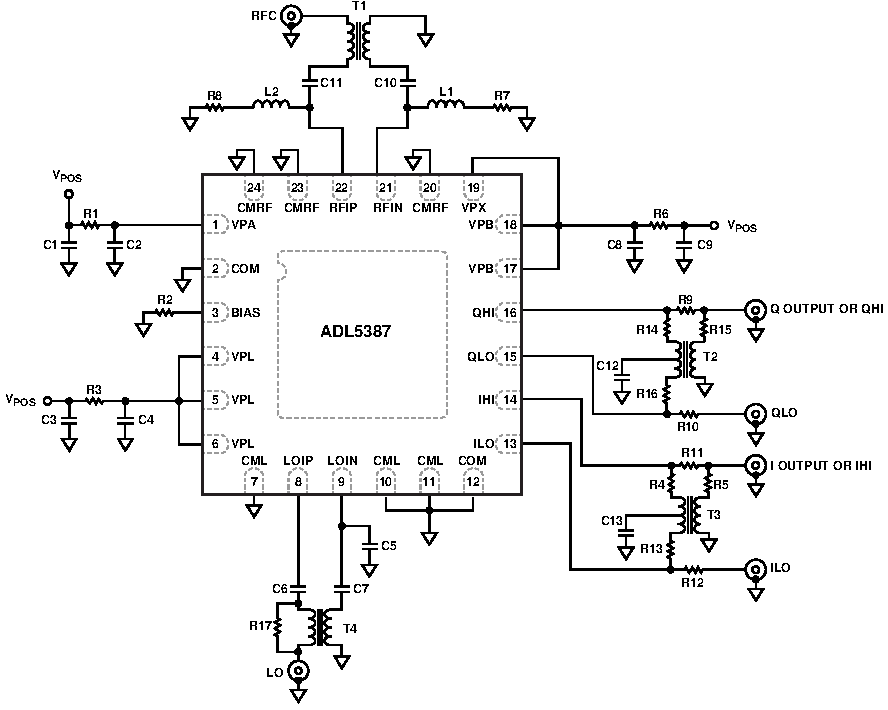
\includegraphics[width=55mm]{../common/ic/ADL5387_page24_schematic.pdf}}
\footnotetext{Diagram extracted from \citeP{ADL5387}.
Extraction notes: {\scriptsize
\verb|pdftk ADL5387.pdf cat 24 output page24.pdf|\\
\verb|pdfcrop --margins "-50 -120 -60 -260" --clip page24.pdf image.pdf|\\
\verb|gswin32c.exe -sDEVICE=pdfwrite -dNOPAUSE -dBATCH -dSAFER -dCompatibilityLevel=1.5 -sOutputFile=ADL5387_page24_schematic.pdf image.pdf| % https://superuser.com/questions/184288/how-to-convert-a-pdf-document-to-an-older-version
}}

%---------------------------------------
\begin{proposition}
\label{prop:Rxynmm}
\label{prop:Rxxnmm}
%---------------------------------------
Let $\rvy(n)$ be a \fncte{random sequence},
    $\rvx(n)$    a \fncte{random sequence} with \fncte{auto-correlation} $\Rxx(n,m)$,
and $\Rxy(n,m)$ the \fncte{cross-correlation} of $\rvx$ and $\rvy$ \xref{def:Rxynm}.
\propbox{
  \brb{\begin{array}{M}
    $\rvx$ and $\rvy$ are
    \\\prope{wide sense stationary}
    \\(\prope{WSS}) \xref{def:wss}
  \end{array}}
  \implies
  \brb{\begin{array}{rcll}
    \Rxx(n,m) &=& \Rxx(m) & \forall n\in\Z\\
    \Rxy(n,m) &=& \Rxy(m) & \forall n\in\Z\\
    \text{\xref{def:Rxynm}} && \text{\xref{def:Rxym}}
  \end{array}}
}
\end{proposition}
\begin{proof}
\begin{align*}
  \Rxy(n,m)
     &\eqd \pE\brs{\rvx[n+m]\rvy^\ast[n]}
     &&    \text{by definition of $\Rxy(n,m)$}
     &&    \text{\xref{def:Rxynm}}
   \\&=    \pE\brs{\rvx[n-n+m]\rvy^\ast[n-n]}
     &&    \text{by \prope{wide sense stationary} hypothesis}
   \\&=    \pE\brs{\rvx[m]\rvy^\ast[0]}
   \\&\eqd \Rxy(m)
     && \text{by definition of $\Rxy(m)$}
     && \text{\xref{def:Rxym}}
   \\
  \Rxx(n,m)
     &=    \brlr{\Rxy(n,m)}_{\rvy=\rvx}
   \\&=    \brlr{\Rxy(m)}_{\rvy=\rvx}
     && \text{by previous result}
   \\&= \Rxx(m)
\end{align*}
\end{proof}


\begin{figure}[ht]\color{figcolor}
\centering%
\setlength{\unitlength}{0.08mm}
\begin{tabular}{*{3}{c@{\hspace{1cm}}}c}
$\Real{\Rxx(m)}$ & $\Imag{\Rxx(m)}$ & $|\Rxx(m)|$ & $\angle\Rxx(m)$
\\
\begin{picture}(340,300)(-150,-150)
  %\graphpaper[10](0,0)(600,200)
  \thicklines%
  \color{figcolor}%
  \put(-150,   0){\line(1,0){300} }
  \put(   0,-150){\line(0,1){300} }
  \put( 160,   0){\makebox(0,0)[l]{$f$} }
  \put(-100,   0){\line( 1,1){100} }
  \put( 100,   0){\line(-1,1){100} }
\end{picture}
&
\begin{picture}(340,300)(-150,-150)
  \thicklines%
  \color{figcolor}%
  \put(-150,   0){\line(1,0){300} }
  \put(   0,-150){\line(0,1){300} }
  \put( 160,   0){\makebox(0,0)[l]{$f$} }
  \qbezier(0,0)( 20, 80)( 100, 100)
  \qbezier(0,0)(-20,-80)(-100,-100)
  \put( 100,   0){\line(0, 1){100} }
  \put(-100,   0){\line(0,-1){100} }
\end{picture}
&
\begin{picture}(340,300)(-150,-150)
  \thicklines%
  \color{figcolor}%
  \put(-150,   0){\line(1,0){300} }
  \put(   0,-150){\line(0,1){300} }
  \put( 160,   0){\makebox(0,0)[l]{$f$} }
  \qbezier(0,100)( 20,20)( 100, 0)
  \qbezier(0,100)(-20,20)(-100, 0)
\end{picture}
&
\begin{picture}(340,300)(-150,-150)
  \thicklines%
  \color{figcolor}%
  \put(-150,   0){\line(1,0){300} }
  \put(   0,-150){\line(0,1){300} }
  \put( 160,   0){\makebox(0,0)[l]{$f$} }
  \put( 100,   0){\line(0, 1){100} }
  \put(-100,   0){\line(0,-1){100} }
  \put(-100,-100){\line(1, 1){200} }
\end{picture}
\\
(\prope{symmetric}) & (\prope{anti-symmetric}) & (\prope{symmetric}) & (\prope{anti-symmetric})
\end{tabular}
\caption{
   \fncte{auto-correlation} $\Rxx(m)$
   \label{fig:Rxxm}
   }
\end{figure}

%---------------------------------------
\begin{corollary}
\label{cor:Rxxm}
\label{cor:Rxym}
%---------------------------------------
Let $\rvx(n)$ be a \fncte{random sequence} with \fncte{auto-correlation} $\Rxx(n,m)$,
    $\rvy(n)$    a \fncte{random sequence} with \fncte{auto-correlation} $\Ryy(n,m)$,
and $\Rxy(n,m)$  the \fncte{cross-correlation} of $\rvx$ and $\rvy$ \xxref{def:Rxynm}{def:Rxym}.
%Let $\opS$ be a \structe{system} with input $\rvx(n)$ and output $\rvy(n)$.
\corbox{
  \brb{\begin{array}{FMD}
      (A).&$\rvx$ is \prope{WSS} & and
    \\(B).&$\rvy$ is \prope{WSS} & %and
   %\\(C).&$\opS$ is \prope{LTI} &
  \end{array}}
  \implies
  \brb{\begin{array}{Frc>{\ds}lDD}
      (1).&      \Rxy(m) &=&       \Ryx^\ast(-m)  &                               & and
    \\(2).&      \Rxx(m) &=&       \Rxx^\ast(-m)  & (\prope{conjugate symmetric}) & and
    \\(3).&\Real \Rxx(m) &=& \Real \Rxx     (-m)  & (\prope{symmetric})           & and
    \\(4).&\Imag \Rxx(m) &=&-\Imag \Rxx     (-m)  & (\prope{anti-symmetric})      & and
    \\(5).&\abs{ \Rxx(m)}&=& \abs{ \Rxx     (-m)} & (\prope{symmetric})           & and
    \\(6).&\angle\Rxx(m) &=&-\angle\Rxx     (-m)  & (\prope{anti-symmetric})      &
  \end{array}}
}
\end{corollary}
\begin{proof}
\begin{align*}
  \Rxy(m)
     &= \Rxy(n,m)
     && \text{by \prefp{prop:Rxynmm}}
     && \text{and hypotheses (A),(B)}
   \\&= \Ryx^\ast(n+m,-m)
     && \text{by \prefp{thm:Rxynm}}
     && \text{and hypothesis (B)}
   \\&= \Ryx^\ast(-m)
     && \text{by \prefp{prop:Rxynmm}}
     && \text{and hypothesis (A)}
   \\
  \Rxx(m)
     &= \Rxx(n,m)
     && \text{by \prefp{prop:Rxynmm}}
     && \text{and hypothesis (A)}
   \\&= \Rxx^\ast(n+m,-m)
     && \text{by \prefp{thm:Rxynm}}
     && \text{and hypothesis (B)}
   \\&= \Rxx^\ast(-m)
     && \text{by \prefp{prop:Rxynmm}}
     && \text{and hypothesis (A)}
  \\
  \Real \Rxx(m)
    &=  \Real\brs{\Rxx^\ast(-m)}
    && \text{by (2)}
  \\&=  \frac{1}{2}\brs{\Rxx^\ast(-m) + \Rxx^{\ast\ast}(-m)}
    && \text{by definition of $\Real$}
    && \text{\xref{def:Re}}
  \\&=  \frac{1}{2}\brs{\Rxx^\ast(-m) + \Rxx(-m)}
    && \text{by \prope{involutory} property of \structe{star-algebra}s}
    && \text{\xref{def:staralg}}
  \\&=  \frac{1}{2}\brs{\Rxx(-m) + \Rxx^\ast(-m)}
  \\&=  \Real\Rxx(-m)
    && \text{by definition of $\Real$}
    && \text{\xref{def:Re}}
  \\
  \Imag \Rxx(m)
    &=  \Imag\brs{\Rxx^\ast(-m)}
    && \text{by (2)}
  \\&=  \frac{1}{2}\brs{\Rxx^\ast(-m) - \Rxx^{\ast\ast}(-m)}
    && \text{by definition of $\Imag$}
    && \text{\xref{def:Im}}
  \\&=  \frac{1}{2}\brs{\Rxx^\ast(-m) - \Rxx(-m)}
    && \text{by \prope{involutory} property of \structe{star-algebra}s.}
    && \text{\xref{def:staralg}}
  \\&=  -\frac{1}{2}\brs{\Rxx(-m) - \Rxx^\ast(-m)}
  \\&=  -\Imag\Rxx(-m)
    && \text{by definition of $\Imag$}
    && \text{\xref{def:Im}}
  \\
  \abs{ \Rxx(m) }
    &\eqd \sqrt{ \brs{\Real\Rxx( m)}^2 + \brs{ \Imag\Rxx( m)}^2 }
  \\&=    \sqrt{ \brs{\Real\Rxx(-m)}^2 + \brs{-\Imag\Rxx(-m)}^2 }
    &&    \text{by (3) and (4)}
  \\&=    \sqrt{ \brs{\Real\Rxx(-m)}^2 + \brs{ \Imag\Rxx(-m)}^2 }
  \\&\eqd \abs{ \Rxx(-m) }
  \\
  \angle{ \Rxx(m) }
    &\eqd \arctan\brs{ \frac{\Imag\Rxx(m)}{\Real\Rxx(m)} }
  \\&=    \arctan\brs{ \frac{-\Imag\Rxx(-m)}{\Real\Rxx(-m)} }
    &&    \text{by (3) and (4)}
  \\&=   -\arctan\brs{ \frac{\Imag\Rxx(-m)}{\Real\Rxx(-m)} }
  \\&\eqd -\angle{ \Rxx(-m) }
\end{align*}
\end{proof}

%=======================================
\section{Spectral density}
%=======================================
%---------------------------------------
\begin{definition}
\label{def:Szxx}
\label{def:Szxy}
%---------------------------------------
Let $\rvx(n)$ and $\rvy(n)$ be \prope{wide sense stationary} \fncte{random sequence}s
with auto-correlation $\Rxx(m)$ and cross-correlation $\Rxy(m)$.
Let $\opZ$ be the \ope{Z-transform operator}\ifsxref{dsp}{def:opZ}.
\\
\defbox{\begin{array}{MMrcl}
   The \opd{z-domain cross spectral density} & (\opd{CSD}) $\ZSxy(z)$ of $\vx$ and $\vy$ is
     \\\mc{5}{l}{\ds\Szxy(z) \eqd \opZ{\Rxy(m)} \eqd \sum_{m\in\Z} \Rxy(m) z^{-m}}
     \\
   The \opd{z-domain power spectral density} & (\opd{PSD}) $\ZSxx(z)$ of $\vx$ is & \Szxx(z) &\eqd& \brlr{\Szxy(z)}_{\rvy(n)=\rvx(n)}
\end{array}}
\end{definition}

%---------------------------------------
\begin{definition}
\label{def:psd}
\label{def:csd}
\label{def:Swxx}
\label{def:Swxy}
%---------------------------------------
Let $\rvx(n)$ and $\rvy(n)$ be \prope{wide sense stationary} \fncte{random sequence}s
with auto-correlation $\Rxx(m)$ and cross-correlation $\Rxy(m)$.
Let $\opDTFT$ be the \ope{Discrete Time Fourier Transform} (\ope{DTFT}) operator\ifsxref{dtft}{def:dtft}.
\\
\defbox{\begin{array}{M rclcl}
  The \opd{auto-spectral density}
  \\$\Swxx(\omega)$ of $\vx$ is           & \Swxx(\omega) &\eqd& \opDTFT{\Rxx(m)} &\eqd& \ds \sum_{m\in\Z} \Rxx(m) e^{-i\omega m}
  \\The \opd{cross spectral density}
  \\(\opd{CSD}) $\Swxy(\omega)$ of $\vx$ and $\vy$ is & \Swxy(\omega) &\eqd& \opDTFT{\Rxy(m)} &\eqd& \ds \sum_{m\in\Z} \Rxy(m) e^{-i\omega m}
  \\\mc{6}{M}{The \opd{auto-spectral density} is also called \opd{power spectral density} (\opd{PSD}).}
\end{array}}
\end{definition}

%---------------------------------------
\begin{theorem}
\label{thm:ZSxy_sym}
%---------------------------------------
Let $\opS$ be a system with \fncte{impulse response} $\fh(n)$,
\fncte{input} $\rvx(n)$, and \fncte{output} $\rvy(n)$.
\thmbox{
  \brb{\begin{array}{MD}
    \mc{2}{M}{$\rvx$ and $\rvy$ are \prope{wide sense stationary}}
  \end{array}}
  \implies
  \brb{\begin{array}{F>{\ds}rc>{\ds}lD}
       (1).&\Szxx(z) &=& \Szxx^\ast\brp{\frac{1}{z^\ast}}             & and
     \\(2).&\Szyx(z) &=& \Szxy^\ast\brp{\frac{1}{z^\ast}}             &
  \end{array}}
  }
\end{theorem}
\begin{proof}
\begin{align*}
  \ZSyx(z)
     &\eqd \opZ \Ryx(m)
    && \text{by definition of $\ZSxy(z)$}                          && \text{\xref{def:csd}}
  \\&\eqd \sum_{m\in\Z}\Ryx(m) z^{-m}
    && \text{by definition of $\opZ$}                              && \text{\xref{def:opZ}}
  \\&\eqd \sum_{m\in\Z} \Rxy^\ast(-m) z^{-m}
    && \text{by \prefp{cor:Rxym}}
  \\&= \brs{\sum_{m\in\Z} \Rxy(-m) (z^\ast)^{-m}}^\ast
    && \text{by \prope{antiautomorphic} property of *-algebras}    && \text{\xref{def:staralg}}
  \\&= \brs{\sum_{-p\in\Z} \Rxy(p) (z^\ast)^{p}}^\ast
    && \text{where $p\eqd -m$}                                     && \text{$\implies$ $m=-p$}
  \\&= \brs{\sum_{p\in\Z} \Rxy(p) (z^\ast)^{p}}^\ast
    && \text{by \prope{absolutely summable} property}              && \text{\xref{def:spllR}}
  \\&= \brs{\sum_{p\in\Z} \Rxy(p) \brp{\frac{1}{z^\ast}}^{-p}}^\ast
  \\&= \ZSxy^\ast\brp{\frac{1}{z^\ast}}
    && \text{by definition of $\opZ$}                              && \text{\xref{def:opZ}}
  \\
  \ZSxx(z)
    &= \brlr{\ZSxy(z)}_{\rvy=\rvx}
  \\&= \brlr{\ZSyx^\ast(z)}_{\rvy=\rvx}
  \\&= \brlr{\ZSxy^\ast\brp{\frac{1}{z^\ast}}}_{\rvy=\rvx}
    && \text{by (2)---previous result}
  \\&= \ZSxx^\ast\brp{\frac{1}{z^\ast}}
\end{align*}
\end{proof}

%---------------------------------------
\begin{corollary}
\label{cor:Swxy_sym}
%---------------------------------------
Let $\opS$ be a system with \fncte{impulse response} $\fh(n)$,
\fncte{input} $\rvx(n)$, and \fncte{output} $\rvy(n)$.
\corbox{
  \brb{\begin{array}{FMD}
    (A).& $\fh$ is \prope{LTI} & and\\
    (B).& \mc{2}{M}{$\rvx$ and $\rvy$ are \prope{WSS}}
  \end{array}}
  \implies
  \brb{\begin{array}{F>{\ds}rc>{\ds}lDD}
       (1).&\Swxy^\ast(\omega) &=& \ds \Swyx(\omega)          & (\prope{conjugate-symmetric}) & and
     \\(2).&\Swxx^\ast(\omega) &=& \ds \Swxx(\omega)          & (\prope{conjugate symmetric}) & and
     \\(3).&\Swxx(\omega)      &\in& \R                       & (\prope{real-valued})         &
  \end{array}}
  }
\end{corollary}
\begin{proof}
\begin{align*}
   \Swxy^\ast(\omega)
     &= \brlr{\ZSxy^\ast(z)}_{z=e^{i\omega}}
     && \text{by definition of \ope{DTFT}}
     && \text{\xref{def:dtft}}
   \\&= \brlr{\ZSyx^{\ast\ast}\brp{\frac{1}{z^\ast}}}_{z=e^{i\omega}}
     && \text{by \prefp{thm:ZSxy_sym}}
   \\&= \brlr{\ZSyx\brp{\frac{1}{z^\ast}}}_{z=e^{i\omega}}
     && \text{by \prope{involutory} property of \structd{$\invo$-algebra}s}
     && \text{\xref{def:staralg}}
   \\&= \ZSyx\brp{\frac{1}{e^{i\omega\ast}}}
   \\&= \ZSyx\brp{e^{i\omega}}
   \\&= \Swyx\brp{\omega}
     && \text{by definition of \ope{DTFT}}
     && \text{\xref{def:dtft}}
   \\
   \Swxx^\ast(\omega)
     &= \brlr{\ZSxx^\ast(z)}_{z=e^{i\omega}}
     && \text{by definition of \ope{DTFT}}
     && \text{\xref{def:dtft}}
   \\&= \brlr{\ZSxx^{\ast\ast}\brp{\frac{1}{z^\ast}}}_{z=e^{i\omega}}
     && \text{by \prefp{thm:ZSxy_sym}}
   \\&= \brlr{\ZSxx\brp{\frac{1}{z^\ast}}}_{z=e^{i\omega}}
     && \text{by \prope{involutory} property of \structd{$\invo$-algebra}s}
     && \text{\xref{def:staralg}}
   \\&= \ZSxx\brp{\frac{1}{e^{i\omega\ast}}}
   \\&= \ZSxx\brp{e^{i\omega}}
   \\&= \Swxx\brp{\omega}
     && \text{by definition of \ope{DTFT}}
     && \text{\xref{def:dtft}}
   \\&\implies\text{$\Swxx(\omega)$ is \prope{real-valued}}
   \\
   \Swxx^\ast(\omega)
     &= \brlr{\Swxy^\ast(\omega)}_{\rvy=\rvx}
   \\&= \brlr{\Swyx(\omega)}_{\rvy=\rvx}
     && \text{by previous result}
   \\&= \Swxx(\omega)
\end{align*}
\end{proof}

%=======================================
\section{Spectral Power}
%=======================================
The term ``\fncte{spectral power}" is a bit of an oxymoron because ``spectral"
deals with leaving the time-domain for the frequency-domain, howbeit
the concept of power is solidly founded on the concept of time in that power = energy per time.

However, the \prope{Plancherel Formula}, or more generally \prope{Parseval's Identity} \xref{prop:parseval_reconstruction},
demonstrates that power in time can also be calculated in frequency.\footnote{\url{https://math.stackexchange.com/questions/3785037/}}
So, it makes some sense to speak of the term ``spectral power".
Moreover, one way to estimate this power is to average the
Fourier Transforms of the product $\abs{\rvx(n)}^2=\rvx(n)\rvx^\ast(n)$\ldots that is, to use an estimate of
the auto-spectral density $\Swxx(\omega)$.
Thus, an alternate name for \fncte{auto-spectral density} is \fnctb{power spectral density} (PSD).

  %============================================================================
% LaTeX File
% Daniel J. Greenhoe
%============================================================================

%======================================
\section{Operations on Sequences}
%\label{app:dsp}
%\label{app:ztrans}
%======================================





%A digital filter is an operator on a sequence 
%For a wide class of digital filters, this operator is linear.
%This operation can often be more clearly 
%understood by the use of a special transform called the {\em Z-transform} (\prefp{def:opZ}).
%The Z-transform represents linear filters by ratios of polynomials
%(a polynomial divided by a polynomial) in a free variable $z$.
%The roots of the numerator polynomial are called \structe{zeros}.
%The roots of the denominator polynomial are called \structe{poles}.
%The location in the $z$-plane of these poles and zeros 
%determine the behavior of the filter operation.




%======================================
%\subsection{Operations}
%======================================
%======================================
\subsection{Convolution operator}
%======================================
\ifdochasnot{seq}{
%--------------------------------------
\begin{definition}
\label{def:sequence}
\label{def:seq}
\footnote{
  \citerp{bromwich1908}{1},
  \citerpgc{thomson2008}{23}{143484367X}{Definition 2.1},
  \citerpg{joshi1997}{31}{8122408265}
  }
\label{def:tuple}
%--------------------------------------
Let $\clFyx$ be the set of all functions from a set $\setY$ to a set $\setX$.
Let $\Z$ be the set of integers.
\defbox{\begin{array}{l}
  \text{A function $\ff$ in $\clFyx$ is a \hid{sequence} over $\setX$ if $\setY=\Z$.}\\
  \text{A sequence may be denoted in the form $\ds\seqxZ{x_n}$ or simply as $\ds\seqn{x_n}$.}\\
  %\text{A function $\ff$ in $\clFyx$ is an \hid{n-tuple} over $\setX$ if $\setY=\setn{1,2,\ldots,\xN}$.}\\
  %\text{An n-tuple may be denoted in the form $\ds\tuplexn{x_n}$ or simply as $\ds\tuplen{x_n}$.}
\end{array}}
\end{definition}
  }

%--------------------------------------
\begin{definition}
\footnote{
  \citerpgc{kubrusly2011}{347}{0817649972}{Example 5.K}
  }
\label{def:spllR}
\label{def:spllF}
%--------------------------------------
Let $\fieldF$ be a \structe{field} \xref{def:field}.
\defboxt{
  The \structd{space of all absolutely square summable sequences} $\spllF$ over $\F$ is defined as
  \\\indentx$\ds\spllF\eqd\set{\seqxZ{x_n}}{\sum_{n\in\Z}\abs{x_n}^2 < \infty}$
  }
\end{definition}

The space $\spllR$ is an example of a \structe{separable Hilbert space}. 
In fact, $\spllR$ is the \emph{only} separable Hilbert space in the sense that all separable Hilbert spaces
are isomorphically equivalent. 
For example, $\spllR$ is isomorphic to $\spLLR$, the \structe{space of all absolutely square Lebesgue integrable functions}.
%That is, their topological structure is the same.
%Differences occur in the nature of operators on the spaces.

%--------------------------------------
\begin{definition}
\label{def:dsp_conv}
\label{def:convd}
\index{convolution}
%--------------------------------------
%Let $\seq{x_n}{n\in\Z}$ and $\seq{y_n}{n\in\Z}$ be sequences \xref{def:seq} in the space $\spllR$ \xref{def:spllR}. 
\defbox{\begin{array}{M}
  The \opd{convolution} operation $\hxs{\convd}$ is defined as 
  \\\indentx
  $\ds{\seqn{x_n}\convd\seqn{y_n}} \eqd \seq{\sum_{m\in\Z} x_{m} y_{n-m}}{n\in\Z}\qquad\scy\forall\seqxZ{x_n},\seqxZ{y_n}\in\spllR$
\end{array}}
\end{definition}

%--------------------------------------
\begin{proposition}
%--------------------------------------
Let $\convd$ be the \structe{convolution operator} \xref{def:dsp_conv}.
\propbox{
  \seqn{x_n}\convd\seqn{y_n} = \seqn{y_n}\convd\seqn{x_n}
  \qquad{\scy\forall\seqxZ{x_n},\seqxZ{y_n}\in\spllR}
  \qquad\text{($\convd$ is \prope{commutative})}
  }
\end{proposition}
\begin{proof}
\begin{align*}
  [x\convd y](n)
    &\eqd \sum_{m\in\Z} x_m y_{n-m}
    &&    \text{by \prefp{def:dsp_conv}}
  \\&=    \sum_{k\in\Z} x_{n-k} y(k)
    &&    \text{where $k=n-m \iff m=n-k$}
  \\&=    \sum_{k\in\Z} x_{n-k} y(k)
    &&    \text{by change commutivity of addition}
  \\&=    \sum_{m\in\Z} x_{n-m} y_m
    &&    \text{by change of variables}
  \\&=    \sum_{m\in\Z} y_m x_{n-m} 
    &&    \text{by \prop{commutative} property of the field over $\C$}
  \\&\eqd \brp{y\convd x}_n
    &&    \text{by \prefp{def:dsp_conv}}
\end{align*}
\end{proof}

%--------------------------------------
\begin{proposition}
\label{prop:conv_knk}
%--------------------------------------
Let $\convd$ be the \structe{convolution operator} \xref{def:dsp_conv}.
\propbox{
  \brb{\begin{array}{F>{\ds}rc>{\ds}lD}
      (A).&\fx[n]\convd\fy[n] &=&   \sum_{k\in\Z} \fx[k]\fy[n-k] & and
    \\(B).&\fx[n],\fy[n]      &\in& \spllR                       &
    \\    &                    \mc{4}{l}{\spllR \quad\text{(\prope{absolutely summable} \xrefnp{def:spllR})}}
  \end{array}}
  \implies
  \brb{\begin{array}{>{\ds}rc>{\ds}l}
     \sum_{k\in\Z} \fx[k]\fy[n+k] &=& \fx[-n]\convd\fy[n]
  \end{array}}
  }
\end{proposition}
\begin{proof}
\begin{align*}
  \sum_{k\in\Z} \fx[k]\fy[n+k] 
    &= \sum_{-p\in\Z} \fx[-p]\fy[n-p] 
    && \text{where $p\eqd -k$}
    && \text{$\implies$ $k=-p$}
  \\&= \sum_{p\in\Z} \fx[-p]\fy[n-p] 
    && \text{by \prope{absolutely summable} hypothesis}
    && \text{\xref{def:spllR}}
  \\&= \sum_{p\in\Z} \fx'[p]\fy[n-p] 
    && \text{where $\fx'[n] \eqd\fx[-n]$}
    && \text{$\implies$ $\fx[-n]=\fx'[n]$}
  \\&\eqd \fx'[n]\convd\fy[n]
    && \text{by definition of \ope{convolution} $\convd$}
    && \text{\xref{def:convd}}
  \\&\eqd \fx[-n]\convd\fy[n]
    && \text{by definition of $\fx'[n]$}
\end{align*}
\end{proof}

%======================================
\subsection{Z-transform}
%======================================
%--------------------------------------
\begin{definition}
\footnote{
  \structe{Laurent series}: \citerpg{aa}{49}{0821821466}
  }
\label{def:opZ}
%--------------------------------------
%Let $\seq{x_n}{n\in\Z}$ be a sequence in the space $\spllR$. %over a ring $\ring$. 
\defbox{\begin{array}{M}
  The \opd{z-transform} $\opZ$ of $\seq{x_n}{n\in\Z}$ is defined as
  \\\indentx
  $\ds\brs{\hxs{\opZ}\seqn{x_n}}(z) \eqd \mcom{\sum_{n\in\Z} x_n z^{-n}}{Laurent series}\qquad\scy\forall\seqn{x_n}\in\spllR$
\end{array}}
\end{definition}


%--------------------------------------
\begin{theorem}
\label{thm:opZ}
%--------------------------------------
Let $X(z)\eqd\opZ\fx[n]$ be the \ope{z-transform} of $\fx[n]$.
\thmbox{
  \brb{\begin{array}{rcl}
    \Zx(z) &\eqd& \opZ\seqn{\fx[n]}
  \end{array}}
  \quad\implies\quad
  \brb{\begin{array}{F>{\ds}lc>{\ds}lCD}
      (1).&\opZ\seqn{\alpha\fx[n]} &=& \alpha\Zx(z)                    & \forall\seqn{x_n}\in\spllR & and
    \\(2).&\opZ\seqn{\fx[n-k]}     &=& z^{-k}\Zx(z)                    & \forall\seqn{x_n}\in\spllR & and
    \\(3).&\opZ\seqn{\fx[-n]}      &=& \Zx\brp{\frac{1}{z}}            & \forall\seqn{x_n}\in\spllR & and
    \\(4).&\opZ\seqn{\fx^\ast[n]}  &=& \Zx^\ast\brp{z^\ast}            & \forall\seqn{x_n}\in\spllR & and
    \\(5).&\opZ\seqn{\fx^\ast[-n]} &=& \Zx^\ast\brp{\frac{1}{z^\ast}}  & \forall\seqn{x_n}\in\spllR &
  \end{array}}
  }
\end{theorem}
\begin{proof}
\begin{align*}
  \alpha\Z\Zx(z)
    &\eqd \alpha \opZ \seqn{\fx[n]}                && \text{by definition of $\Zx(z)$}
  \\&\eqd \alpha \sum_{n\in\Z} \fx[n] z^{-n}       && \text{by definition of $\opZ$ operator}
  \\&\eqd \sum_{n\in\Z} \brp{\alpha\fx[n]} z^{-n}  && \text{by \prope{distributive} property}
  \\&\eqd \opZ\seqn{\alpha\fx[n]}                  && \text{by definition of $\opZ$ operator}
  \\
  z^{-k}\Zx(z) 
    &= z^{-k} \opZ\seqn{\fx[n]}
    && \text{by definition of $\Zx(z)$}
    && \text{(left hypothesis)}
  \\&\eqd z^{-k}\sum_{n=-\infty}^{n=+\infty} \fx[n] z^{-n}
    && \text{by definition of $\opZ$}
    && \text{\xref{def:opZ}}
  \\&=          \sum_{n=-\infty}^{n=+\infty} \fx[n] z^{-n-k}
  \\&=          \sum_{m-k=-\infty}^{m-k=+\infty} \fx[m-k] z^{-m}
    && \text{where $m\eqd n+k$}
    && \text{$\implies$ $n=m-k$}
  \\&=          \sum_{m=-\infty}^{m=+\infty} \fx[m-k] z^{-m}
  \\&=          \sum_{n=-\infty}^{n=+\infty} \fx[n-k] z^{-n}
    && \text{where $n\eqd m$}
  \\&\eqd \opZ\seqn{\fx[n-k]}
    && \text{by definition of $\opZ$}
    && \text{\xref{def:opZ}}
  \\
  \opZ\seqn{\fx^\ast[n]}  
    &\eqd \sum_{n\in\Z}\fx^\ast[n] z^{-n}
    && \text{by definition of $\opZ$}
    && \text{\xref{def:opZ}}
  \\&\eqd \brp{\sum_{n\in\Z}\fx[n] (z^\ast)^{-n}}^\ast
    && \text{by definition of $\opZ$}
    && \text{\xref{def:opZ}}
  \\&\eqd \Zx^\ast(z^\ast)
    && \text{by definition of $\opZ$}
    && \text{\xref{def:opZ}}
  \\
  \opZ\seqn{\fx[-n]}  
    &\eqd \sum_{n\in\Z}\fx[-n] z^{-n}
    && \text{by definition of $\opZ$}
    && \text{\xref{def:opZ}}
  \\&= \sum_{-m\in\Z}\fx[m] z^{m}
    && \text{where $m\eqd -n$}
    && \text{$\implies$ $n=-m$}
  \\&= \sum_{m\in\Z}\fx[m] z^{m}
    && \text{by \prope{absolutely summable} property}
    && \text{\xref{def:spllR}}
  \\&= \sum_{m\in\Z}\fx[m] \brp{\frac{1}{z}}^{-m}
    && \text{by \prope{absolutely summable} property}
    && \text{\xref{def:spllR}}
  \\&\eqd \Zx\brp{\frac{1}{z}}
    && \text{by definition of $\opZ$}
    && \text{\xref{def:opZ}}
  \\
  \opZ\seqn{\fx^\ast[-n]}  
    &\eqd \sum_{n\in\Z}\fx^\ast[-n] z^{-n}
    && \text{by definition of $\opZ$}
    && \text{\xref{def:opZ}}
  \\&= \sum_{-m\in\Z}\fx^\ast[m] z^{m}
    && \text{where $m\eqd -n$}
    && \text{$\implies$ $n=-m$}
  \\&= \sum_{m\in\Z}\fx^\ast[m] z^{m}
    && \text{by \prope{absolutely summable} property}
    && \text{\xref{def:spllR}}
  \\&= \sum_{m\in\Z}\fx^\ast[m] \brp{\frac{1}{z}}^{-m}
    && \text{by \prope{absolutely summable} property}
    && \text{\xref{def:spllR}}
  \\&= \brp{\sum_{m\in\Z}\fx[m] \brp{\frac{1}{z^\ast}}^{-m}}^\ast
    && \text{by \prope{absolutely summable} property}
    && \text{\xref{def:spllR}}
  \\&\eqd \Zx^\ast\brp{\frac{1}{z^\ast}}
    && \text{by definition of $\opZ$}
    && \text{\xref{def:opZ}}
\end{align*}
\end{proof}

%--------------------------------------
\begin{theorem}[\thmd{convolution theorem}]
\label{thm:conv}
%--------------------------------------
Let $\convd$ be the convolution operator \xref{def:dsp_conv}.
%$\seq{x_n}{n\in\Z}$ and $\seq{y_n}{n\in\Z}$ be sequences in the space $\spllR$. %be sequences over a ring $\ring$.
\thmbox{
  \opZ\mcom{\brp{\seqn{x_n}\convd\seqn{y_n}}}{sequence convolution} = \mcom{\brp{\opZ\seqn{x_n}}\;\brp{\opZ\seqn{y_n}}}{series multiplication}
  \qquad{\scy\forall\seqxZ{x_n},\seqxZ{y_n}\in\spllR}
  }
\end{theorem}
\begin{proof}
\begin{align*}
  [\opZ(x\convd y)](z)
    &\eqd \opZ {\left(\sum_{m\in\Z} x_m y_{n-m}\right)}
    &&    \text{by \prefp{def:dsp_conv}}
  \\&\eqd \sum_{n\in\Z} \sum_{m\in\Z} x_m y_{n-m} z^{-n}
    &&    \text{by \prefp{def:opZ}}
  \\&=    \sum_{n\in\Z} \sum_{m\in\Z} x_m y_{n-m} z^{-n}
  \\&=    \sum_{m\in\Z} \sum_{n\in\Z} x_m y_{n-m} z^{-n}
  \\&=    \sum_{m\in\Z} \sum_{k\in\Z} x_m y_k z^{-(m+k)}
    &&    \text{where $k=n-m \iff n=m+k$}
  \\&=    {\left[\sum_{m\in\Z} x_m z^{-m}\right]} 
          {\left[\sum_{k\in\Z} y_k z^{-k}\right]}
  \\&\eqd \brp{\opZ\seqn{x_n}}\;\brp{\opZ\seqn{y_n}}
    &&    \text{by \prefp{def:opZ}}
\end{align*}
\end{proof}



%%---------------------------------------
%\subsection{From z-domain back to time-domain}
%%---------------------------------------
%\begin{figure}
%  \centering
%  \includegraphics[width=\tw/2-2mm]{graphics/iir2n.pdf}
%  \includegraphics[width=\tw/2-2mm]{graphics/dfI_order2_156.pdf}
%  \caption{Direct form 1 order 2 IIR filters\label{fig:df1iir2}}
%\end{figure}
%\begin{align*}
% \Zy(z) &=  b_0X(z) + b_1z^{-1}X(z)  + b_2z^{-2}X(z) - a_1 z^{-1}Y(z) + a_2z^{-2}Y(z)
%  \\\\
%  \fy[n] &= b_0\fx[n] + b_1\fx[n-1] + b_2\fx[n-2] - a_1\fy[n-1] - a_2\fy[n-2]
%\end{align*}
%
%%---------------------------------------
%\begin{example}
%%---------------------------------------
%See \prefpp{fig:df1iir2}
%
%$\ds{\frac{3z^2 + 5z + 7}{2z^2 + 10z + 12}}$
%=
%$\ds{\frac{3z^2 + 5z + 7}{2\brp{z^2 + 5z + 6}}}$
%=
%$\ds{\frac{\brp{\sfrac{3}{2}z^2 + \sfrac{5}{2}z + \sfrac{7}{2}}}
%               {z^2 + 5z + 6}}$
%=
%$\ds{\frac{\brp{\sfrac{3}{2} + \sfrac{5}{2}z^{-1} + \sfrac{7}{2}z^{-2}}}
%               {1 + 5z^{-1} + 6z^{-2}}}$
%\end{example}
%
%
%%=======================================
%\subsection{Zero locations}
%%=======================================
%The system property of \prope{minimum phase} is defined in \pref{def:minphase} (next) and 
%illustrated in \prefpp{fig:pz_minphase}.
%\begin{figure}[h]
%  \centering%
%  \begin{tabular}{cc}
%    \includegraphics{graphics/pz_realcoefs.pdf}%
%    &\includegraphics{graphics/pz_minphase.pdf}%
%    \\\emph{not} minimum phase & \prope{minimum phase}
%  \end{tabular}
%  \caption{Minimum Phase filter\label{fig:pz_minphase}}
%\end{figure}
%%--------------------------------------
%\begin{definition}
%\footnote{
%  \citerpg{farina2000}{91}{0471384569},
%  \citerpg{dumitrescu2007}{36}{1402051247}
%  }
%\label{def:minphase}
%\index{minimum phase}
%%--------------------------------------
%Let $\Zx(z)\eqd\opZ\seqn{x_n}$ be the \fncte{z transform} \xref{def:opZ} of a sequence $\seqxZ{x_n}$ in $\spllR$.
%Let $\seqxZ{z_n}$ be the \structe{zeros} of $\Zx(z)$.
%\defbox{\begin{array}{M}
%  The sequence $\seqn{x_n}$ is \hid{minimum phase} if
%  \\\indentx$\ds\mcom{\abs{z_n}<1\qquad \forall n\in\Z}{$\Zx(z)$ has all its \structe{zeros} inside the unit circle}$
%\end{array}}
%\end{definition}
%
%The impulse response of a minimum phase filter has most of its energy concentrated
%near the beginning of its support, as demonstrated next.
%%--------------------------------------
%\begin{theorem}[\thmd{Robinson's Energy Delay Theorem}]
%\footnote{
%  \citerpg{dumitrescu2007}{36}{1402051247},
%  \citor{robinson1962},  % referenced by claerbout1976
%  \citorc{robinson1966}{???},  % referenced by online thesis
%  \citerpp{claerbout1976}{52}{53}
%  %\citerp{os}{291}\\
%  %\citerp{mallat}{253}
%  }
%\label{thm:ztr_redp}
%\label{thm:redt}
%\index{minimum phase!energy}
%\index{energy}
%%--------------------------------------
%Let $\fp(z)\eqd\sum_{n=0}^\xN a_n z^{-n}$ 
%and $\fq(z)\eqd\sum_{n=0}^\xN b_n z^{-n}$ 
%be polynomials.
%\thmbox{
%  \brb{\begin{array}{lMD}
%    \fp & is \prope{minimum phase} & and\\
%    \fq & is \emph{not} minimum phase & 
%  \end{array}}
%  \implies
%  \mcom{\sum_{n=0}^{m-1} \abs{a_n}^2}{\parbox{20mm}{``energy" of the first $m$ coefficients of $\fp(z)$}} \ge 
%  \mcom{\sum_{n=0}^{m-1} \abs{b_n}^2}{\parbox{20mm}{``energy" of the first $m$ coefficients of $\fq(z)$}} 
%  \qquad \forall 0\le m\le\xN
%  }
%\end{theorem}
%
%But for more \prope{symmetry}, put some zeros inside and some outside the unit circle.
%
%\begin{figure}[h]
%\begin{center}
%\footnotesize
%\setlength{\unitlength}{0.08mm}
%\begin{tabular}{|c|c|}
%  \hline
%  Daubechies-4 & Symlets-4
%  \\\hline
%  \includegraphics{graphics/D4_pz.pdf}&\includegraphics{graphics/S4_pz.pdf} \\
%  \includegraphics{graphics/d4_phi_h.pdf}&\includegraphics{graphics/s4_phi_h.pdf}\\ 
%  \hline
%  \prope{minimum phase} & \emph{not} minimum phase
%  \\\hline
%\end{tabular}
%\caption{
%   Daubechies-4 and Symlet-4 scaling functions pole-zero plots
%   \label{fig:pz_d4}
%   }
%\end{center}
%\end{figure}
%%--------------------------------------
%\begin{example}
%%--------------------------------------
%An example of a minimum phase polynomial is the Daubechies-4 scaling function.
%%This function is generated by a minimum phase filter.
%The minimum phase polynomial causes most of the energy to be concentrated near the origin, making it very \hie{asymmetric}.
%In contrast, the Symlet-4 has a design very similar to that of Daubechies-4, 
%but the selected zeros are not all within the unit circle in the complex $z$ plane.
%This results in a scaling function that is more symmetric and less contrated near the origin.
%Both scaling functions are illustrated in \prefpp{fig:pz_d4}.
%\end{example}
%
%%=======================================
%\subsection{Pole locations}
%%=======================================
%%---------------------------------------
%%\subsection{Stability and pole location}
%%---------------------------------------
%For a stable filter, put all the poles \emph{inside} the unit circle.
%%--------------------------------------
%\begin{theorem}
%\index{stability}
%%--------------------------------------
%A causal LTI filter is {\bf stable} if all of its poles are {\bf inside} the unit circle.
%\end{theorem}
%
%\begin{figure}[ht]
%  \centering%
%  \begin{tabular}{c@{\hspace{1cm}}c}
%     \includegraphics{graphics/pz_stable.pdf}
%    &\includegraphics{graphics/pz_unstable.pdf}
%    \\stable & unstable
%\end{tabular}
%  \caption{
%     Pole-zero plot stable/unstable causal LTI filters \xref{ex:pz_unstable}
%     \label{fig:pz_unstable}
%     }
%\end{figure}
%%--------------------------------------
%\begin{example}
%\label{ex:pz_unstable}
%%--------------------------------------
%Stable/unstable filters are illustrated in \prefpp{fig:pz_unstable}.
%\end{example}
%
%
%%---------------------------------------
%%\subsection{The Reappearing Roots: Now you don't see them, now you do}
%%---------------------------------------
%
%True or False? This filter has no poles:
%
%  $\ds H(z)= b_0 + b_1 z^{-1} + b_2 z^{-2}$
%
%\includegraphics{graphics/dfI_order2_fir.pdf}
%
%
%\begin{align*}
%  H(z)
%    &= b_0 + b_1 z^{-1} + b_2 z^{-2}
%     = \frac{z^2}{z^2} \times \frac{b_0 + b_1 z^{-1} + b_2 z^{-2}}{1}
%     = \frac{b_0 z^2 + b_1 z^{1} + b_2 }{z^2}
%\end{align*}
%
%\includegraphics{graphics/pz_pole00.pdf}
%
%%---------------------------------------
%\subsection{Mirroring for real coefficients}
%%---------------------------------------
%\begin{figure}
%  \centering
%  \includegraphics{graphics/pz_minphase.pdf}%
%  \includegraphics{graphics/pz_realcoefs_11.pdf}
%\caption{Conjugate pair structure yielding real coefficients\label{fig:realcoefs}}
%\end{figure}
%
%If you want real coefficients, choose poles and zeros in conjugate pairs (next).
%%---------------------------------------
%\begin{proposition}
%%---------------------------------------
%\propbox{
%  \brb{\begin{array}{M}
%    \structe{zeros} and \structe{poles}\\
%    occur in \structe{conjugate pairs} 
%  \end{array}}
%  \quad\implies\quad
%  \brb{\begin{array}{M}
%    \structe{coefficients} \\
%    are \prope{real}.
%  \end{array}}
%  }
%\end{proposition}
%\begin{proof}
%\begin{align*}
%  \brp{z-p_1}\brp{z-p_1^*}
%    &= \brs{z-\brp{a+ib}} \brs{z-\brp{a-ib}}
%  \\&= z^2 +\brs{-a+ib-ib-a}z - \brs{ib}^2
%  \\&= z^2 -2a z + b^2
%\end{align*}
%\end{proof}
%
%%---------------------------------------
%\begin{example}
%%---------------------------------------
%See \prefpp{fig:realcoefs}.
%\begin{align*}
%  H(z)   &= G\frac{\brs{z-z_1}\brs{z-z_2}}
%                  {\brs{z-p_1}\brs{z-p_2}}
%          = G\frac{\brs{z-\brp{1+i}}\brs{z-\brp{1-i}}}
%                  {\brs{z-\brp{-\sfrac{2}{3}+i\sfrac{1}{2}}}\brs{z-\brp{-\sfrac{2}{3}-i\sfrac{1}{2}}}}
%       \\&= G\frac{z^2 - z\brs{\brp{1-i}+\brp{1+i}} + \brp{1-i}\brp{1+i}}
%                  {z^2 - z\brs{\brp{-\sfrac{2}{3}+i\sfrac{1}{2}}+\brp{-\sfrac{2}{3}+i\sfrac{1}{2}}} + \brp{-\sfrac{2}{3}+i\sfrac{1}{2}}\brp{-\sfrac{2}{3}+i\sfrac{1}{2}}}
%       \\&= G\frac{z^2 - 2z + 2}
%                  {z^2 - \sfrac{4}{3}z + \brp{\sfrac{4}{3}+\sfrac{1}{4}}}
%          = G\frac{z^2 - 2z + 2}
%                  {z^2 - \sfrac{4}{3}z + \sfrac{19}{12}}
%\end{align*}
%\end{example}
%
%
%%=======================================
%\subsection{Rational polynomial operators}
%%=======================================
%A digital filter is simply an operator on $\spllR$.
%If the digital filter is a causal LTI system, then it can be expressed as 
%a rational polynomial in $z$ as shown next.
%
%%=======================================
%\begin{lemma}
%%=======================================
%A causal LTI operator $\mathcal{H}$ can be expressed as a rational expression $\Zh(z)$.
%\begin{align*}
% \Zh(z) &= \frac{b_0 + b_1z^{-1} + b_2z^{-2} + \cdots + b_Nz^{-N}}
%                {1   + a_1z^{-1} + a_2z^{-2} + \cdots + a_Nz^{-N}}
%   \\   &= \frac{\sum\limits_{n=0}^{N} b_n z^{-n}}
%                {1   + \sum\limits_{n=1}^{N} a_n z^{-n}}
%\end{align*}
%\end{lemma}
%
%
%A filter operation $\Zh(z)$ can be expressed as a product of its roots (poles and zeros).
%\begin{align*}
% \Zh(z) &= \frac{b_0 + b_1z^{-1} + b_2z^{-2} + \cdots + b_\xN z^{-\xN}}
%                {1   + a_1z^{-1} + a_2z^{-2} + \cdots + a_\xN z^{-\xN}}
%   \\   &= \alpha\frac{(z-z_1)(z-z_2)\cdots(z-z_\xN)}
%                {(z-p_1)(z-p_2)\cdots(z-p_\xN)}
%\end{align*}
%where $\alpha$ is a constant, $z_i$ are the zeros, and $p_i$ are the poles.
%The poles and zeros of such a rational expression are often plotted in the z-plane with a unit circle
%about the origin (representing $z=e^{i\omega}$).
%Poles are marked with $\times$ and zeros with $\bigcirc$.
%An example is shown in \prefp{fig:pz}.  
%Notice that in this figure the zeros and poles are either real or occur in 
%complex conjugate pairs.
%
%\begin{figure}[ht]
%  \centering
%  \includegraphics{graphics/pz_realcoefs.pdf}
%  \caption{
%     Pole-zero plot for rational expression with real coefficients
%     \label{fig:pz}
%     }
%\end{figure}
%
%
%
%%======================================
%\subsection{Filter Banks}
%%======================================
%\structe{Conjugate quadrature filters} (next definition) are used in \structe{filter banks}.
%If $\Zx(z)$ is a \structe{low-pass filter}, then the conjugate quadrature filter of $\Zy(z)$ is a \structe{high-pass filter}.
%
%%--------------------------------------
%\begin{definition}
%\footnote{
%  \citerpg{strang1996}{109}{0961408871},
%  \citerppgc{haddad1992}{256}{259}{0323138365}{section 4.5},
%  \citerpgc{vaidyanathan1993}{342}{0136057187}{(7.2.7), (7.2.8)},
%  \citor{smith1984},
%  \citor{smith1986},
%  \citor{mintzer1985}
%  }
%\label{def:cqf}
%%--------------------------------------
%Let $\seqxZ{x_n}$ and $\seqxZ{y_n}$ be \structe{sequences} \xref{def:seq} in $\spllR$ \xref{def:spllR}.
%\defboxt{
%  The sequence $\seqn{y_n}$ is a \fnctd{conjugate quadrature filter} with shift $\xN$ with respect to $\seqn{x_n}$ if
%  \\\indentx$\ds y_n = \pm(-1)^n x^\ast_{\xN-n}$\\
%  A \structe{conjugate quadrature filter} is also called a \hid{CQF} or a \hid{Smith-Barnwell filter}.
%  \\
%  Any triple $\otriple{\seqn{x_n}}{\seqn{y_n}}{\xN}$ in this form is said to satisfy the
%  \\\indentx\propd{conjugate quadrature filter condition} or
%  the \propd{CQF condition}.
%  }
%\end{definition}
%
%%--------------------------------------
%\begin{theorem}[\thmd{CQF theorem}]
%%\begin{theorem} % [\thmd{conjugate quadrature filters}/\thmd{CQF}/\thmd{Smith-Barnwell filters}]
%\label{thm:cqf}
%\footnote{
%  %\citerpgc{dau}{135}{0898712742}{(5.1.34)},
%  %\citerpgc{vidakovic}{59}{0471293652}{(3.34)},
%  \citerpg{strang1996}{109}{0961408871},
%  \citerppgc{mallat}{236}{238}{012466606X}{(7.58),(7.73)},
%  \citerppgc{haddad1992}{256}{259}{0323138365}{section 4.5},
%  \citerpgc{vaidyanathan1993}{342}{0136057187}{(7.2.7), (7.2.8)}
%  }
%%--------------------------------------
%Let $\Dy(\omega)$ and $\Dx(\omega)$ be the \ope{DTFT}s \xref{def:dtft} of the sequences $\seqxZ{y_n}$ and $\seqxZ{x_n}$, respectively, in $\spllR$ \xref{def:spllR}.
%\thmboxt{
%  $\ds\begin{array}{>{\ds}r c rc>{\ds}l DD}
%    \mcom{y_{n} = \pm (-1)^n x^\ast_{\xN-n}}
%         {(1) \structe{CQF} in ``time"}
%      &\iff& \Zy(z)      &=& \pm (-1)^\xN z^{-\xN} \Zx^\ast\brp{\frac{-1}{z^\ast}}   & (2)& \structe{CQF} in ``z-domain"
%    \\&\iff& \Dy(\omega) &=& \pm (-1)^\xN e^{-i\omega\xN} \Dx^\ast(\omega+\pi)       & (3)& \structe{CQF} in ``frequency"
%    \\&\iff& x_{n}       &=& \pm (-1)^\xN (-1)^n y^\ast_{\xN-n}                      & (4)& ``reversed" \structe{CQF} in ``time"
%    \\&\iff& \Zx(z)      &=& \pm z^{-\xN} \Zy^\ast\brp{\frac{-1}{z^\ast}}            & (5)& ``reversed" \structe{CQF} in ``z-domain"
%    \\&\iff& \Dx(\omega) &=& \pm e^{-i\omega\xN} \Dy^\ast(\omega+\pi)                & (6)& ``reversed" \structe{CQF} in ``frequency"
%  \end{array}$
%  \\$\indentx\scy\forall\xN\in\Z$
%  }
%\end{theorem}
%\begin{proof}
%\begin{enumerate}
%  \item Proof that $(1)\implies(2)$:
%    \begin{align*}
%      \Zy(z)
%        &= \sum_{n\in\Z}  y_{n}  z^{-n}
%        && \text{by definition of \fncte{z-transform}}
%        && \text{\xref{def:opZ}}
%      \\&= \sum_{n\in\Z} \mcom{(\pm) (-1)^n x^\ast_{\xN-n}}{\structe{CQF}} z^{-n}
%        && \text{by (1)}
%      \\&= \pm\sum_{m\in\Z} (-1)^{\xN-m} x_m^\ast z^{-(\xN-m)}
%        && \text{where $m\eqd\xN-n \implies$}
%        && \text{$n=\xN-m$}
%      \\&= \pm (-1)^\xN z^{-\xN}
%           \sum_{m\in\Z}(-1)^{-m} x_m^\ast \brp{z^{-1}}^{-m}
%      \\&= \pm (-1)^\xN z^{-\xN}
%           \sum_{m\in\Z} x^\ast_m \brp{-\frac{1}{z}}^{-m}
%      \\&= \pm (-1)^\xN z^{-\xN}
%           \brs{\sum_{m\in\Z} x_m \brp{-\frac{1}{z^\ast}}^{-m}}^\ast
%      \\&= \pm (-1)^\xN z^{-\xN}\Zx^\ast\brp{\frac{-1}{z^\ast}}
%        && \text{by definition of \fncte{z-transform}}
%        && \text{\xref{def:opZ}}
%    \end{align*}
%
%  \item Proof that $(1)\impliedby(2)$:
%    \begin{align*}
%      \Zy(z)
%        &= \pm (-1)^\xN z^{-\xN} \Zx^\ast\brp{\frac{-1}{z^\ast}}
%        && \text{by (2)}
%      \\&= \pm (-1)^\xN z^{-\xN} \brs{\sum_{m\in\Z} x_m \brp{\frac{-1}{z^\ast}}^{-m}}^\ast
%        && \text{by definition of \fncte{z-transform}}
%        && \text{\xref{def:opZ}}
%      \\&= \pm (-1)^\xN z^{-\xN} \brs{\sum_{m\in\Z} x^\ast_m \brp{-z^{-1}}^{-m}}
%        && \text{by definition of \fncte{z-transform}}
%        && \text{\xref{def:opZ}}
%      \\&= \sum_{m\in\Z}(\pm) (-1)^{\xN-m} x^\ast_m z^{-(\xN-m)}
%      \\&= \sum_{m\in\Z}(\pm) (-1)^{n} x^\ast_{\xN-n} z^{-n}
%        && \text{where $n=\xN-m$ $\implies$}
%        && \text{$m\eqd\xN-n$}
%      \\&\implies x_n = \pm (-1)^n x^\ast_{\xN-n}
%    \end{align*}
%
%  \item Proof that $(1)\implies(3)$:
%    \begin{align*}
%      \Dy(\omega)
%        &\eqd \Zx(z)\Big|_{z=e^{i\omega}}
%        &&    \text{by definition of \fncte{DTFT} \xref{def:dtft}}
%      \\&=    \brs{\pm (-1)^\xN z^{-\xN}\Zx\brp{\frac{-1}{z^\ast}}}_{z=e^{i\omega}}
%        &&    \text{by (2)}
%      \\&=    \pm (-1)^\xN e^{-i\omega\xN}\Zx\brp{e^{i\pi}e^{\i\omega}}
%      \\&=    \pm (-1)^\xN e^{-i\omega\xN}\Zx\brp{e^{i(\omega+\pi)}}
%      \\&=    \pm (-1)^\xN e^{-i\omega\xN}\Dx\brp{\omega+\pi}
%        &&    \text{by definition of \fncte{DTFT} \xref{def:dtft}}
%    \end{align*}
%
%  \item Proof that $(1)\implies(6)$:
%    \begin{align*}
%      \Dx(\omega) 
%        &= \sum_{n\in\Z}  y_{n}  e^{-i\omega n}
%        && \text{by definition of \fncte{DTFT}}
%        && \text{\xref{def:dtft}}
%      \\&= \sum_{n\in\Z} \mcom{\pm (-1)^n x_{\xN-n}^\ast}{\structe{CQF}} e^{-i\omega n}
%        && \text{by (1)}
%      \\&= \sum_{m\in\Z}\pm (-1)^{\xN-m} x_m^\ast e^{-i\omega (\xN-m)}
%        && \text{where $m\eqd\xN-n \implies$}
%        && \text{$n=\xN-m$}
%      \\&= \pm (-1)^\xN e^{-i\omega\xN}
%           \sum_{m\in\Z}(-1)^m x_m^\ast e^{i\omega m}
%      \\&= \pm (-1)^\xN e^{-i\omega\xN}
%           \sum_{m\in\Z}e^{i\pi m} x_m^\ast e^{i\omega m}
%      \\&= \pm (-1)^\xN e^{-i\omega\xN}
%           \sum_{m\in\Z}x_m^\ast e^{i (\omega+\pi )m}
%      \\&= \pm (-1)^\xN e^{-i\omega\xN}
%           \left[ \sum_{m\in\Z}x_m e^{-i(\omega+\pi )m} \right]^\ast
%      \\&= \pm (-1)^\xN e^{-i\omega\xN}\Dx^\ast\left(\omega+\pi \right)
%        && \text{by definition of \fncte{DTFT}}
%        && \text{\xref{def:dtft}}
%    \end{align*}
%
%  \item Proof that $(1)\impliedby(3)$:
%    \begin{align*}
%      y_n
%        &= \frac{1}{2\pi}\int_{-\pi}^{+\pi} \Dy(\omega) e^{i\omega n} \dw
%        && \text{by \thme{inverse DTFT}}
%        && \text{\xref{thm:idtft}}
%      \\&= \frac{1}{2\pi}\int_{-\pi}^{+\pi} \mcom{\pm (-1)^\xN e^{-i\xN\omega} \Dx^\ast(\omega+\pi)}{right hypothesis} e^{i\omega n} \dw
%        && \text{by right hypothesis}
%      \\&= \pm (-1)^\xN\frac{1}{2\pi}\int_{-\pi}^{+\pi}  \Dx^\ast(\omega+\pi) e^{i\omega(n-\xN)} \dw
%        && \text{by right hypothesis}
%      \\&= \pm (-1)^\xN\frac{1}{2\pi}\int_{0}^{2\pi}  \Dx^\ast(v) e^{i(v-\pi)(n-\xN)} \dv
%        && \text{where $v\eqd\omega+\pi$ $\implies$}
%        && \text{$\omega=v-\pi$}
%      \\&= \pm (-1)^\xN e^{-i\pi(n-\xN)} \frac{1}{2\pi}\int_{0}^{2\pi}  \Dx^\ast(v) e^{iv(n-\xN)} \dv
%      \\&= \pm (-1)^\xN \mcom{(-1)^\xN}{$e^{i\pi N}$} \mcom{(-1)^n}{$e^{-i\pi n}$} 
%           \brs{\frac{1}{2\pi}\int_{0}^{2\pi}  \Dx(v) e^{iv(\xN-n)} \dv}^\ast
%      \\&= \pm (-1)^n x_{\xN-n}^\ast
%        && \text{by \thme{inverse DTFT}}
%        && \text{\xref{thm:idtft}}
%    \end{align*}
%
%  \item Proof that (1)$\iff$(4): % 2013jun14fri
%    \begin{align*}
%      y_{n} = \pm (-1)^n x^\ast_{\xN-n}
%        &\iff (\pm)(-1)^n y_{n} = (\pm)(\pm) (-1)^n (-1)^n x^\ast_{\xN-n}
%      \\&\iff \pm(-1)^n y_{n} = x^\ast_{\xN-n}
%      \\&\iff \brp{\pm(-1)^n y_{n}}^\ast = \brp{x^\ast_{\xN-n}}^\ast
%      \\&\iff \pm(-1)^n y^\ast_{n} = x_{\xN-n}
%      \\&\iff x_{\xN-n} = \pm(-1)^n y^\ast_{n}
%      \\&\iff x_m = \pm(-1)^{\xN-m} y^\ast_{\xN-m}
%        && \text{where $m\eqd \xN-n\implies$}
%        && \text{$n=\xN-m$}
%      \\&\iff x_m = \pm(-1)^{\xN-m} y^\ast_{\xN-m}
%      \\&\iff x_m = \pm(-1)^\xN (-1)^m y^\ast_{\xN-m}
%      \\&\iff x_n = \pm(-1)^\xN (-1)^n y^\ast_{\xN-n}
%        &&    \text{by change of free variables}
%    \end{align*} 
%
%  \item Proofs for (5) and (6): not included. See proofs for (2) and (3).
%\end{enumerate}
%\end{proof}
%
%
%%--------------------------------------
%\begin{theorem}
%\footnote{
%  \citerpp{vidakovic}{82}{83},
%  \citerpp{mallat}{241}{242}
%  }
%\label{thm:cqf_ddw}
%%--------------------------------------
%Let $\Dy(\omega)$ and $\Dx(\omega)$ be the \ope{DTFT}s \xref{def:dtft} of the sequences $\seqxZ{y_n}$ and $\seqxZ{x_n}$, respectively, in $\spllR$ \xref{def:spllR}.
%\thmboxt{
%  Let $y_n = \pm(-1)^n x^\ast_{N-n}$ (\prope{CQF condition}, {\scs\prefp{def:cqf}}). Then\\
%  $\brb{\begin{array}{D@{\qquad}>{\ds}rc>{\ds}lcl@{\qquad}D}
%       (A)&\left.\opddwn  \Dy(\omega)\right|_{\omega=0} = 0
%          &\iff  & \left.\opddwn  \Dx(\omega)\right|_{\omega=\pi}   &=& 0 & (B)
%       \\&&\iff  & \sum_{k\in\Z} (-1)^k k^n  x_k                    &=& 0 & (C)
%       \\&&\iff  & \sum_{k\in\Z} k^n  y_k                           &=& 0 & (D)
%  \end{array}}
%  \quad\scy\forall n\in\Znn$
%  }
%\end{theorem}
%\begin{proof}
%\begin{enumerate}
%  \item Proof that (A)$\implies$(B): 
%    \begin{align*}
%      0
%        &= \opddwn\Dy(\omega)\Big|_{\omega=0}
%        && \text{by (A)}
%      \\&= \opddwn(\pm)(-1)^\xN e^{-i\omega\xN}\Dx^\ast(\omega+\pi)\Big|_{\omega=0}
%        && \text{by \thme{CQF theorem}}
%        && \text{\xref{thm:cqf}}
%      \\&= \brlr{(\pm)(-1)^\xN \sum_{\ell=0}^n \bcoef{n}{\ell} \brs{\opddw}^\ell\brs{e^{-i\omega\xN}}\cdot\brs{\opddw}^{n-\ell}\brs{\Dx^\ast(\omega+\pi)}}_{\omega=0}
%        && \text{by \thme{Leibnitz GPR}}
%        && \text{\xref{lem:LGPR}}
%      \\&= \brlr{(\pm)(-1)^\xN 
%                 \sum_{\ell=0}^n \bcoef{n}{\ell} {-i\xN}^\ell e^{-i\omega\xN}\brs{\opddw}^{n-\ell}\brs{\Dx^\ast(\omega+\pi)}
%                }_{\omega=0}
%      \\&= \brlr{(\pm)(-1)^\xN  \cancelto{1}{e^{-i0\xN}} \sum_{\ell=0}^n \bcoef{n}{\ell} {-i\xN}^\ell \brs{\opddw}^{n-\ell}\brs{\Dx^\ast(\omega+\pi)}}_{\omega=0}
%    \end{align*}
%  \[\begin{array}{r rcl l}
%    \implies & \Dx^{(0)}(\pi) &=& 0 \\
%    \implies & \Dx^{(1)}(\pi) &=& 0 \\
%    \implies & \Dx^{(2)}(\pi) &=& 0 \\
%    \implies & \Dx^{(3)}(\pi) &=& 0 \\
%    \implies & \Dx^{(4)}(\pi) &=& 0 \\
%    \vdots   & \mc{1}{c}{\vdots}    \\
%    \implies & \Dx^{(n)}(\pi) &=& 0 & \text{for $n=0,1,2,\ldots$}
%  \end{array}\]
%
%  \item Proof that (A)$\impliedby$(B): 
%    \begin{align*}
%      0
%        &= \opddwn\Dx(\omega)\Big|_{\omega=\pi}
%        && \text{by (B)}
%      \\&= \opddwn(\pm) e^{-i\omega\xN} \Dy^\ast(\omega+\pi)\Big|_{\omega=\pi}
%        && \text{by \thme{CQF theorem}}
%        && \text{\xref{thm:cqf}}
%      \\&= \brlr{(\pm) \sum_{\ell=0}^n \bcoef{n}{\ell} \brs{\opddw}^\ell\brs{e^{-i\omega\xN}}\cdot\brs{\opddw}^{n-\ell}\brs{\Dy^\ast(\omega+\pi)}}_{\omega=\pi}
%        && \text{by \thme{Leibnitz GPR}}
%        && \text{\xref{lem:LGPR}}
%      \\&= \brlr{(\pm) \sum_{\ell=0}^n \bcoef{n}{\ell} (-i\xN)^\ell e^{-i\omega\xN}\brs{\opddw}^{n-\ell}\brs{\Dy^\ast(\omega+\pi)}}_{\omega=\pi}
%      \\&= \brlr{(\pm) \cancelto{1}{e^{-i\pi\xN}} \sum_{\ell=0}^n \bcoef{n}{\ell} {-i\xN}^\ell \brs{\opddw}^{n-\ell}\brs{\Dy^\ast(\omega+\pi)}}_{\omega=\pi}
%      \\&= \brlr{(\pm) (-1)^\xN \sum_{\ell=0}^n \bcoef{n}{\ell} {-i\xN}^\ell \brs{\opddw}^{n-\ell}\brs{\Dy^\ast(\omega+\pi)}}_{\omega=\pi}
%    \end{align*}
%  \[\begin{array}{r rcl l}
%    \implies & \Dy^{(0)}(0) &=& 0 \\
%    \implies & \Dy^{(1)}(0) &=& 0 \\
%    \implies & \Dy^{(2)}(0) &=& 0 \\
%    \implies & \Dy^{(3)}(0) &=& 0 \\
%    \implies & \Dy^{(4)}(0) &=& 0 \\
%    \vdots   & \mc{1}{c}{\vdots}    \\
%    \implies & \Dy^{(n)}(0) &=& 0 \\
%    \implies & \Dy^{(n)}(0) &=& 0 & \text{for $n=0,1,2,\ldots$}
%  \end{array}\]
%
%
%  \item Proof that (B)$\iff$(C): by \prefp{thm:dtft_ddw}
%  \item Proof that (A)$\iff$(D): by \prefp{thm:dtft_ddw}
%  \item Proof that (CQF)$\notimpliedby$(A): Here is a counterexample: $\Dy(\omega)=0$.
%
%\end{enumerate}
%\end{proof}
%
%
%%---------------------------------------
%\subsection{Inverting non-minimum phase filters}
%%---------------------------------------
%\prope{Minimum phase} filters are easy to invert: each \structe{zero} becomes a \structe{pole} 
%and each \structe{pole} becomes a \structe{zero}.
%\begin{figure}
%\centering
%$\begin{array}{ccccc}
%     \tbox{\includegraphics{graphics/pz_minphase.pdf}}
%    &\tbox{$\times$}
%    &\tbox{\includegraphics{graphics/pz_minphase_inv.pdf}}
%    &\tbox{$=$}
%    &\tbox{$1$}
%  \\
%     \ds\frac{\brp{z-z_1}\brp{z-z_2}\brp{z-z_3}\brp{z-z_4}}
%             {\brp{z-p_1}\brp{z-p_2}\brp{z-p_3}\brp{z-p_4}}
%    &\times
%    &\ds\frac{\brp{z-p_1}\brp{z-p_2}\brp{z-p_3}\brp{z-p_4}}
%             {\brp{z-z_1}\brp{z-z_2}\brp{z-z_3}\brp{z-z_4}}
%    &=
%    &1
%\end{array}$
%\end{figure}
%
%\begin{tabular}{ccccc}
%     \tbox{\includegraphics{graphics/pz_unstable2.pdf}}
%    &\tbox{$\times$}&
%     \tbox{\includegraphics{graphics/pz_allpass.pdf}}
%    &\tbox{$=$}&
%     \tbox{\includegraphics{graphics/pz_unall.pdf}}
%  \\unstable&&all-pass&&stable!
%\end{tabular}
%
%\begin{align*}
%  \abs{A\brp{z}}_{z=e^{i\omega}}
%    &= \frac{1}{r}\abs{\frac{z-r          e^{i\phi}}
%                            {z-\frac{1}{r}e^{i\phi}}}_{z=e^{i\omega}}
%   &&= \abs{\frac{ z- re^{i\phi}}
%                 {rz-  e^{i\phi}}}_{z=e^{i\omega}}
%  \\&= \abs{e^{i\phi}\brp{
%            \frac{e^{-i\phi}z-r}
%                 {rz- e^{i\phi}}}}_{z=e^{i\omega}}
%   &&= \abs{z\brp{
%            \frac{e^{-i\phi}-rz^{-1}}
%                 {rz- e^{i\phi}}}}_{z=e^{i\omega}}
%  \\&= \abs{-z\brp{
%            \frac{rz^{-1}- e^{-i\phi}}
%                 {rz     - e^{ i\phi}}}}_{z=e^{i\omega}}
%   &&= \abs{\mcom{e^{i\pi}}{$-1$}e^{i\omega}\brp{
%            \frac{re^{-i\omega} - e^{-i\phi}}
%                 {re^{ i\omega} - e^{ i\phi}}}}
%  \\&= \abs{\frac{1}{e^{-iv}}\brp{
%            \frac{re^{-i\omega} - e^{-i\phi}}
%                 {\brp{re^{ i\omega} - e^{ i\phi}}^\ast}}}
%   &&= \abs{\frac{re^{-i\omega} - e^{-i\phi}}
%                 {re^{-i\omega} - e^{-i\phi}}}
%  \\&= 1
%\end{align*}
%
%
%
%
%%%--------------------------------------
%%\begin{definition}
%%\index{causal}
%%%--------------------------------------
%%A filter (or system or operator) $\mathcal{H}$ is {\bf causal} 
%%if its current output does not depend on future inputs.
%%\end{definition}
%%
%%%--------------------------------------
%%\begin{definition}
%%\index{time-invariant}
%%%--------------------------------------
%%A filter (or system or operator) $\mathcal{H}$ is {\bf time-invariant} 
%%if the mapping it performs does not change with time.
%%\end{definition}
%%
%%%--------------------------------------
%%\begin{definition}
%%\index{linear}
%%%--------------------------------------
%%An operation $\mathcal{H}$ is {\bf linear} if any output $y_n$ can be described
%%as a linear combination of inputs $x_n$ as in 
%%\begin{eqnarray*}
%%   y_n &=& \sum\limits_m h(m) x(n-m).
%%\end{eqnarray*}
%%\end{definition}
%

  %============================================================================
% Daniel J. Greenhoe
% XeLaTeX file
%============================================================================

%=======================================
\chapter{Normed Algebras}
%=======================================
%=======================================
\section{Algebras}
%=======================================

All \structe{linear space}s\ifsxref{vector}{def:vspace} are equipped with an operation by which vectors in the spaces can be added together.
Linear spaces also have an operation that allows a scalar and a vector to be ``multiplied" together.
But linear spaces in general have no operation that allows two vectors to be multiplied together.
A linear space together with such an operator is an \structd{algebra}.\footnote{\citerpg{fuchs1995}{2}{052148412X}}

There are many many possible algebras---many more than one can shake a stick at,
as indicated by Michiel Hazewinkel in his book, \hie{Handbook of Algebras}:
``Algebra, as we know it today (2005), 
consists of many different ideas, concepts and results. 
A reasonable estimate of the number of these different items 
would be somewhere between 50,000 and 200,000. 
Many of these have been named and many more could (and perhaps should) 
have a ``name" or other convenient designation."\footnote{\citerpg{hazewinkel2000}{v}{044450396X}}

%---------------------------------------
\begin{definition}
\footnote{
  \citerpg{folland1995}{1}{0849384907}
  }
\label{def:unital_algebra}
\label{def:ualg}
%---------------------------------------
Let $\algA$ be an \structe{algebra}.
\defbox{
  \text{An algebra $\algA$ is \hid{unital} if
  $\quad\exists u\in\algA \st ux = xu = x \qquad\forall x\in\algA$}
  }
\end{definition}

%---------------------------------------
\begin{definition}
\footnote{
  \citerppg{folland1995}{3}{4}{0849384907}
  }
\indxs{\oppSpec}\indxs{\oppRes}\indxs{\oppRad}
%---------------------------------------
Let $\algA$ be an \structe{unital algebra} \xref{def:ualg} with unit $e$.
\defbox{\begin{array}{M>{\ds}rc>{\ds}lC}
  The \structd{spectrum} of $x\in\algA$ is        & \oppSpec(x)        &\eqd& \set{\lambda\in\C}{\lambda e - x \text{ is not invertible}}.\\
  The \structd{resolvent} of $x\in\algA$ is       & \oppRes_x(\lambda) &\eqd& (\lambda e - x)^{-1}   & \forall\lambda\notin\oppSpec(x).\\
  The \structd{spectral radius} of $x\in\algA$ is & \oppRad(x)         &\eqd& \sup\set{\abs{\lambda}}{\lambda\in\oppSpec(x)}.
\end{array}}
\end{definition}


%=======================================
\section{Star-Algebras}
%=======================================
%---------------------------------------
\begin{definition}
\footnote{
  %\citerpg{folland1995}{1}{0849384907},
  \citerp{rickart1960}{178},
  \citeIpg{gelfand1964}{241}{0821820222}
  }
\label{def:star_algebra}
\label{def:staralg}
\index{star-algebra}
\index{algebras!$\invo$-algebra} 
\indxs{\invo}
%---------------------------------------
Let $\algA$ be an \structe{algebra}.
\defbox{\begin{array}{F rcl CDD}
  \mc{7}{M}{The pair $\opair{\algA}{\invo}$ is a \structd{$\invo$-algebra}, or \structd{star-algebra}, if}
    \\1.& \brp{x+y}^\invo       &=& x^\invo + y^\invo     & \forall x,y\in\algA                 & (\prope{distributive})     & and 
    \\2.& (\alpha x)^\invo      &=& \bar{\alpha}x^\invo   & \forall x\in\algA,\, \alpha\in\C    & (\prope{conjugate linear}) & and 
    \\3.& (xy)^\invo            &=& y^\invo x^\invo       & \forall x,y \in \algA               & (\prope{antiautomorphic})  & and 
    \\4.& x^{\invo\invo}        &=& x                     & \forall x \in \algA                 & (\prope{involutory}) 
  \\\mc{7}{M}{The operator $\invo$ is called an \opd{involution} on the algebra $\algA$.}
\end{array}}
\end{definition}


%---------------------------------------
\begin{proposition}
\footnote{
  \citerpg{folland1995}{5}{0849384907}
  }
\label{prop:nalg_x*-1}
%---------------------------------------
Let $\opair{\algA}{\invo}$ be an \structe{unital $\invo$-algebra}.
\propbox{
  \text{$x$ is invertible}
  \qquad\implies\qquad
  \brbl{\begin{array}{FLCD}
    1. & \text{$x^\invo$ is \prope{invertible}}     & \forall x\in\algA  & and \\
    2. & \brp{x^\invo}^{-1} = \brp{x^{-1}}^\invo    & \forall x\in\algA
  \end{array}}
  }
\end{proposition}
\begin{proof}
Let $e$ be the unit element of $\opair{\algA}{\invo}$.
\begin{enumerate}
  \item Proof that $e^\invo = e$:\label{item:nalg_x*-1_e}
    \begin{align*}
      x\,e^\invo 
        &= \brp{x\,e^\invo}^{\invo\invo}
        && \text{by \prope{involutory} property of $\invo$}
        && \text{\xref{def:staralg}}
      \\&= \brp{x^\invo\,e^{\invo\invo}}^{\invo}
        && \text{by \prope{antiautomorphic} property of $\invo$}
        && \text{\xref{def:staralg}}
      \\&= \brp{x^\invo\,e}^{\invo}
        && \text{by \prope{involutory} property of $\invo$}
        && \text{\xref{def:staralg}}
      \\&= \brp{x^\invo}^{\invo}
        && \text{by definition of $e$}
      \\&= x
        && \text{by \prope{involutory} property of $\invo$}
        && \text{\xref{def:staralg}}
      \\
      e^\invo\,x 
        &= \brp{e^\invo\,x}^{\invo\invo}
        && \text{by \prope{involutory} property of $\invo$}
        && \text{\xref{def:staralg}}
      \\&= \brp{e^{\invo\invo}\,x^\invo}^{\invo}
        && \text{by \prope{antiautomorphic} property of $\invo$}
        && \text{\xref{def:staralg}}
      \\&= \brp{e\,x^\invo}^{\invo}
        && \text{by \prope{involutory} property of $\invo$}
        && \text{\xref{def:staralg}}
      \\&= \brp{x^\invo}^{\invo}
        && \text{by definition of $e$}
      \\&= x
        && \text{by \prope{involutory} property of $\invo$}
        && \text{\xref{def:staralg}}
    \end{align*}

  \item Proof that $\brp{x^\invo}^{-1} = \brp{x^{-1}}^\invo$:
    \begin{align*}
      \brp{x^{-1}}^\invo\,\brp{x^\invo}
        &= \brs{x\,\brp{x^{-1}}}^\invo
        && \text{by \prope{antiautomorphic} and \prope{involution} properties of $\invo$}
        && \text{\xref{def:staralg}}
      \\&= e^\invo
      \\&= e
        && \text{by \prefp{item:nalg_x*-1_e}}
      \\
      \brp{x^\invo}\,\brp{x^{-1}}^\invo
        &= \brs{x^{-1}\,x}^\invo
        && \text{by \prope{antiautomorphic} and \prope{involution} properties of $\invo$}
        && \text{\xref{def:staralg}}
      \\&= e^\invo
      \\&= e
        && \text{by \prefp{item:nalg_x*-1_e}}
    \end{align*}
\end{enumerate}
\end{proof}


%---------------------------------------
\begin{definition}
\label{def:op_adjoint}
\label{def:*_selfadj}
\footnote{
  \citerp{rickart1960}{178},
  \citeIpg{gelfand1964}{242}{0821820222}
  }
%---------------------------------------
Let $\opair{\algA}{\normn}$ be a \structe{$\invo$-algebra} \xref{def:staralg}.
\defboxp{
  \begin{liste}
    \item An element $x\in\algA$ is \hid{hermitian} or \hid{self-adjoint} if $x^\invo=x$.
    \item An element $x\in\algA$ is \hid{normal} if $xx^\invo=x^\invo x$.
    \item An element $x\in\algA$ is a \hid{projection} if 
          $xx=x$ (\prope{involutory}) and $x^\invo=x$ (\prope{hermitian}).
  \end{liste}
  }
\end{definition}


%---------------------------------------
\begin{theorem}
\footnote{
  \citerpg{michel1993}{429}{048667598X}
  }
\label{thm:nalg_hermitian}
\index{operator!adjoint}
\index{conjugate linear} \index{antilinear} \index{semilinear}
%---------------------------------------
Let $\opair{\algA}{\normn}$ be a \structe{$\invo$-algebra} \xref{def:staralg}.
\thmbox{
  \mcom{ x= x^\invo \text{ and }  y= y^\invo}{$ x$ and $ y$ are hermitian}
  \qquad\implies\qquad
  \left\{
    \begin{array}{lcl @{\qquad}D}
       x+ y   &=& ( x+ y  )^\invo & \text{($x+ y$ is self adjoint)} \\
      %\alpha  x &=& \bar{\alpha}  x^\invo & \text{($\alpha  x$ is self adjoint)} \\
       x^\invo   &=& ( x^\invo  )^\invo & \text{($x^\invo$ is self adjoint)} \\
      \mc{4}{l}{\ds \mcom{ x  y   = ( x  y  )^\invo}{$( x y)$ is hermitian} \iff \mcom{ x y= y x}{commutative}}
    \end{array}
  \right.
  }
\end{theorem}
\begin{proof}
\begin{align*}
  \brp{ x+ y}^\invo
    &=  x^\invo +  y^\invo
    && \text{by \prope{distributive} property of $\invo$}
    && \text{\xref{def:staralg}}
  \\&=  x +  y
    && \text{by left hypothesis}
  \\\\
  %\inprod{(\alpha x)\vx}{\vy}
  %  &= \inprod{\vx}{(\alpha x)^\invo\vy}
  %  && \text{by definition of adjoint \xref{def:op_adjoint}}
  %\\&= \inprod{\vx}{\bar{\alpha} x\vy}
  %  && \text{by \prefp{def:star_algebra}}
  %\\
  \brp{ x^\invo}^\invo
    &=  x
    && \text{by \prope{involutory} property of $\invo$}
    && \text{\xref{def:staralg}}
  \\\\
  \intertext{Proof that $ x y=( x y)^\invo \implies  x y= y x$}
   x y
    &= \brp{ x y}^\invo
    && \text{by left hypothesis}
  \\&=  y^\invo x^\invo
    && \text{by \prope{antiautomorphic} property of $\invo$}
    && \text{\xref{def:staralg}}
  \\&=  y x
    && \text{by left hypothesis}
  \\
  \intertext{Proof that $ x y=( x y)^\invo \impliedby  x y= y x$}
  \brp{ x y}^\invo
    &= \brp{ y x}^\invo
    && \text{by left hypothesis}
  \\&=  x^\invo y^\invo
    && \text{by \prope{antiautomorphic} property of $\invo$}
    && \text{\xref{def:staralg}}
  \\&=  x y
    && \text{by left hypothesis}
\end{align*}
\end{proof}


%---------------------------------------
\begin{definition}[Hermitian components]
\label{def:nalg_Re}
\label{def:nalg_Im}
\label{def:Re}
\label{def:Im}
\footnote{
  \citerpg{michel1993}{430}{048667598X},
  \citerp{rickart1960}{179},
  \citeIpg{gelfand1964}{242}{0821820222}
  }
%---------------------------------------
Let $\opair{\algA}{\normn}$ be a \structe{$\invo$-algebra} \xref{def:staralg}.
\defbox{
  \begin{array}{MLcL}
    The \opd{real part}      of $x$ is defined as & \hxs{\Real} x &\eqd& \frac{1}{2  }\Big( x+ x^\invo \Big)  \\
    The \opd{imaginary part} of $x$ is defined as & \hxs{\Imag} x &\eqd& \frac{1}{2i }\Big( x- x^\invo \Big)
  \end{array}
  }
\end{definition}

%---------------------------------------
\begin{theorem}
\footnote{
  \citerpg{michel1993}{430}{048667598X},
  \citerpg{halmos}{42}{0821813781}  
  }
\label{thm:nalg_re_sa}
%---------------------------------------
Let $\opair{\algA}{\invo}$ be a \structe{$\invo$-algebra} \xref{def:staralg}.
\thmbox{\begin{array}{rcl @{\qquad}C @{\qquad}D}
  \Re x &=& \brp{\Re x}^\invo & \forall  x\in\algA & ($\Re x$ is hermitian)\\
  \Im x &=& \brp{\Im x}^\invo & \forall  x\in\algA & ($\Im x$ is hermitian)
\end{array}}
\end{theorem}
\begin{proof}
  \begin{align*}
    \brp{\Re x}^\invo
      &= \brp{\frac{1}{2  }\brp{ x+ x^\invo}}^\invo
      && \text{by definition of $\Re$}
      && \text{\xref{def:nalg_Re}}
    \\&= \frac{1}{2  }\brp{ x^\invo+ x^{\invo\invo}}
      && \text{by \prope{distributive} property of $\invo$}
      && \text{\xref{def:staralg}}
    \\&= \frac{1}{2  }\brp{ x^\invo+ x}
      && \text{by \prope{involutory} property of $\invo$}
      && \text{\xref{def:staralg}}
    \\&= \Re x
      && \text{by definition of $\Re$}
      && \text{\xref{def:nalg_Re}}
    \\
    \brp{\Im x}^\invo
      &= \brp{\frac{1}{2i}\brp{ x- x^\invo}}^\invo
      && \text{by definition of $\Im$}
      && \text{\xref{def:nalg_Im}}
    \\&= \frac{1}{2i }\brp{ x^\invo- x^{\invo\invo}}
      && \text{by \prope{distributive} property of $\invo$}
      && \text{\xref{def:staralg}}
    \\&= \frac{1}{2i }\brp{ x^\invo- x}
      && \text{by \prope{involutory} property of $\invo$}
      && \text{\xref{def:staralg}}
    \\&= \Im x
      && \text{by definition of $\Im$}
      && \text{\xref{def:nalg_Im}}
  \end{align*}
\end{proof}

%---------------------------------------
\begin{theorem}[\thmd{Hermitian representation}]
\label{thm:nalg_re_im}
\footnote{
  \citerpg{michel1993}{430}{048667598X},
  \citerp{rickart1960}{179},
  %\citeIpg{gelfand1964}{242}{0821820222} \\
  \citeIp{gelfand1943r}{7}
  }
\index{hermitian components}
%---------------------------------------
Let $\opair{\algA}{\invo}$ be a \structe{$\invo$-algebra} \xref{def:staralg}.
\thmbox{
   a =  x + i y
  \qquad\iff\qquad
   x=\Re a \quad\text{and}\quad  y=\Im a
  }
\end{theorem}
\begin{proof}
  \begin{liste}
    \item Proof that $ a =  x + i y \implies  x=\Re a \quad\text{and}\quad  y=\Im a$:
      \begin{align*}
                   &&  a  &=  x + i y                 && \text{by left hypothesis}
        \\\implies &&  a^\invo &= \brp{ x+i y}^\invo  
                   && \text{by definition of \fncte{adjoint}}
                   && \text{\xref{def:op_adjoint}}
        \\         &&       &=  x^\invo - i y^\invo   
                   && \text{by \prope{distributive} property of $\invo$}
                   && \text{\xref{def:star_algebra}}
        \\         &&       &=  x - i y           && \text{by \prefp{thm:nalg_re_sa}}
        \\\implies &&  x  &=  a  - i y          && \text{by solving for $ x$ in $ a = x+i y$ equation}
        \\         &&  x  &=  a^\invo + i y          && \text{by solving for $ x$ in $ a^\invo= x-i y$ equation}
        \\\implies &&  x+ x &=  a+ a^\invo         && \text{by adding previous 2 equations}
        \\\implies && 2 x &=  a+ a^\invo             && \text{by solving for $ x$ in previous equation}
        \\\implies &&  x  &= \frac{1}{2}\brp{ a+ a^\invo}
        \\         &&       &= \Re a                
                   && \text{by definition of $\Re$} 
                   && \text{\xref{def:nalg_Re}}
        \\         && 
        \\         && i y &=  a  -  x           && \text{by solving for $i y$ in $ a = x+i y$ equation}
        \\         && i y &= - a^\invo +  x          && \text{by solving for $i y$ in $ a = x+i y$ equation}
        \\\implies && i y+i y &=  a- a^\invo       && \text{by adding previous 2 equations}
        \\\implies &&  y  &= \frac{1}{2i}\brp{ a- a^\invo} && \text{by solving for $i y$ in previous equations}
        \\         &&       &= \Im a                
                   && \text{by definition of $\Im$}
                   && \text{\xref{def:nalg_Im}}
      \end{align*}

    \item Proof that $ a =  x + i y \impliedby  x=\Re a \quad\text{and}\quad  y=\Im a$:
      \begin{align*}
         x + i y
          &= \Re a + i\,\Im a
          && \text{by right hypothesis}
        \\&= \mcom{\frac{1}{2}\brp{ a+ a^\invo}}{$\Re a$} + i\mcom{\frac{1}{2i}\brp{ a- a^\invo}}{$\Im a$}
          && \text{by definition of $\Re$ and $\Im$}
          && \text{\xref{def:nalg_Re}}
        \\&= \brp{\frac{1}{2} a+\frac{1}{2} a} + 
             \cancelto{0}{\brp{\frac{1}{2} a^\invo-\frac{1}{2} a^\invo}}
        \\&=  a
      \end{align*}
  \end{liste}
\end{proof}






%=======================================
\section{Normed Algebras}
%=======================================
%---------------------------------------
\begin{definition}
\footnote{
  \citerp{rickart1960}{2},
  \citerpgc{berberian1961}{103}{0821819127}{Theorem IV.9.2}
  %\citerpg{folland1995}{1}{0849384907}
  }
\label{def:normed_algebra}
\label{def:nalg}
%---------------------------------------
Let $\algA$ be an algebra.
\defbox{\begin{array}{M}
  The pair $\opair{\algA}{\normn}$ is a \hid{normed algebra} if
  \\\qquad$\ds\norm{xy} \le \norm{x}\norm{y} 
    \qquad \forall x,y\in\algA 
    \qquad \text{\scriptsize(\hid{multiplicative condition})}
  $\\
  A normed algebra $\opair{\algA}{\normn}$ is a \hid{Banach algebra} if
  $\opair{\algA}{\normn}$ is also a Banach space.
\end{array}}
\end{definition}

%---------------------------------------
\begin{proposition}
%---------------------------------------
\propbox{\text{
  $\opair{\algA}{\normn}$ is a normed algebra
  $\qquad\implies\qquad$
  multiplication is \hib{continuous} in $\opair{\algA}{\normn}$
  }}
\end{proposition}
\begin{proof}
  \begin{enumerate}
    \item Define $\ff(x)\eqd zx$. That is, the function $\ff$ represents multiplication of $x$ times some 
          arbitrary value $z$. \label{item:ffnorm}

    \item Let $\delta\eqd \norm{x-y}$ and $\epsilon\eqd\norm{\ff(x)-\ff(y)}$. \label{item:deltanorm}

    \item To prove that multiplication ($\ff$) is \hie{continuous} with respect to the metric generated by $\normn$,
          we have to show that we can always make $\epsilon$ arbitrarily small for some $\delta>0$.

    \item And here is the proof that multiplication is indeed continuous in $\opair{\algA}{\normn}$: 
      \begin{align*}
        \norm{\ff(x)-\ff(y)}
          &\eqd\norm{zx-zy}
          &&   \text{by definition of $\ff$}
          &&   \text{\xref{item:ffnorm}}
        \\&=   \norm{z(x-y)}
        \\&\le \norm{z}\,\norm{x-y}
          &&   \text{by definition of \structe{normed algebra}}
          &&   \text{\xref{def:normed_algebra}}
        \\&\eqd\norm{z}\,\delta
          &&   \text{by definition of $\delta$}
          &&   \text{\xref{item:deltanorm}}
        \\&\le \epsilon
          &&   \text{for some value of $\delta>0$}
      \end{align*}
  \end{enumerate}
\end{proof}


%---------------------------------------
\begin{theorem}[Gelfand-Mazur Theorem]
\footnote{
  \citerpg{folland1995}{4}{0849384907},
  \citePc{mazur1938}{(statement)},
  \citePc{gelfand1941}{(proof)}
  }
\index{Gelfand-Mazur Theorem}
\index{theorems!Gelfand-Mazur}
%---------------------------------------
Let $\C$ be the field of complex numbers.
\thmbox{
  \brbr{\begin{array}{l}
    \text{$\opair{\algA}{\normn}$ is a Banach algebra} \\
    \text{every nonzero $x\in\algA$ is invertible}
  \end{array}}
  \qquad\implies\qquad
  \algA \isomorphic \C
  \quad\text{($\algA$ is isomorphic to $\C$)}
}
\end{theorem}


%=======================================
\section{C* Algebras}
%=======================================

%---------------------------------------
\begin{definition}
\footnote{
  \citerpg{folland1995}{1}{0849384907},
  \citeIpg{gelfand1964}{241}{0821820222},
  \citeP{gelfand1943},
  \citeI{gelfand1943r} 
  }
%\label{def:cstar_algebra}
\label{def:cstar}
\index{algebras!$C^\invo$-algebra} 
%---------------------------------------
\defboxt{
  The triple $\hxs{\otriple{\algA}{\normn}{\invo}}$ is a \structd{$C^\invo$ algebra} if
  \\\indentx$\begin{array}{FLlD}
      1. & \opair{\algA}{\normn}       & \text{is a Banach algebra}  & and  
    \\2. & \opair{\algA}{\invo}        & \text{is a $\invo$-algebra} & and  
    \\3. & \norm{x^\invo x}=\norm{x}^2 & \forall x\in\algA           &.
  \end{array}$\\
  A \structd{$C^\invo$ algebra} $\otriple{\algA}{\normn}{\invo}$ is also called a \structd{C star algebra}.
  }
\end{definition}


%---------------------------------------
\begin{theorem}
\footnote{
  \citerpg{folland1995}{1}{0849384907},
  \citeIp{gelfand1943r}{4},
  \citeP{gelfand1943}
  }
%---------------------------------------
Let $\algA$ be an algebra.
\thmbox{
  \text{$\otriple{\algA}{\normn}{\invo}$ is a \hid{$C^\invo$ algebra}}
  \qquad\implies\qquad
  \norm{x^\invo}=\norm{x}
  }
\end{theorem}
\begin{proof}
\begin{align*}
  \norm{x}
    &= \frac{1}{\norm{x}}\;\norm{x}^2
  \\&= \frac{1}{\norm{x}}\;\norm{x^\invo x}
    && \text{by definition of \structe{$C^\invo$-algebra}} 
    && \text{\xref{def:cstar}}
  \\&\le \frac{1}{\norm{x}}\;\norm{x^\invo}\norm{x}
    && \text{by definition of \structe{normed algebra}}
    && \text{\xref{def:normed_algebra}}
  \\&= \norm{x^\invo}
  \\
  \norm{x^\invo}
    &\le \norm{x^{\invo\invo}}
    && \text{by previous result}
  \\&= \norm{x}
    && \text{by \prope{involution} property of $\invo$}
    && \text{\xref{def:star_algebra}}
\end{align*}
\end{proof}


\end{appendices}
%---------------------------------------
% Bibliography: main.bbl
% Note: main.bbl is generated by the utility bibtex.exe 
%       using main.aux (e.g. from pdflatex)
%       and from the database reference.bib
% To Generate main.bbl from command line enter:
%   bibtex main
%---------------------------------------
\bibliography{references}
\end{document}
